\documentclass{article}
\usepackage{graphicx}
\newcommand{\pizero}{$\pi^0$}
\newcommand{\pt}{$\mathrm{p}_\mathrm{T}$}
\title{$\pi^0$ azimuthal anisotropy in small systems\\ from low to high \pt}
\author{Carlos Perez Lara\and Jaehyeon Do \and Veronica Canoa Roman}
\date{Last updated: \today}
%==========================================================
\begin{document}
\maketitle
\tableofcontents
\section{Introduction}
Flow-like signatures in small systems have been found in data at many energies and ion configurations.
During 2016, PHENIX recorded several billion events in d+Au collisions at 200 and 62 GeV for the most central centrality class where $v_n$ signals are the strongest.
The present analysis quantifies the degree of azimuthal anisotropy found in \pizero{} particles from 0.8 GeV all the way to 10 GeV by profiting of PHENIX highly efficient Electromagnetic Calorimeter.
The large momentum range allows us for the first time to unisonly quantify a different range of phenomena from flow-like effects, at the lowest pt range, to path-length dependence of energy loss at the highest pt range.

\section{Data set, QA, general cuts}
The data set is Run-16 d+Au 200 GeV and 62 GeV.
Both the Minimum Bias (narrow and narrow central) and the ERT (4x4b) triggers are used. No other ERT trigger is available for Run16 d+Au.

Runs where the EMCal presented issues, like large loss of efficiency in a sector, were discarded.
Additionally for the MPCEX events with multievent buffering were discarded whenever the MPCEX was used.

The basic event selection cuts used are
\begin{itemize}
\item Abs(VtxZ) $< 20$ cm, and
\item Centrality $< 5$
\item BBC pileup rejection
\end{itemize}

\subsection{BBC Pileup Rejection}
Sometimes multiple collisions can occurs in a single bunch crossing and recorded as a single event.
This kind of events are called pileup events.
They are sensitive to beam intensity and the data processing speed of detector and DAQ system.
Pile-up events are undesirable as they strongly biased the event by event correlations persued in this analysis.
We rejected such events by BBC timing information.
\newline
The BBC detector provides information about the centrality and time of the collision.
Each arm (south and north) consists of 64 photomultiplier tubes with both charge and time information.
We investigate the usage of the TDC signals to formulate an event selection that prevents the inclusion of pileup events.
We used RMS and mean of BBC for rejection cut run by run basis.
A detailed report of this analysis can be found in the Analysis Note AN1407.
\begin{verbatim}
https://www.phenix.bnl.gov/WWW/p/forms/info/show_note.php?editkey=an1407
\end{verbatim}
\newline
For each arm we analyze the RMS distribution of signals and apply a 95\% percentile cut on the distribution.
The procedure aims to reject events that include signals that arrived very late.
Figure \ref{fig:BBC Time RMS} shows the RMS distribution for both south (left) and north (right) arm.
The top panels correspond to one of the d+Au dataset where a centrality selection of 0-5$\%$ was applied.
As one can see the distributions are quite similar for the d-going and Au-going direction.
The distribution can be approximated to a Landau distribution and estimate its peak position and width.
We picked 95\% percentile point of rms distribution for pileup rejection cut (Fig \ref{fig:BBC Time RMS for Runs}).
Notice that for dAu the mean of the fit does not vary much from south to north however, the sigma is quite different.
\begin{figure}[!htb]
  \centering  
    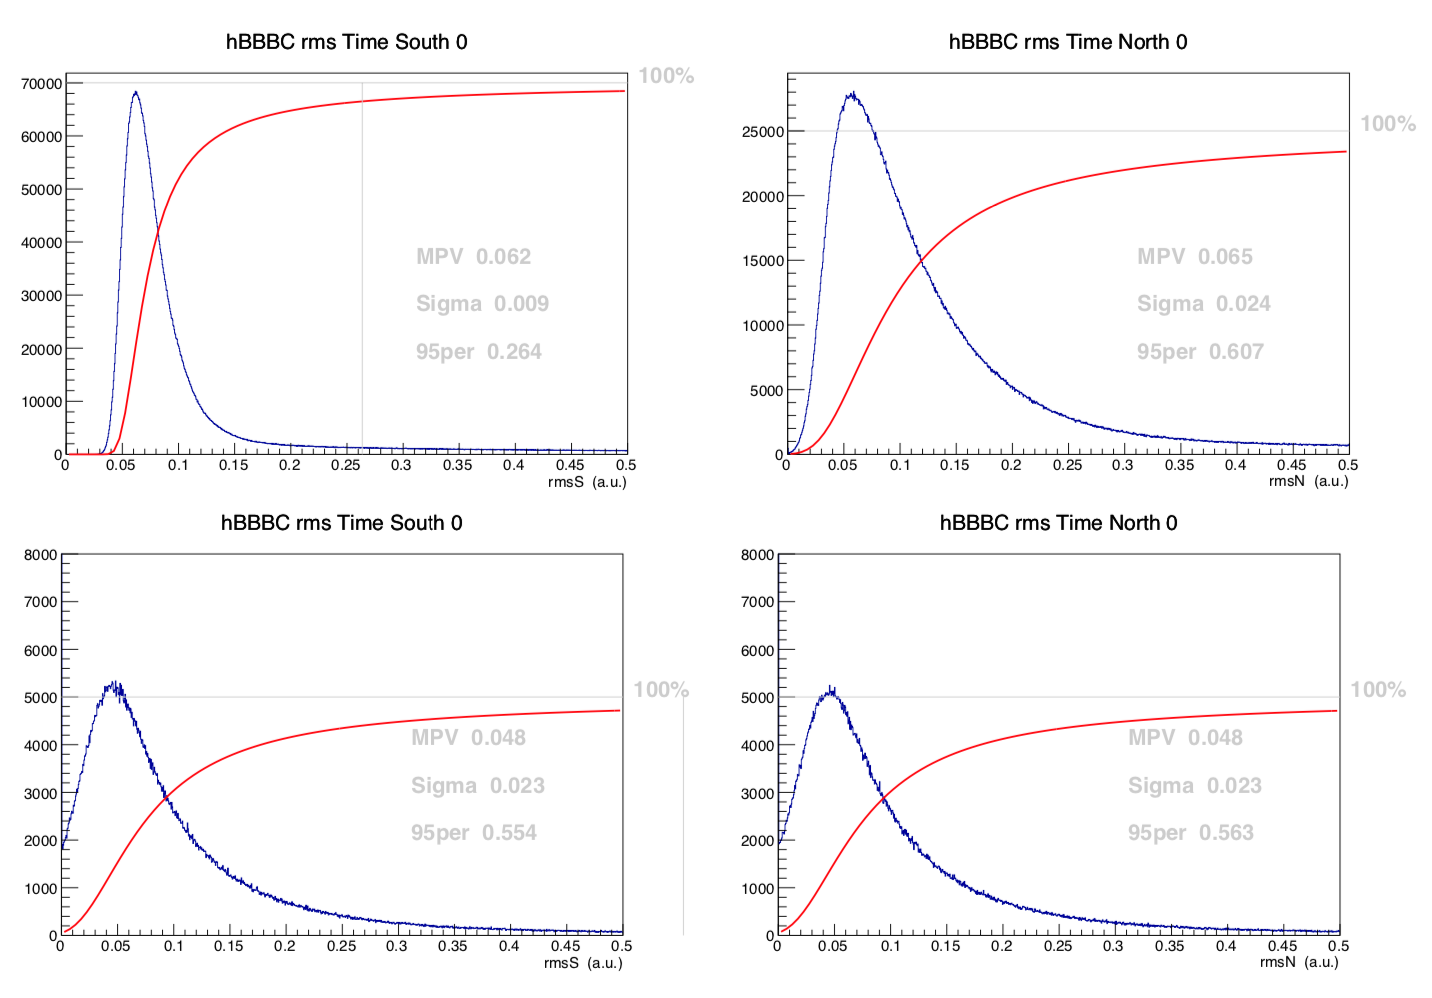
\includegraphics[width=\textwidth]{fig_pi0vn/bbc_timing_rms.png}
  \caption[BBC RMS Distribution]{BBC RMS Distribution, top pannels are 0-5$\%$ centrality and bottoms are inclusive, 
  red line is culmulative value}
  \label{fig:BBC Time RMS}
\end{figure}

\begin{figure}[!htb]
  \centering  
    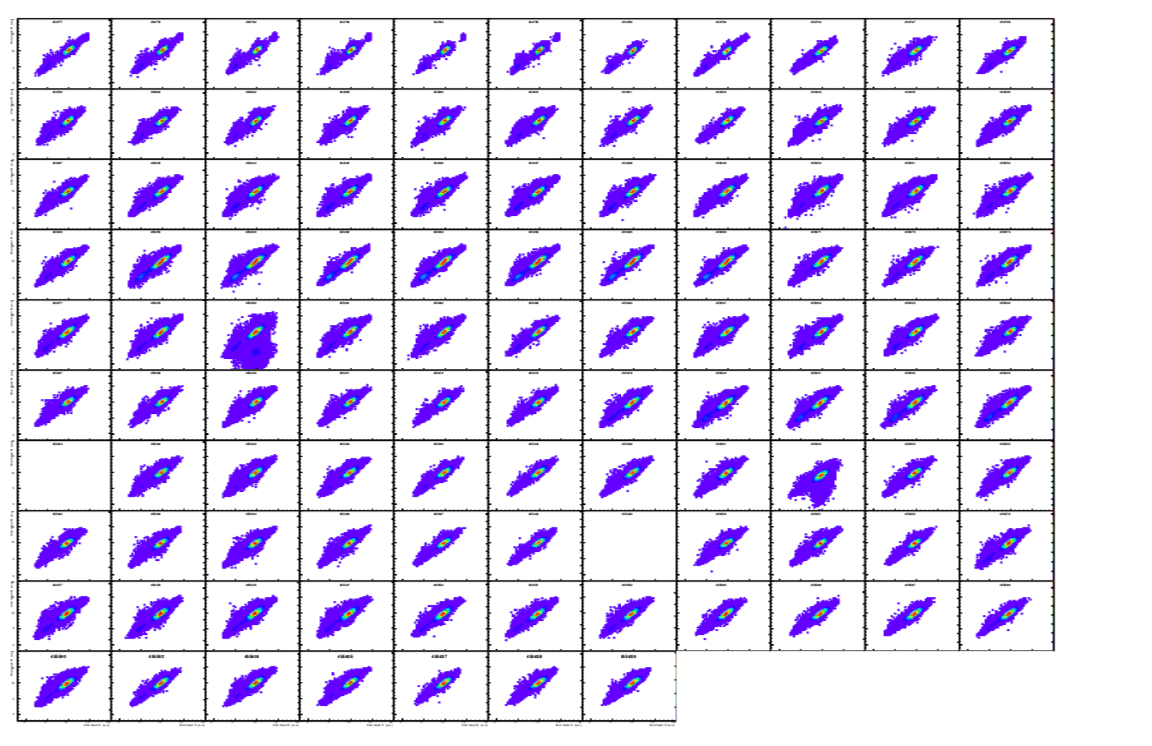
\includegraphics[width=\textwidth]{fig_pi0vn/bbc_timemean_corr.png}
  \caption[BBC Time Mean Coincident for Runs]{BBC Time Mean Coincident for Runs, Raw distribution of time coincidence for BBC (x-axis south, y-axis north) in dAu 
  collisions from 0 to 5$\%$ centrality at 200 GeV. Each pannel represents situation for one run.}
  \label{fig:BBC Time Mean Coincident for Runs}
\end{figure}

\begin{figure}[!htb]
  \centering  
    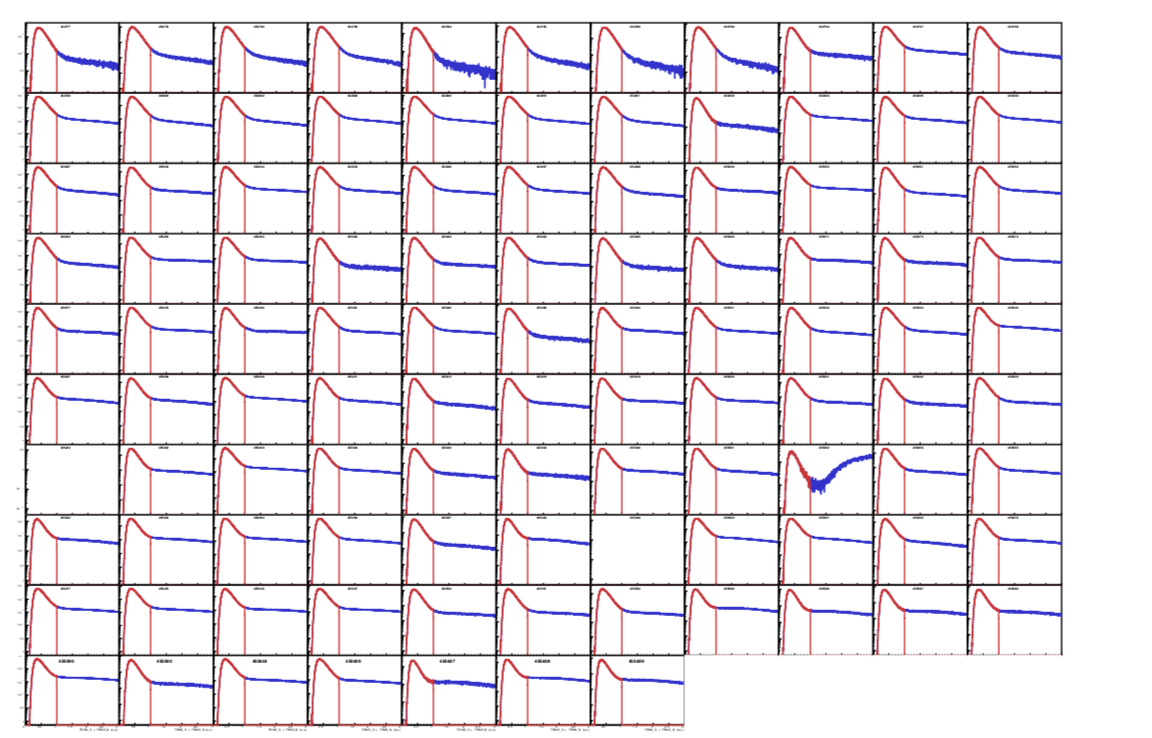
\includegraphics[width=\textwidth]{fig_pi0vn/bbc_timingrms_runs.png}
  \caption[BBC Time RMS for Runs]{BBC Time RMS for Runs, Raw distribution of BBC time RMS. red line indicating for cut for pileup rejection, Each pannel represents situation for one run.}
  \label{fig:BBC Time RMS for Runs}
\end{figure}

\begin{figure}[!htb]
  \centering  
    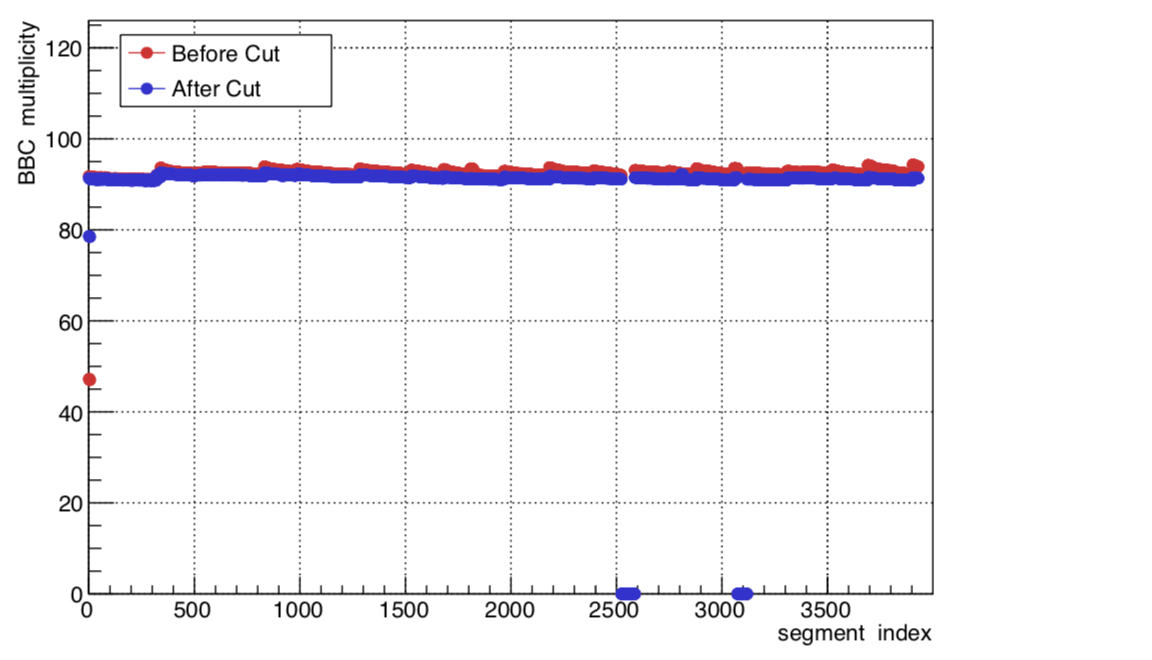
\includegraphics[width=\textwidth]{fig_pi0vn/bbc_activity_aftercut.png}
  \caption[BBC Activity After Cut]{BBC Activity After Cut, For each run (x-axis) fluctuation of BBC activity before and after cut}
  \label{fig:BBC Activity After Cut}
\end{figure}

\section{EMCal Calibration}

\subsection{ADC hit frequency}
The procedure for tagging bad towers followed here is based on the ones used for other analysis.
The tagging is done separately for the two triggers.

The hit frequency for every tower is analyzed statistically.
Towers with a hit frequency higher than 3 sigma were rejected.

\begin{figure}
  \centering
  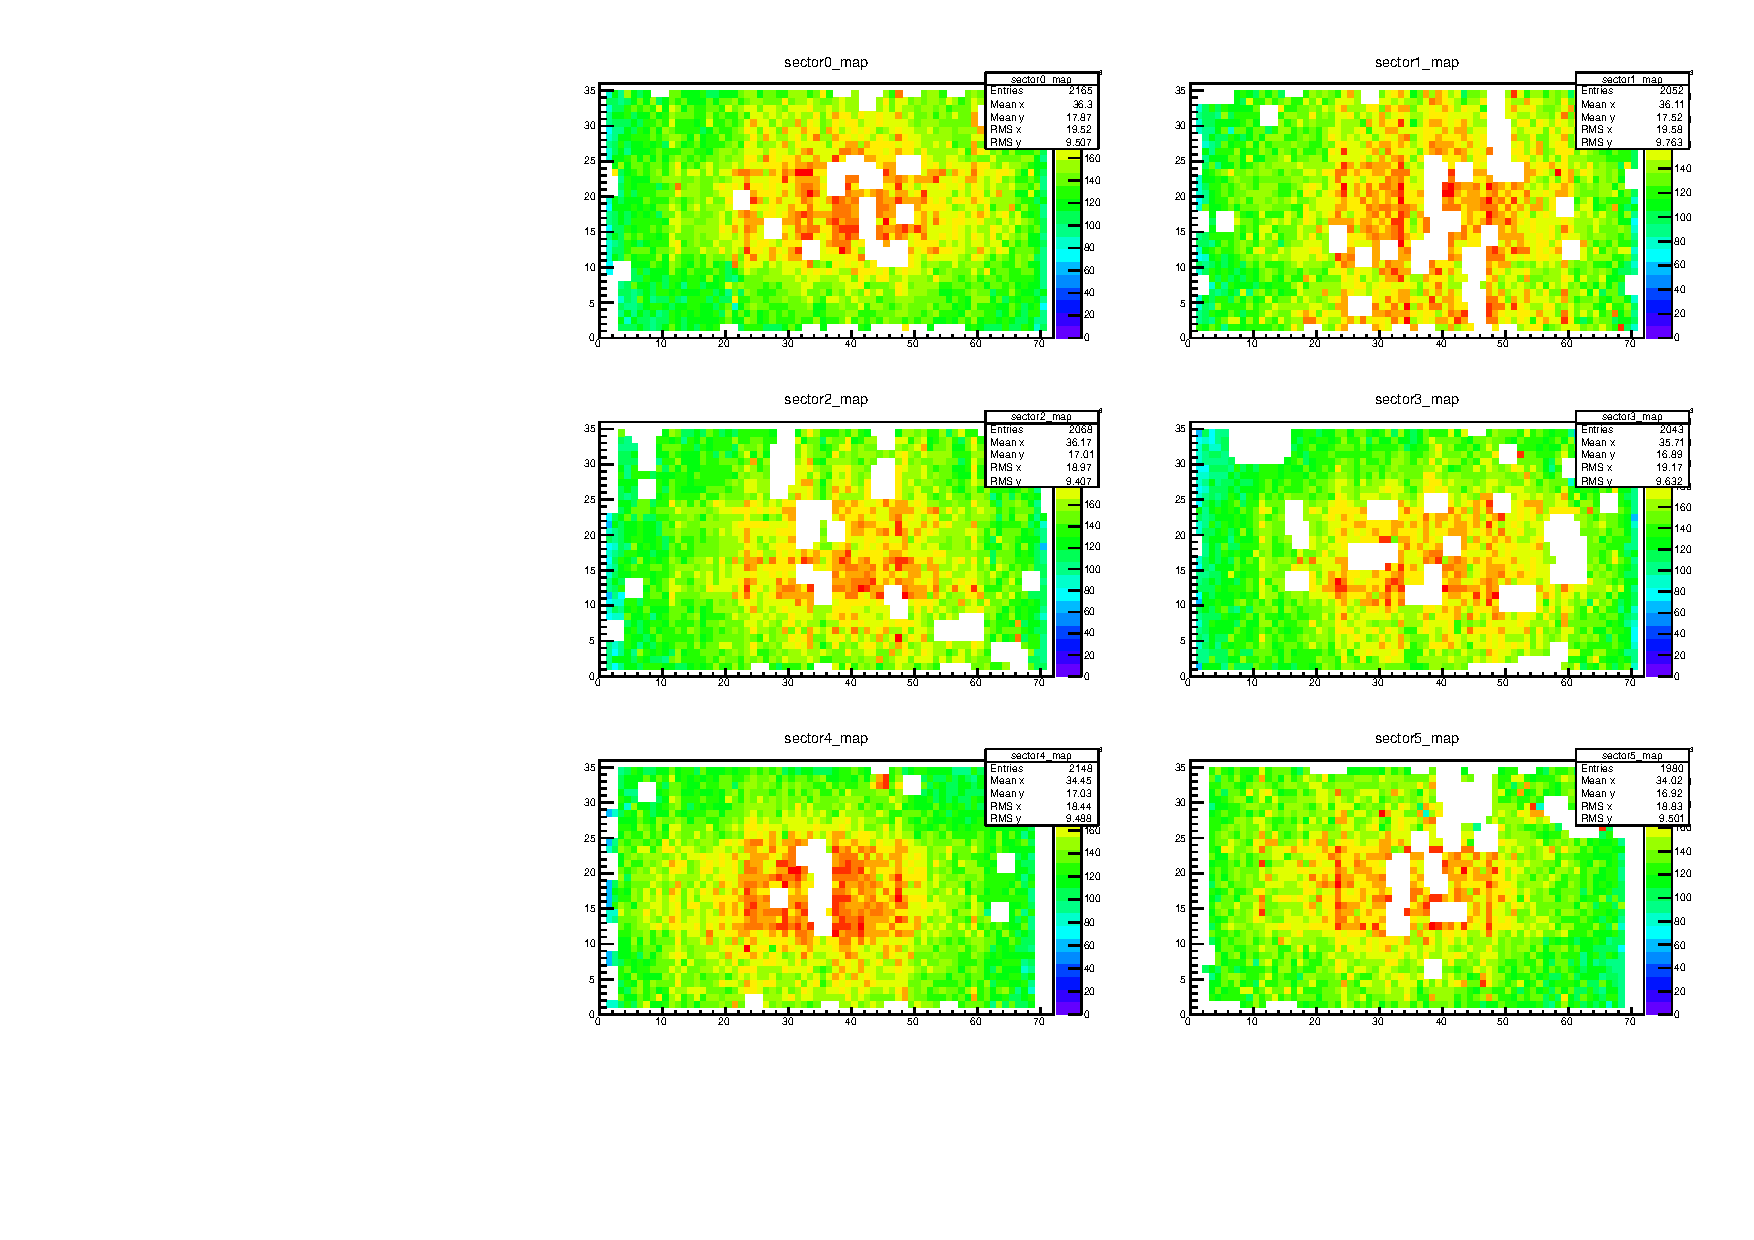
\includegraphics[width=1\textwidth]{fig_pi0vn/sect_0-5_masked.pdf} \\
  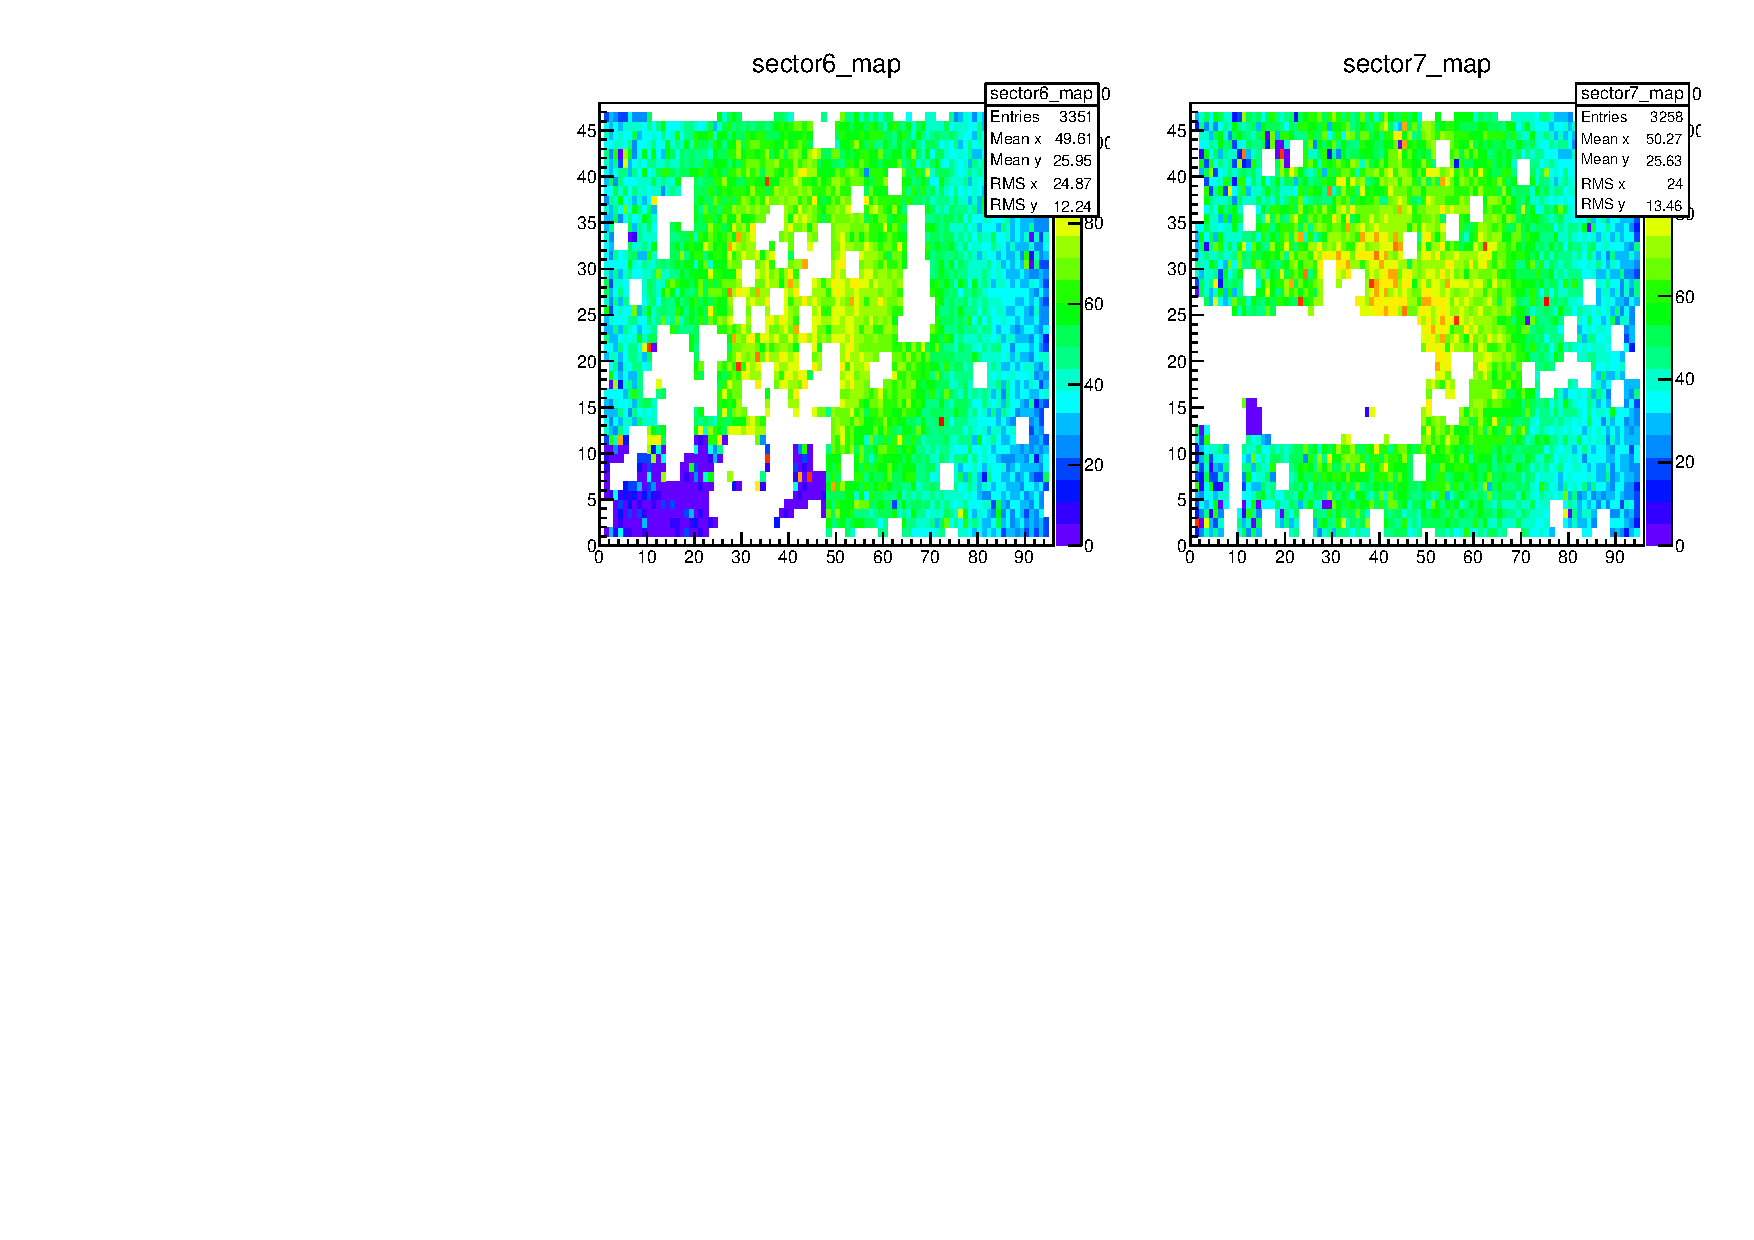
\includegraphics[width=1\textwidth]{fig_pi0vn/sect_6-7_masked.pdf} 
  \caption{Hit frequency per tower in d+Au at 200 GeV for the PbSc (top six plots) and PbGl (bottom plots) after removing outliers beyond three sigma.}
  \label{sect05masked}
\end{figure}
\begin{figure}
  \centering
  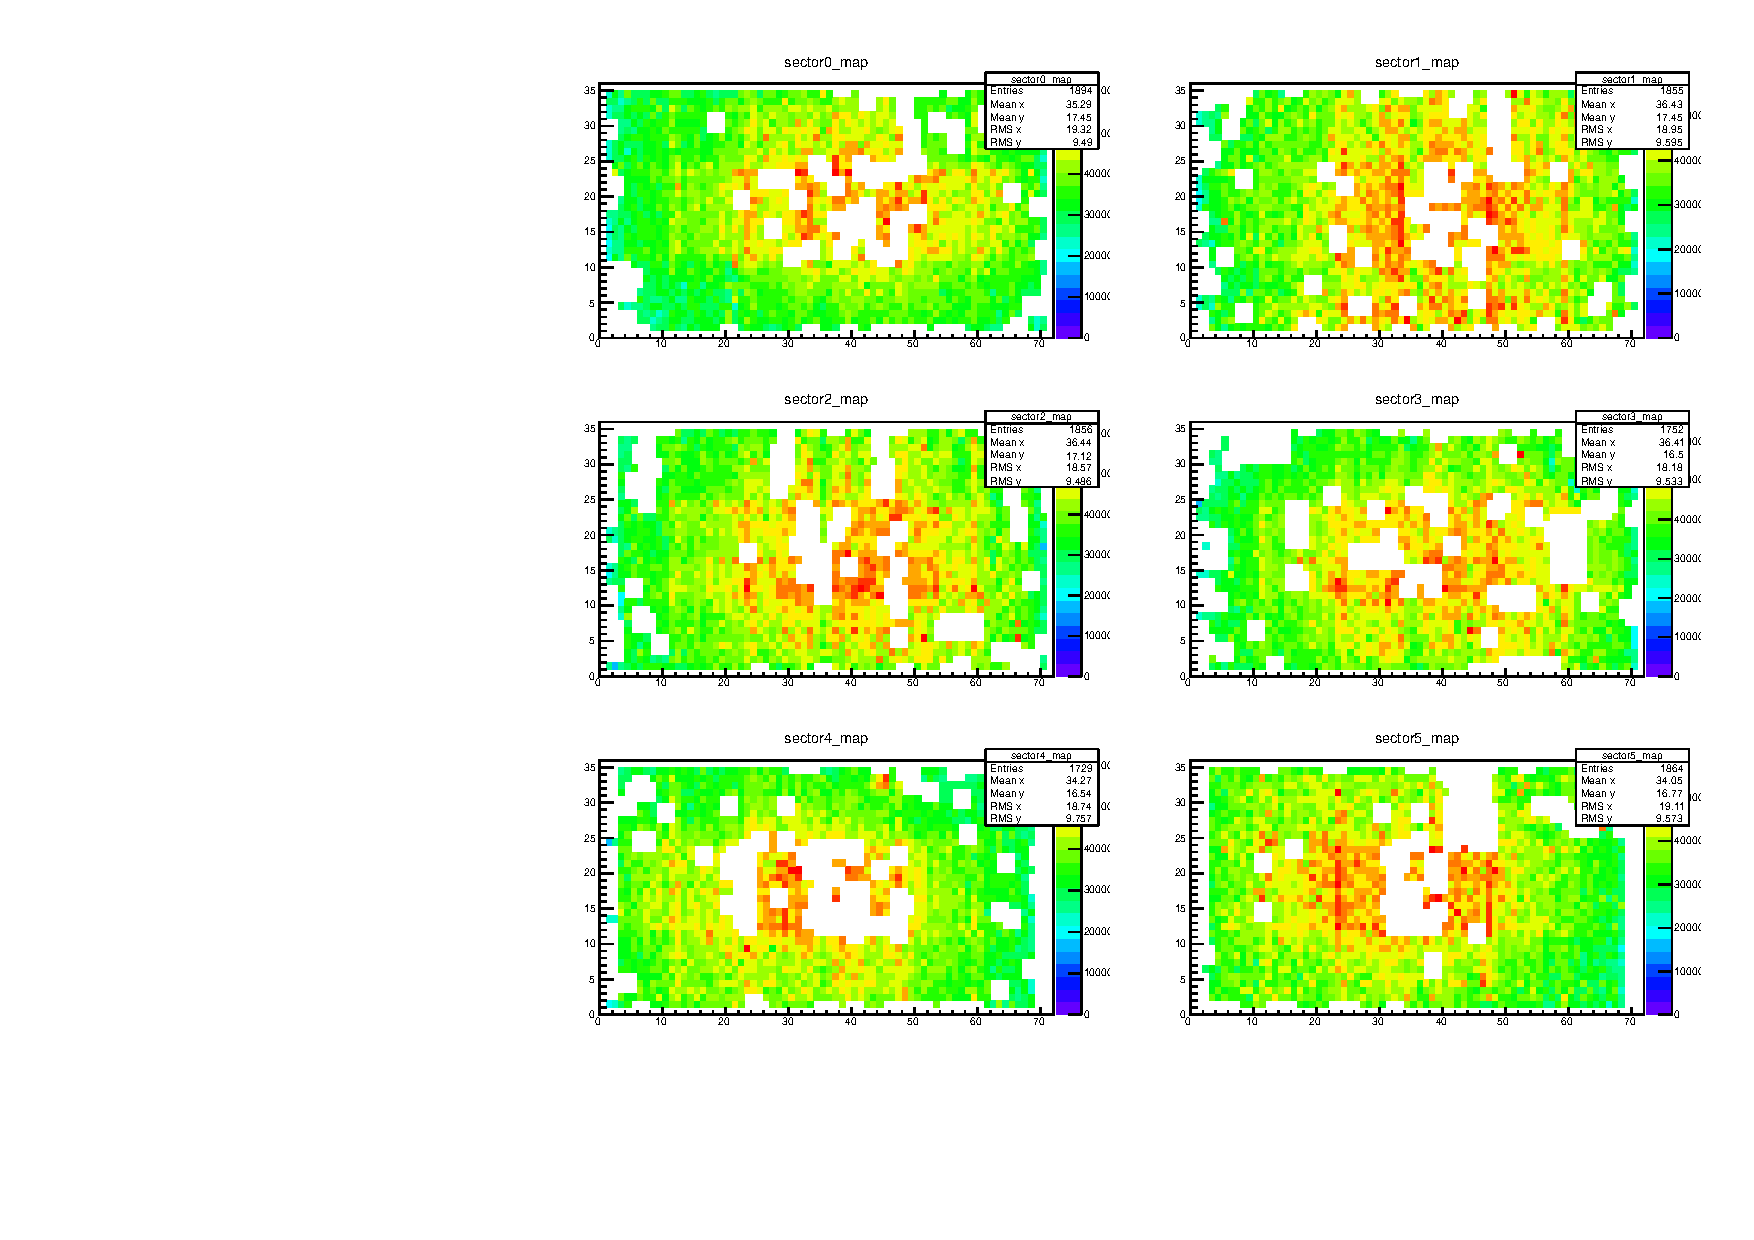
\includegraphics[width=1\textwidth]{fig_pi0vn/deadmap_sect0-5_62GEV.pdf}
  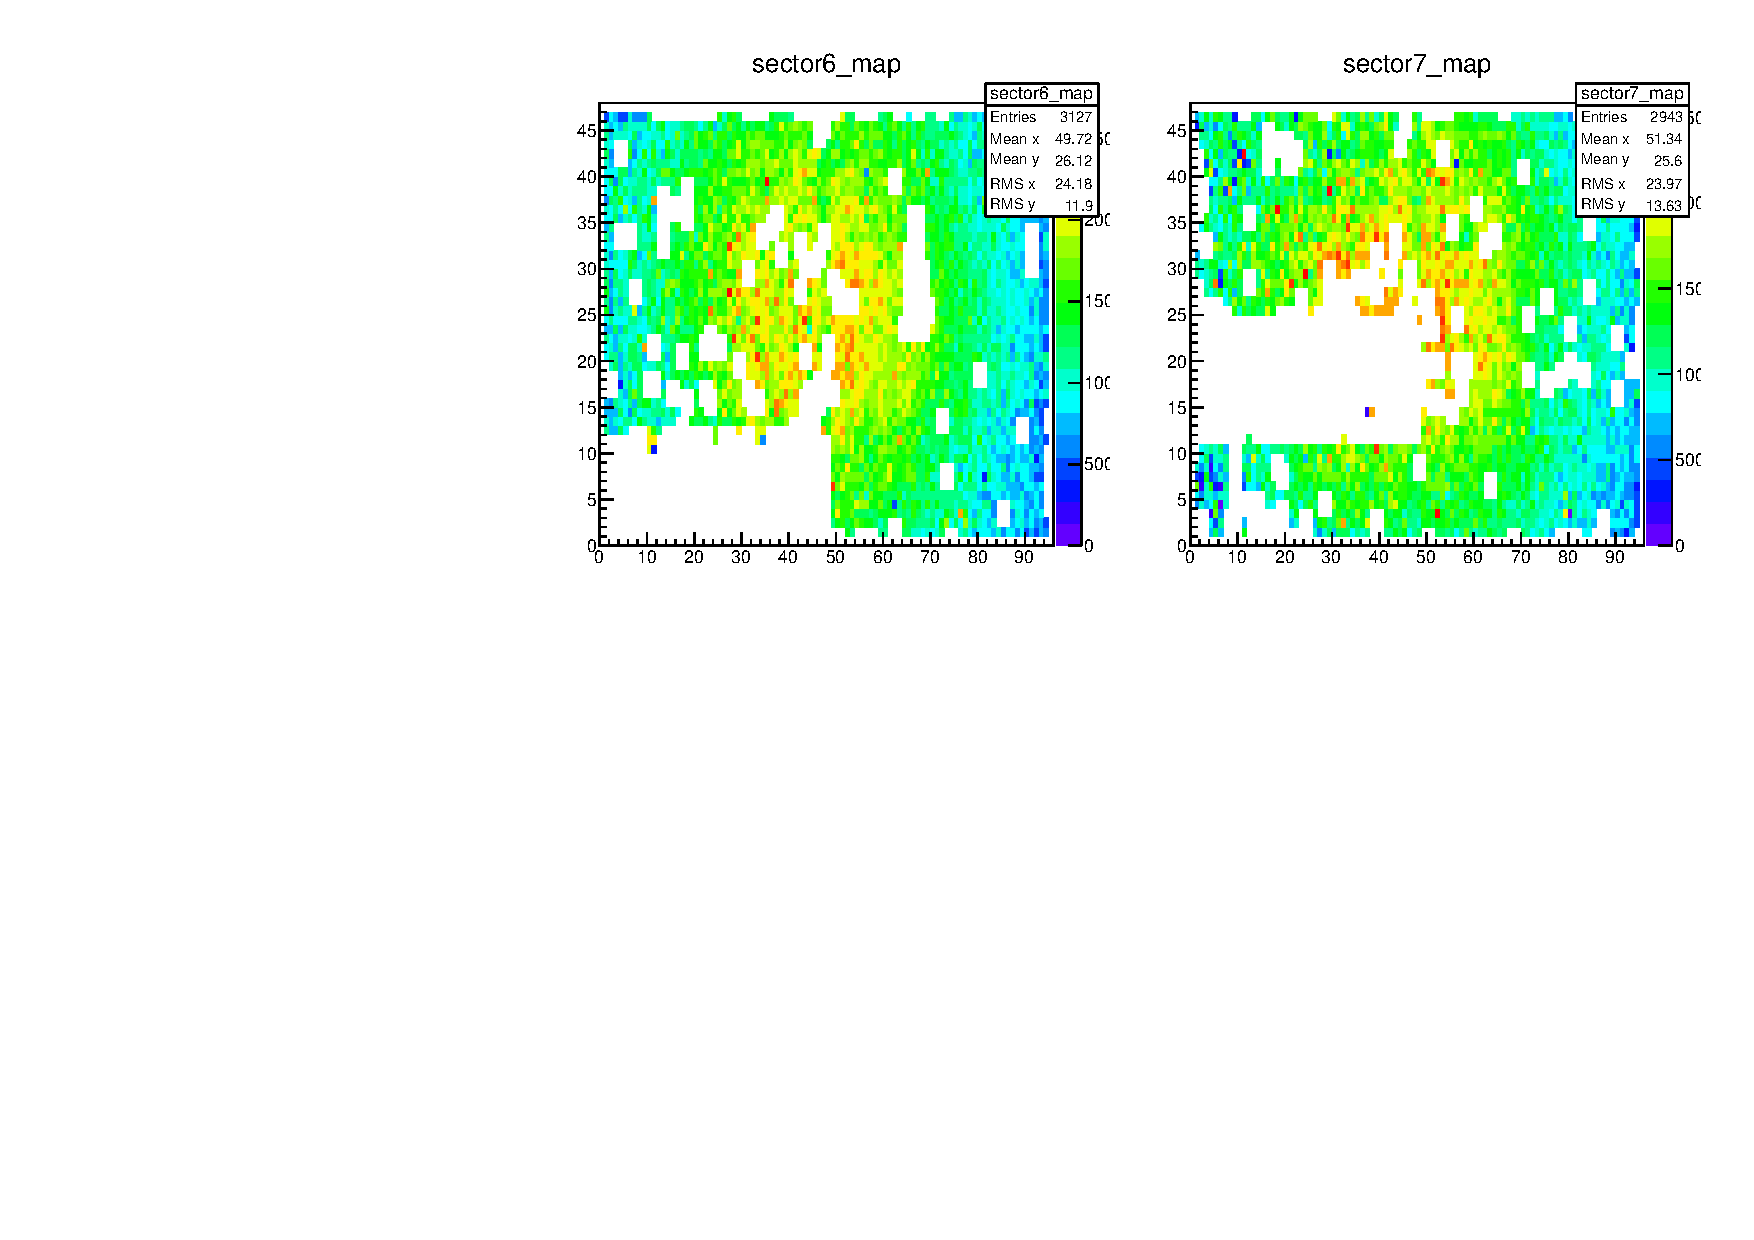
\includegraphics[width=1\textwidth]{fig_pi0vn/deadmap_sect6-7_62GEV.pdf}
  \caption{Hit frequency per tower in d+Au at 62 GeV for the PbSc (top six plots) and PbGl (bottom plots) after removing outliers beyond three sigma.}
  \label{sectmasked.62GeV}
\end{figure}
After the bad towers are identified, the 3x3 region surrounding the problematic tower is also removed.
In addition, the towers on the border of each section is tagged as well.
For MB triggered data, each sector is analyzed in four energy bins: [0.2-0.5] GeV, [0.5-1] GeV, [1-2] GeV and [2-4] GeV and for the ERT triggered data [0.5-2], [2-10]GeV.
\newline
The percentage of towers unusable as cluster centers is shown in tables \ref{table:table warnmap}.
\begin{table}[htb!]
  \begin{center}
    \begin{tabular}{||c|c|c|c|c||} 
\hline Sector & Tagged(MB) & Masked(MB) & Tagged(ERT) & Masked(ERT) \\ \hline
0 & 8.6 & 17 & 9.3 & 16.8 \\ \hline
1 & 14 & 22.2 & 14.3 & 22.1 \\ \hline
2 & 12.3 & 20.6 & 13 & 20 \\ \hline
3 & 13.3 & 21.7 & 13.9 & 21.5 \\ \hline
4 & 14.9 & 23.2 & 15.4 & 23 \\ \hline
5 & 16.7 & 25 & 17.6 & 24.8 \\ \hline
6 & 22.8 & 29 & 23.6 & 28.9 \\ \hline
7 & 28.3 & 34.6 & 28.8 & 34.5 \\ \hline
    \end{tabular}
  \end{center}
  \caption[Percentage of towers unusable as cluster center for d+Au at 200 GeV per sector]{Percentage of towers unusable as cluster center for d+Au at 200 GeV per sector. "Tagged" corresponds to those tagged 
  based on ADC hit frequency and its 3x3 neighbors; "Masked" including "Tagged" and towers at borders.}
  \label{table:table warnmap}
\end{table}
\subsection{Energy correction}
The procedure for energy calibration used here is based on that performed in other analysis, CITE OTHER ANALYSIS NOTES. 
The EMCal energy calibration sector by sector is done here with the MB dataset.
It is needed to set an overall energy scale and equalize the $\pi^{0}$ mass peak over all sectors and for each run.

For this part, $\pi^{0}$ candles reconstructed using nominal cuts (see next section) with transverse momentum in the range from 3-10 GeV/c was used as done in previous analysis.
From the $\pi^{0}$ invariant mass distribution the position of the resonance mass is extracted as a function of the run number for each sector.
The energy per sector was corrected so that the resonance mass sits at 138 MeV in order to match the output of the embedded simulation as reported in CITE NOTE.
The result for the recalibration of 200 GeV is shown in figure \ref{recalib200GeV} for each sector before and after the recalibration.
This recalibration is done by a local recalibrator.
\begin{figure}
    \centering
    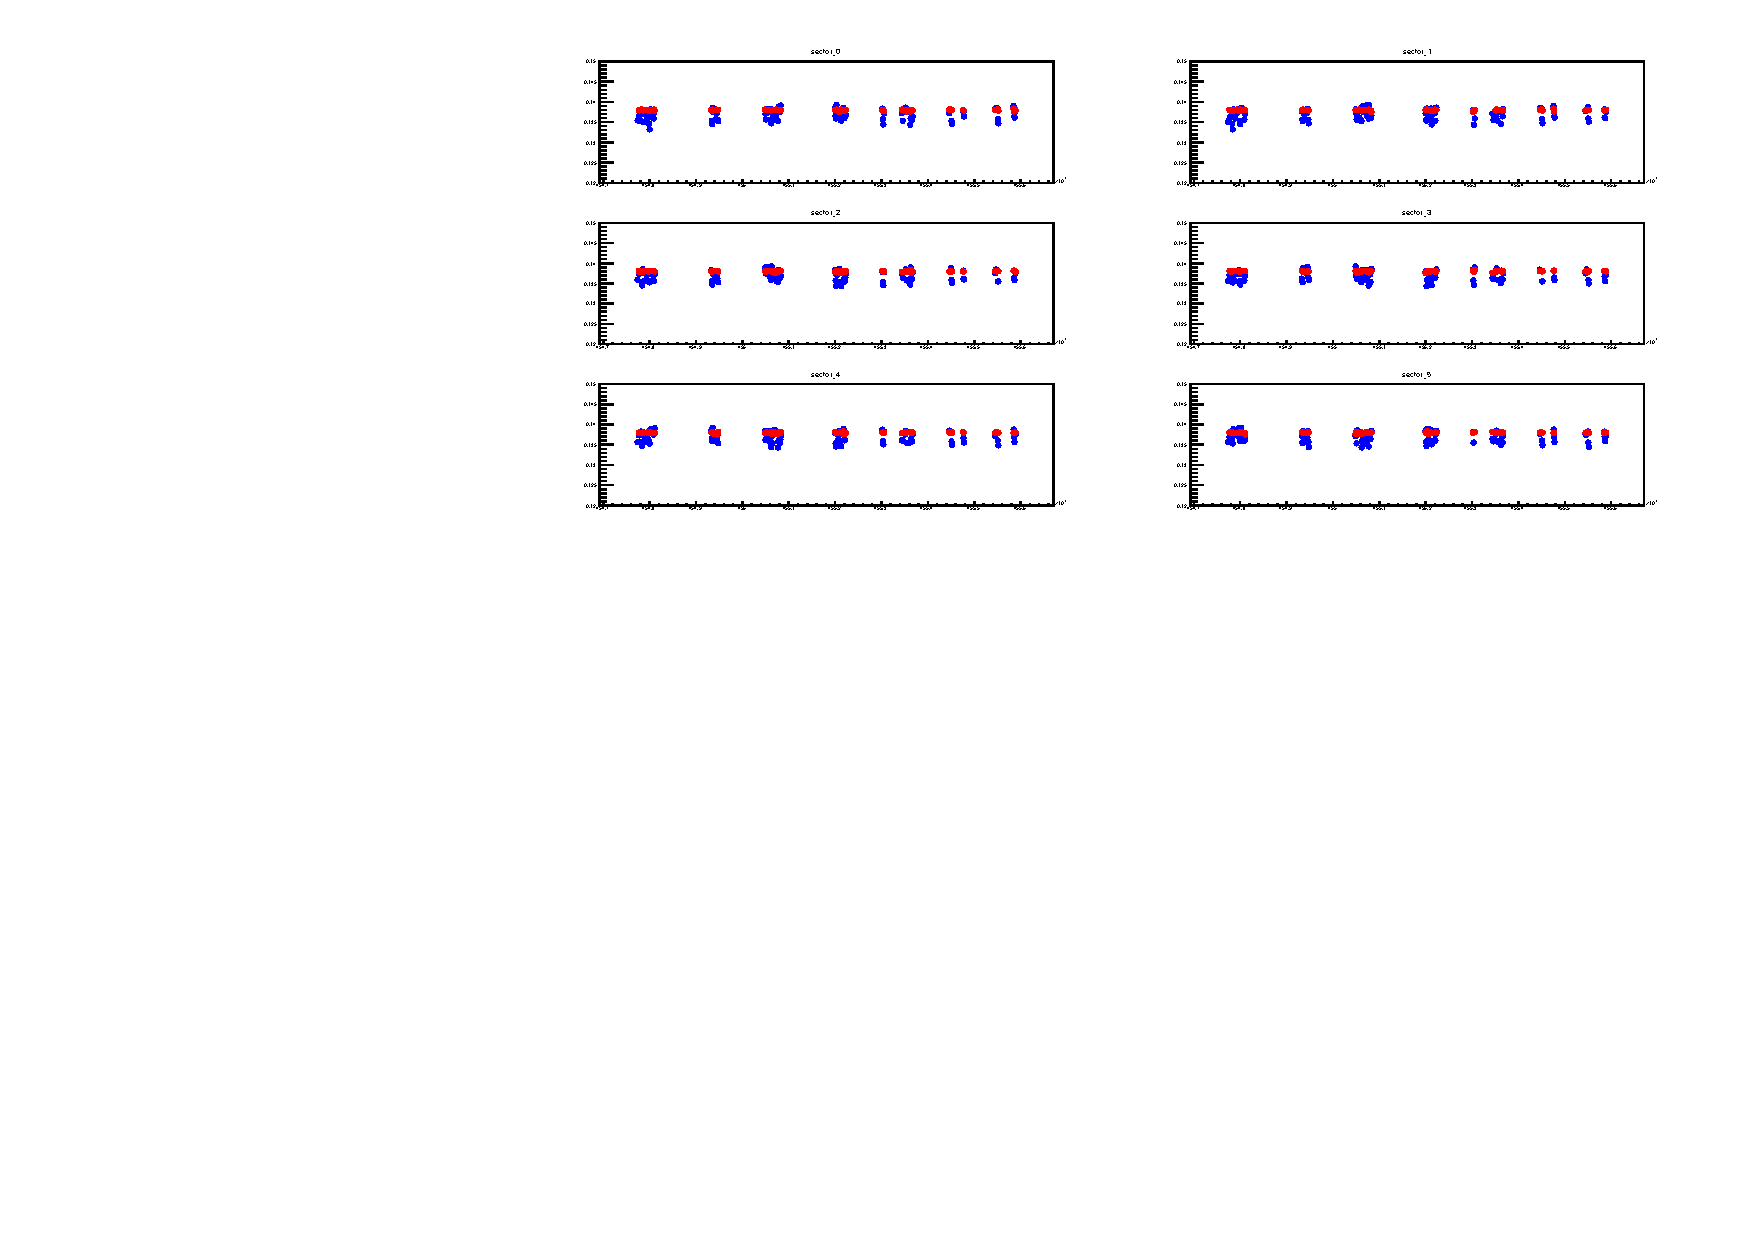
\includegraphics[width=1\textwidth]{fig_pi0vn/mean_pi0vsrun_sect0-5}
    \caption{dAu 200 GeV, Energy recalibration of PbSc sector . Mean $\pi^{0}$ peak before(blue) and after(red) calibration for all the runs}
    \label{recalib200GeV}
\end{figure}
\begin{figure}
    \centering
    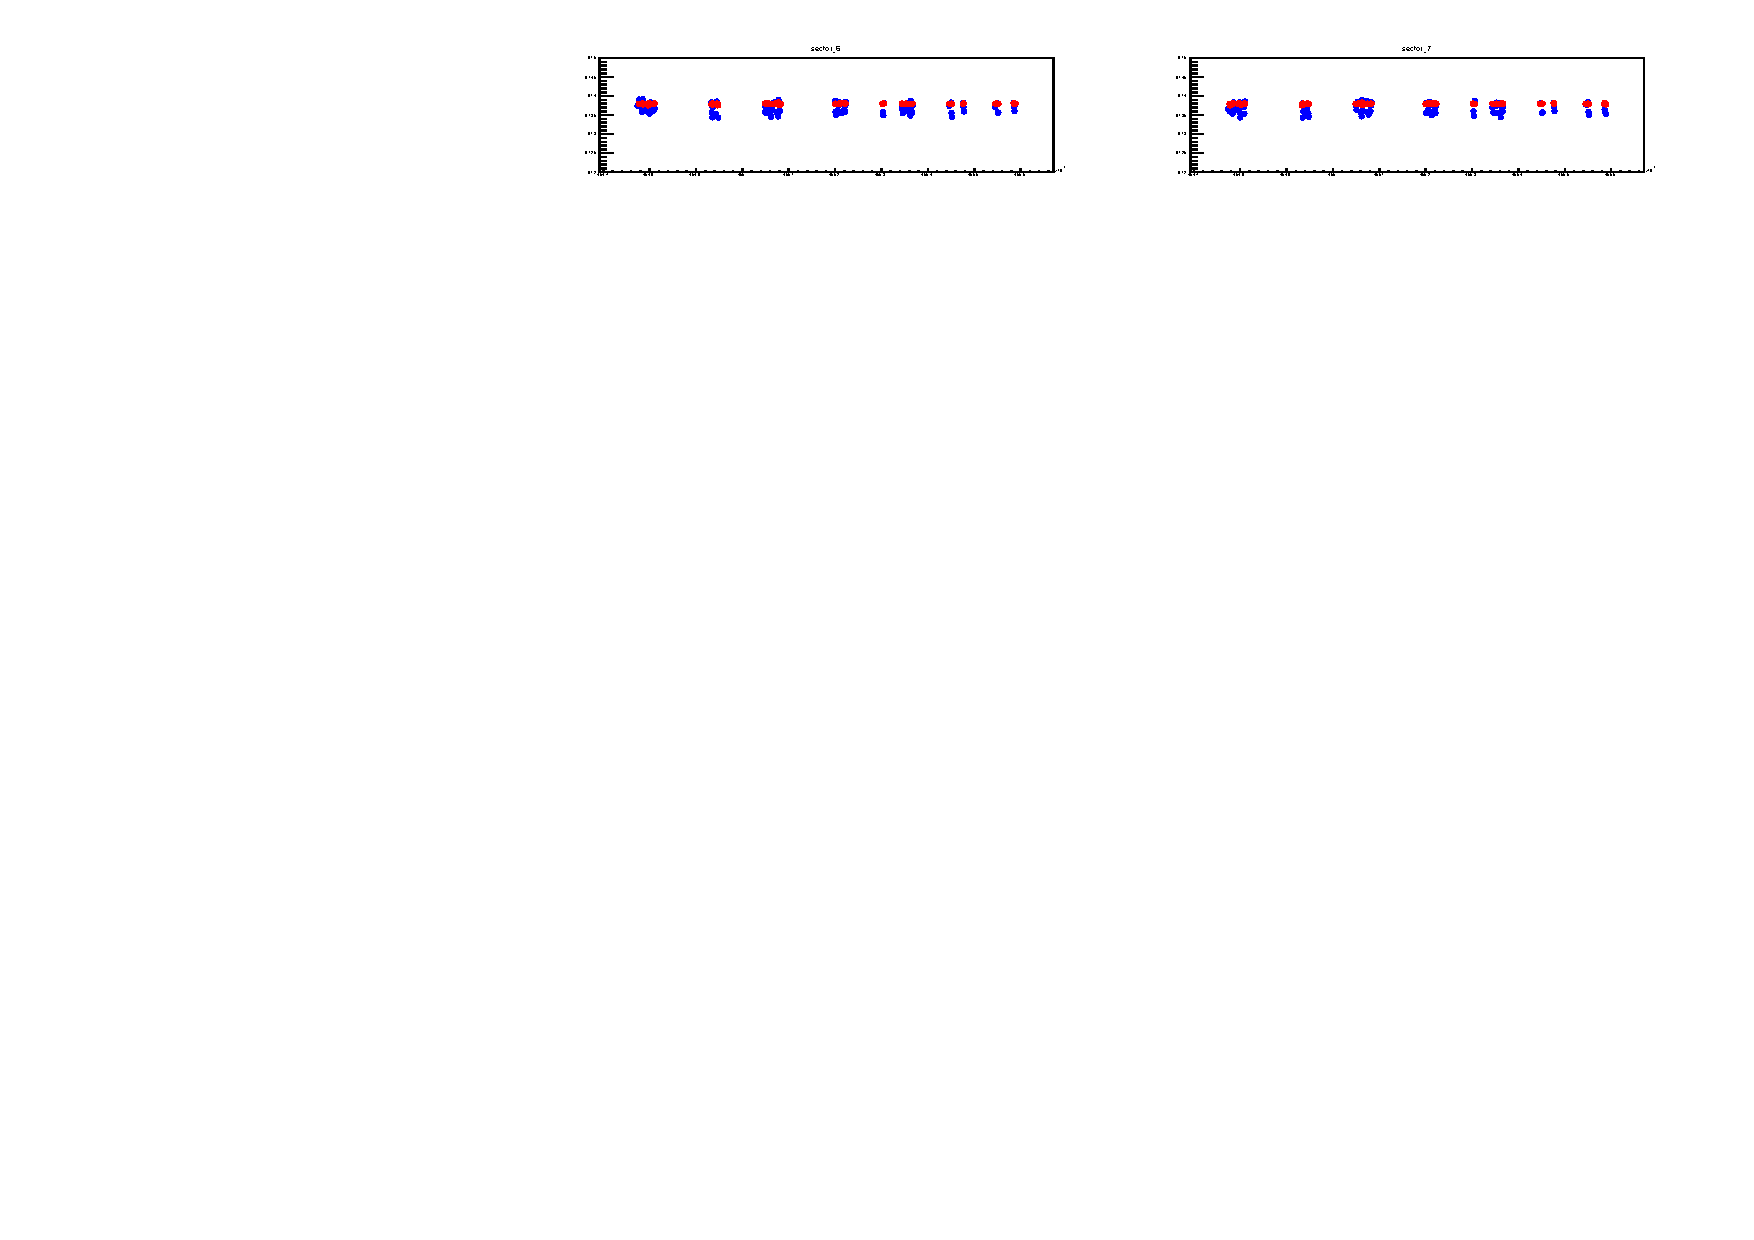
\includegraphics[width=1\textwidth]{fig_pi0vn/mean_pi0vsrun_sect6-7}
    \caption{dAu 200 GeV, Energy recalibration of PbGl sector. Mean $\pi^{0}$ peak before(blue) and after(red) calibration for all the runs}
    \label{meanpi0vsrunsect67}
\end{figure}
The figure \ref{sigma200GeV} shows the sigma of the $\pi^{0}$ peak vs pT for sector 1 and sector 6. 
\begin{figure}
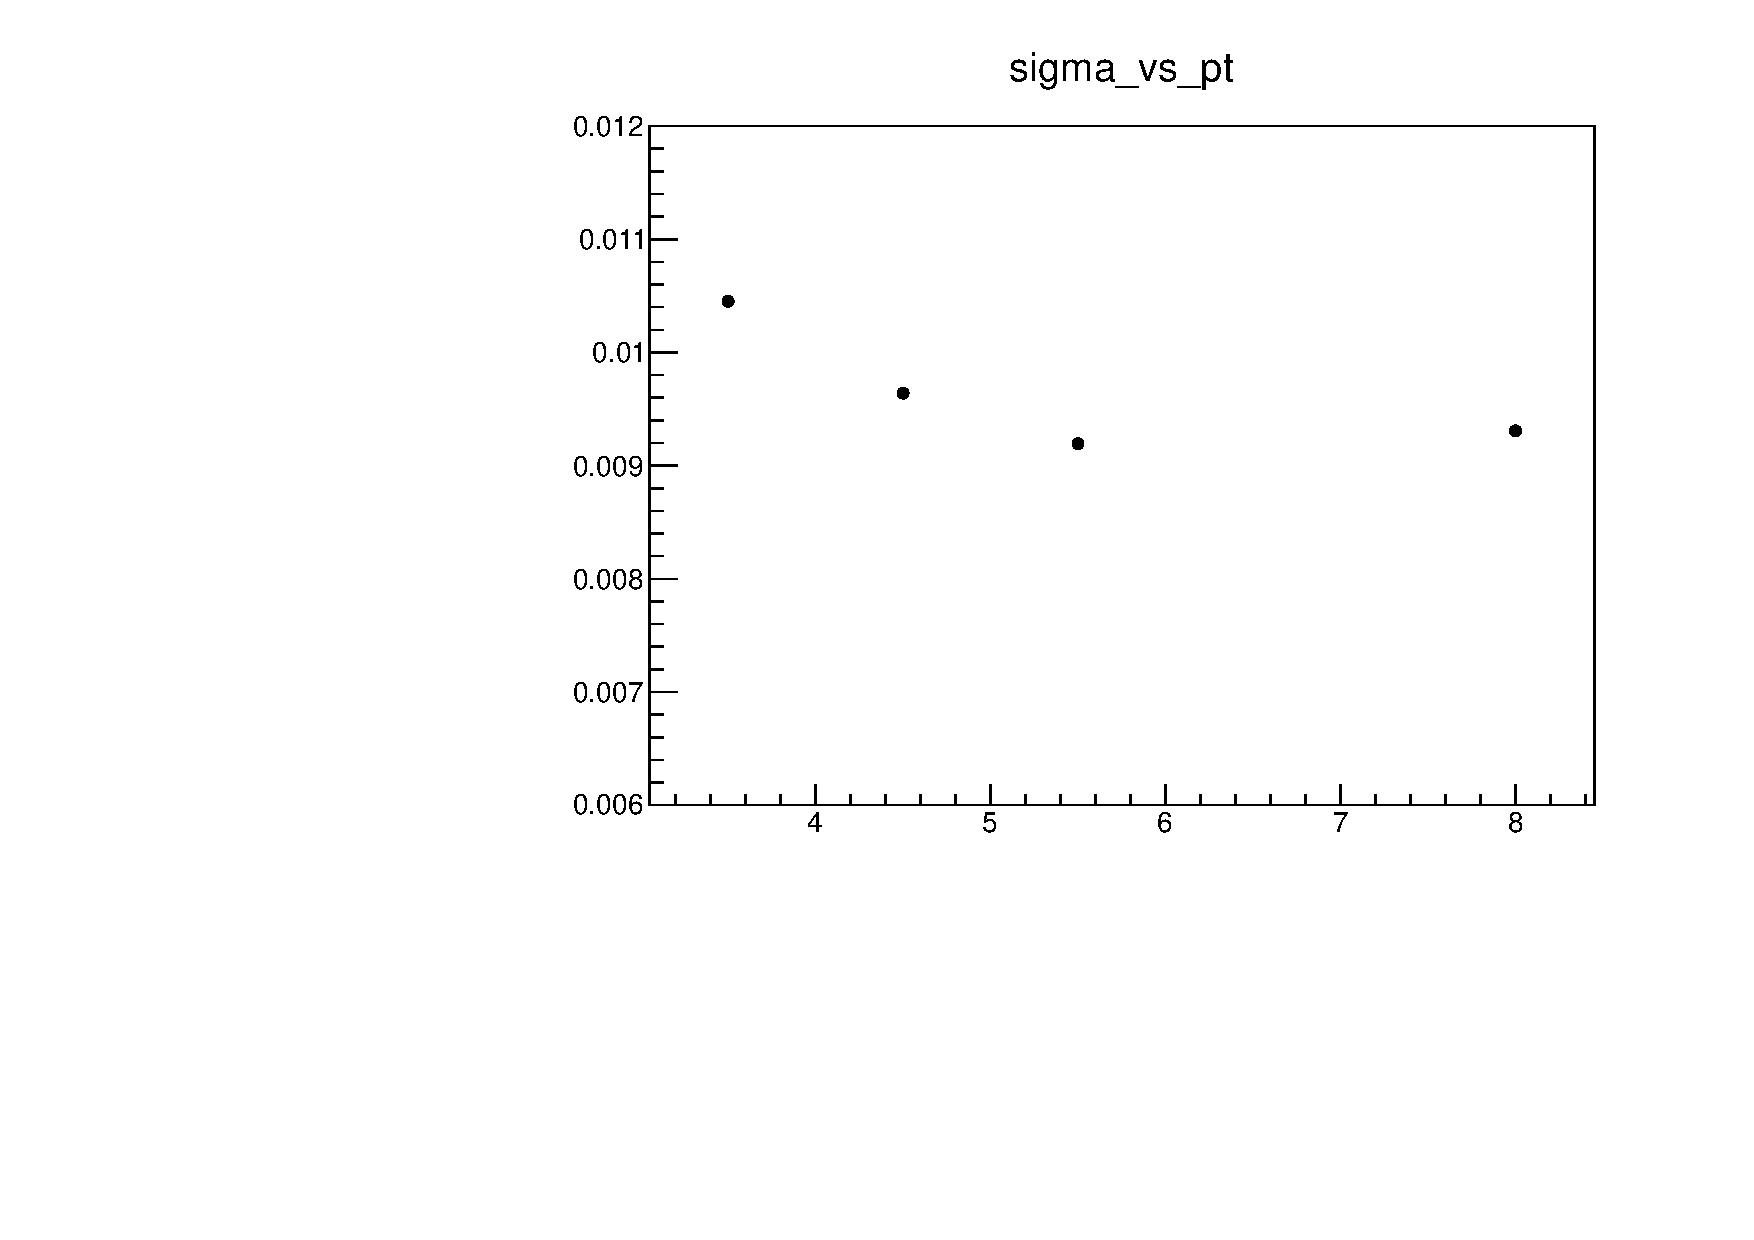
\includegraphics[width=0.47\textwidth]{fig_pi0vn/sect1_sigmavspt.pdf}
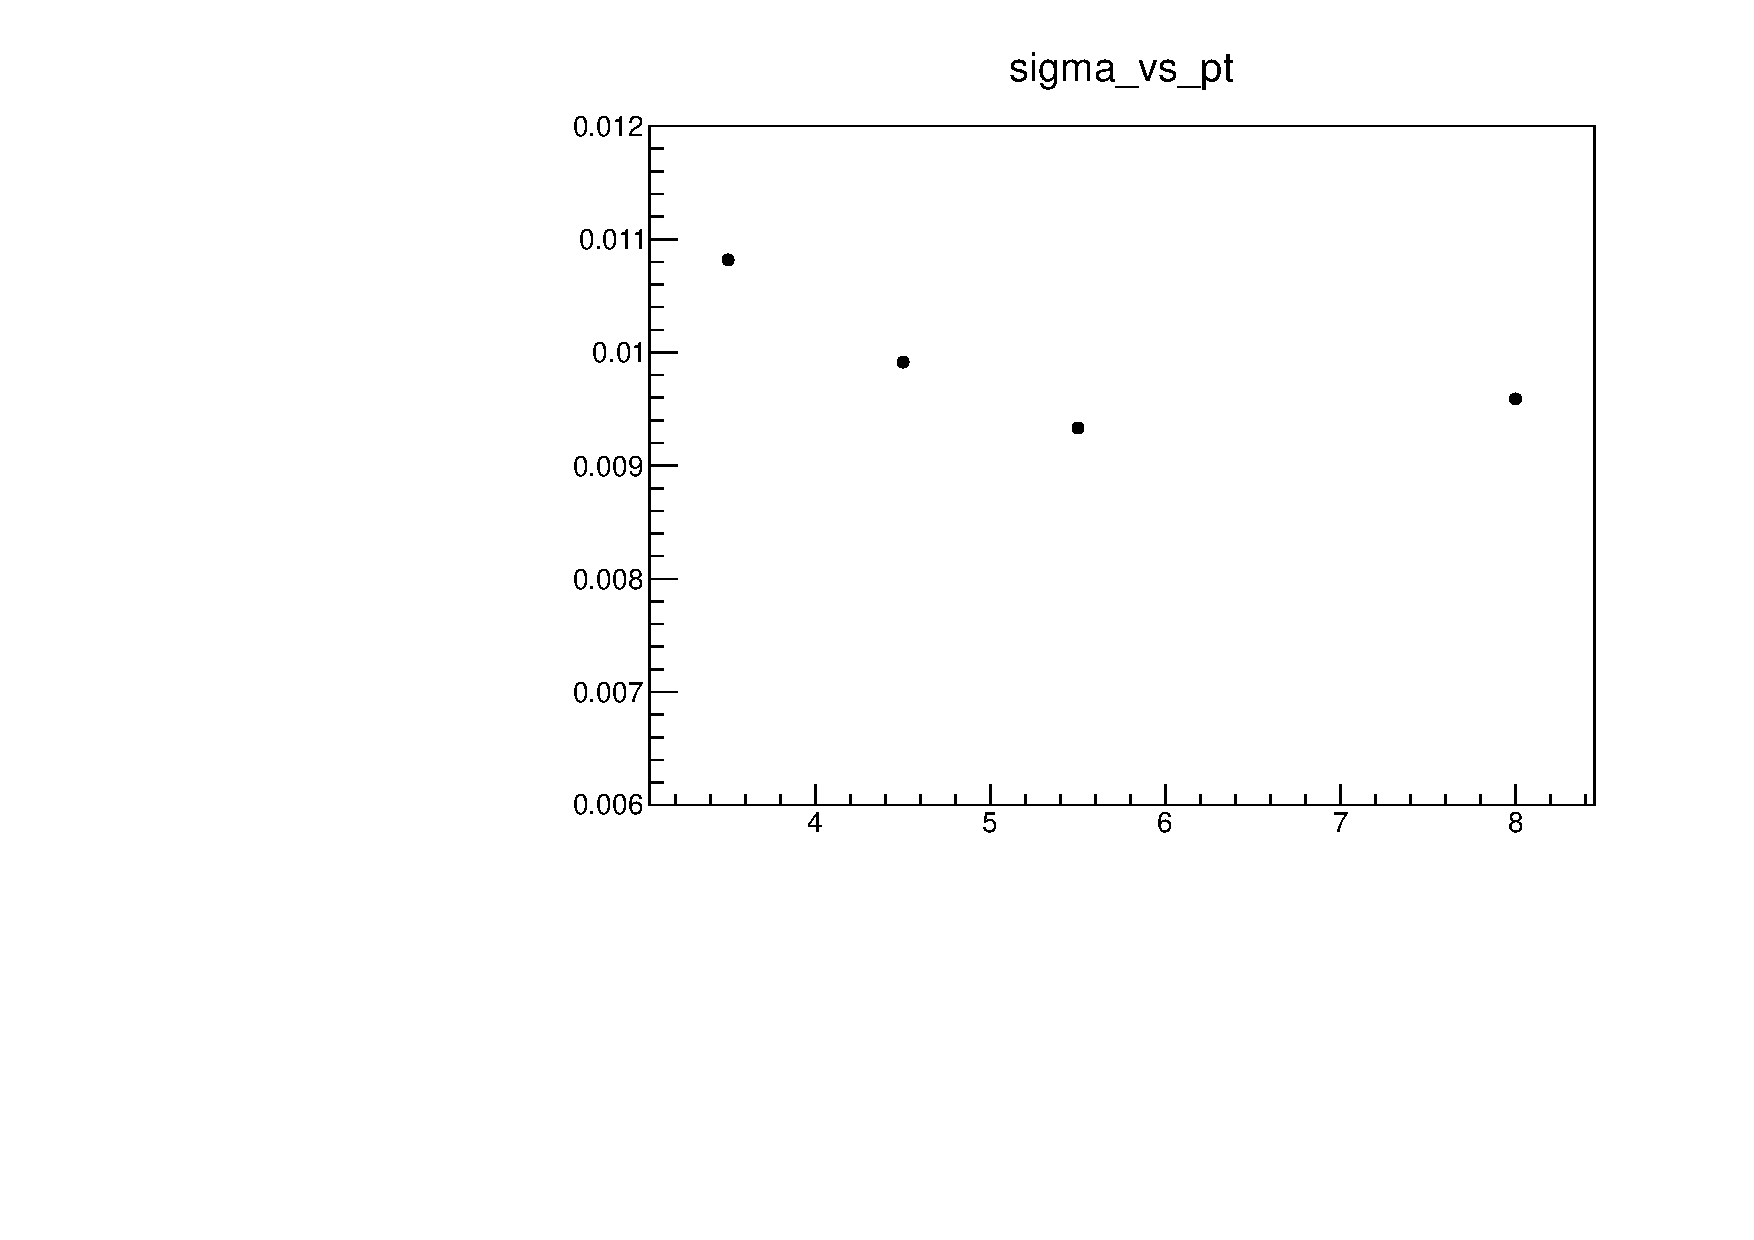
\includegraphics[width=0.47\textwidth]{fig_pi0vn/sect6_sigmavspt.pdf}
\caption{Sigma of the $\pi^{0}$ peak vs $p_{T}$ for sector 1 (left) and sector 6 (right). $3<p_{T}<10GeV$ ,200 GeV}
\label{sigma200GeV}
\end{figure}
\subsubsection{62 GeV}
The result for the recalibration of 62 GeV is shown in figure \ref{recalib62GeV} for each sector before and after the recalibrations for each run.
\begin{figure}
    \centering
    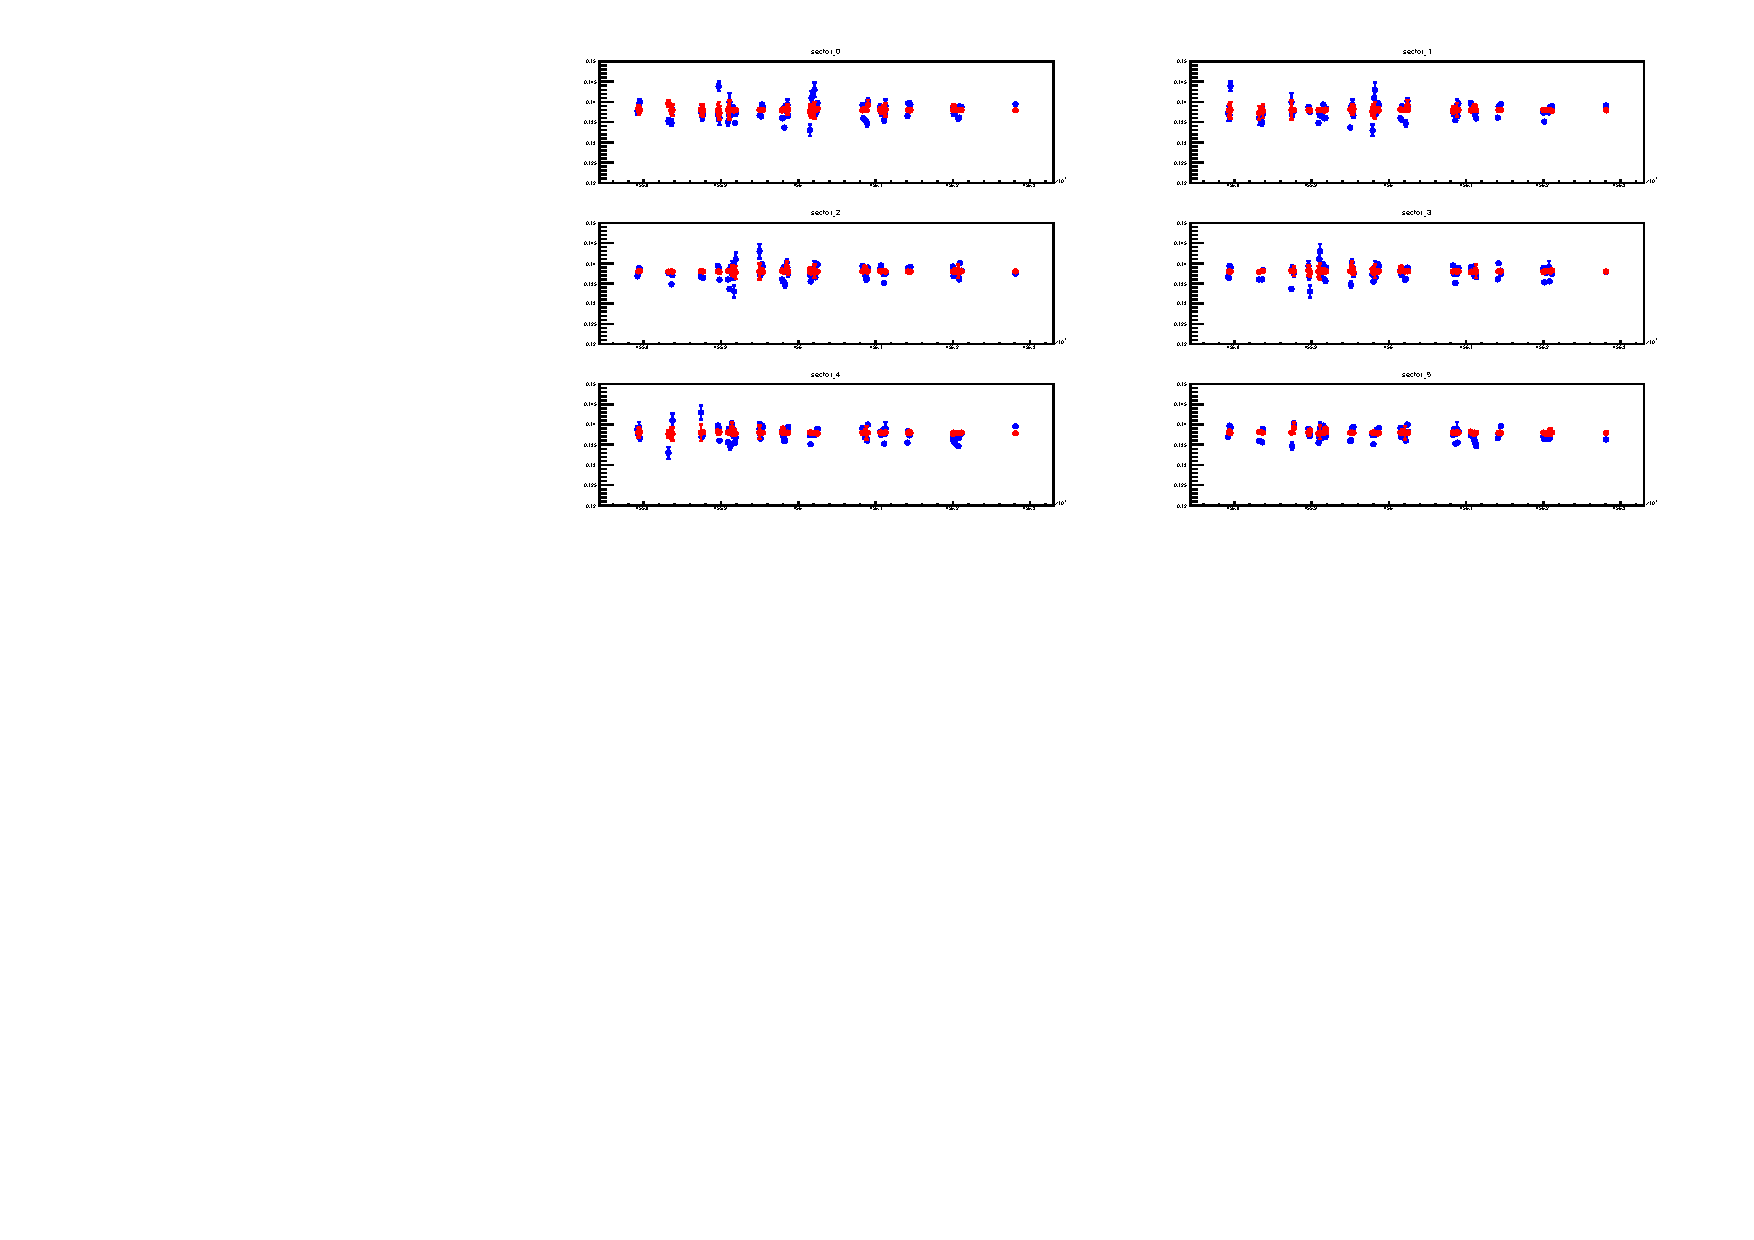
\includegraphics[width=1\textwidth]{fig_pi0vn/nocalib_vs_calib_sector1_6.pdf}
    \caption{dAu 62 GeV, Energy recalibration of PbSc sectors, Mean $\pi^{0}$ peak before(blue) and after(red) calibration for all the runs}
    \label{recalib62GeV}
\end{figure}
\begin{figure}
    \centering
    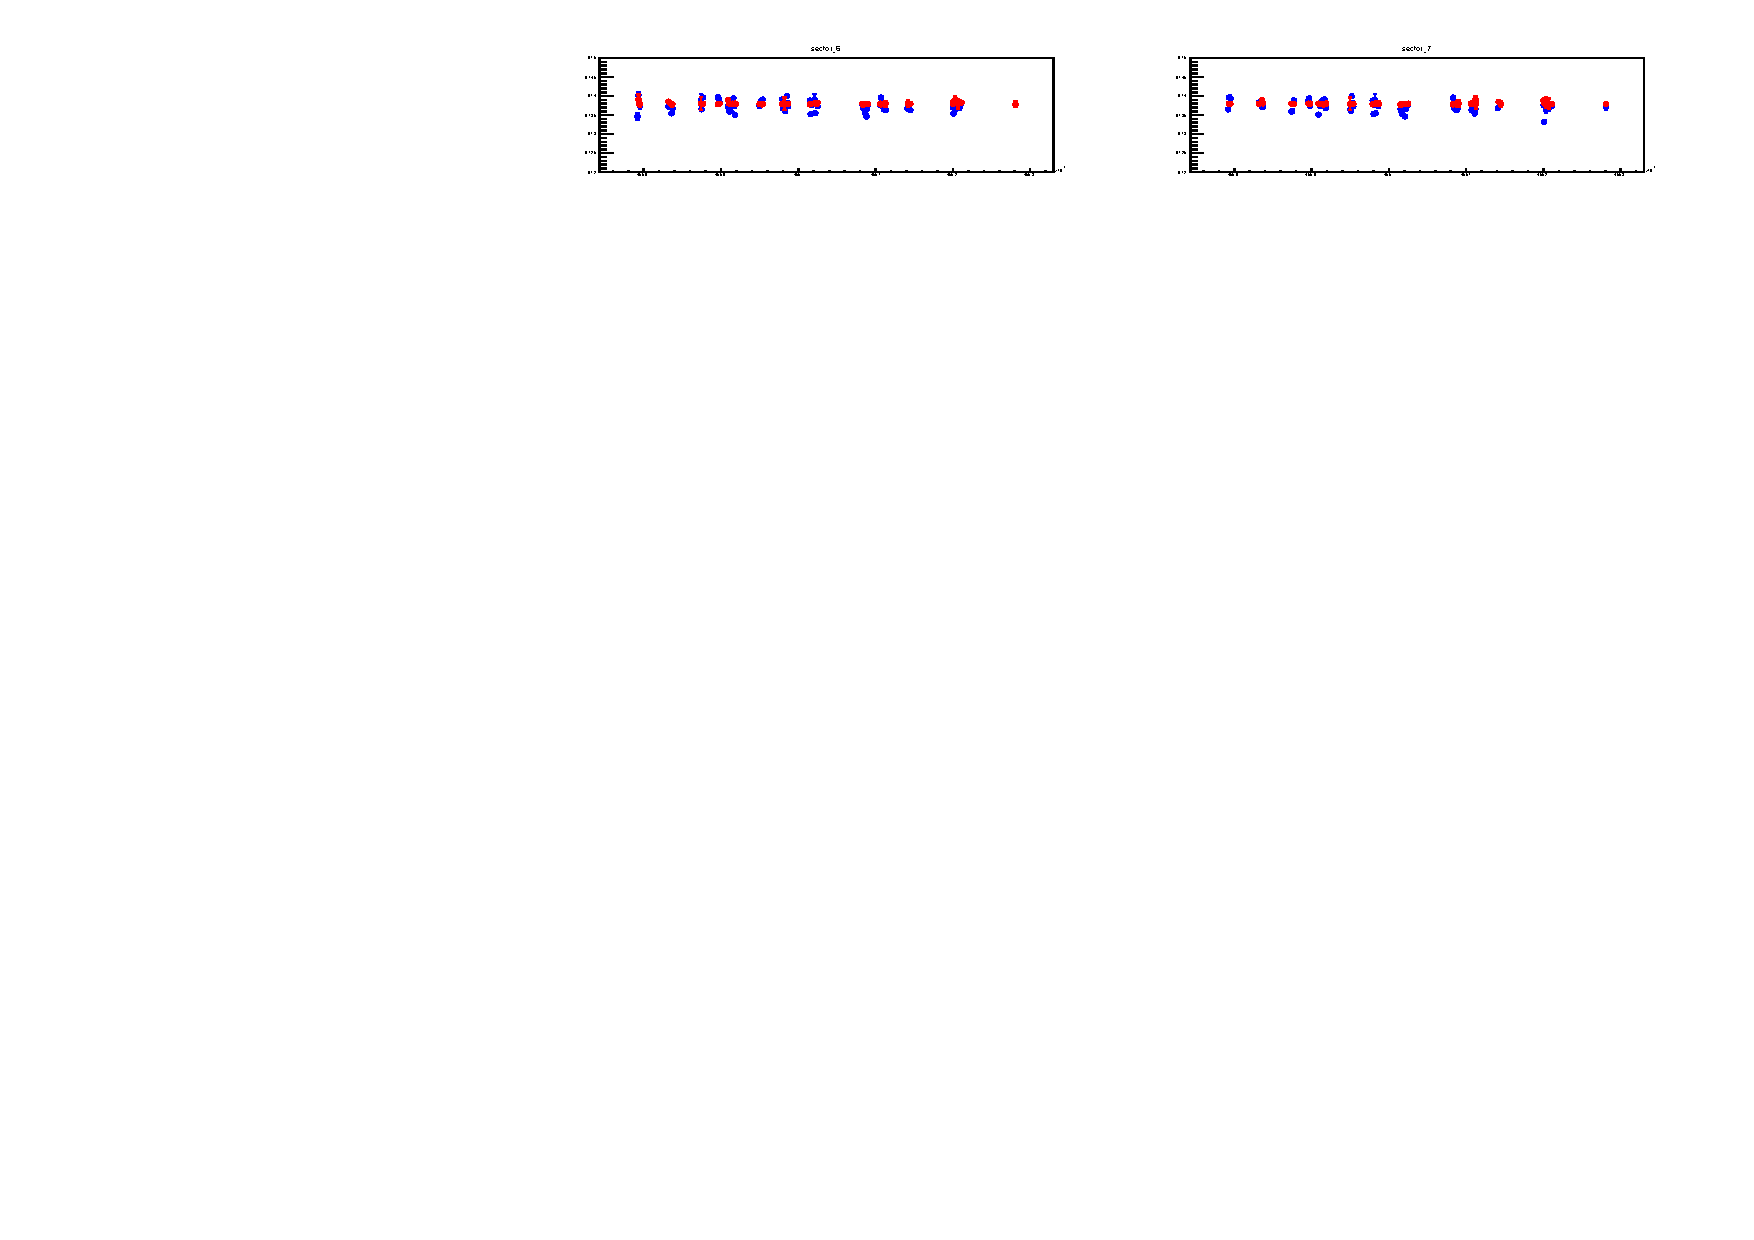
\includegraphics[width=1\textwidth]{fig_pi0vn/nocalib_vs_calib_sect7-8.pdf}
    \caption{dAu 62 GeV, Energy recalibration of PbGl sectors . Mean $\pi^{0}$ peak before(blue) and after(red) calibration for all the runs}
    \label{meanpi0vsrunsect67}
\end{figure}
The figure \ref{sigma62GeV} shows the sigma of the $\pi^{0}$ peak vs pt for sector 1 and sector 6. 
\begin{figure}
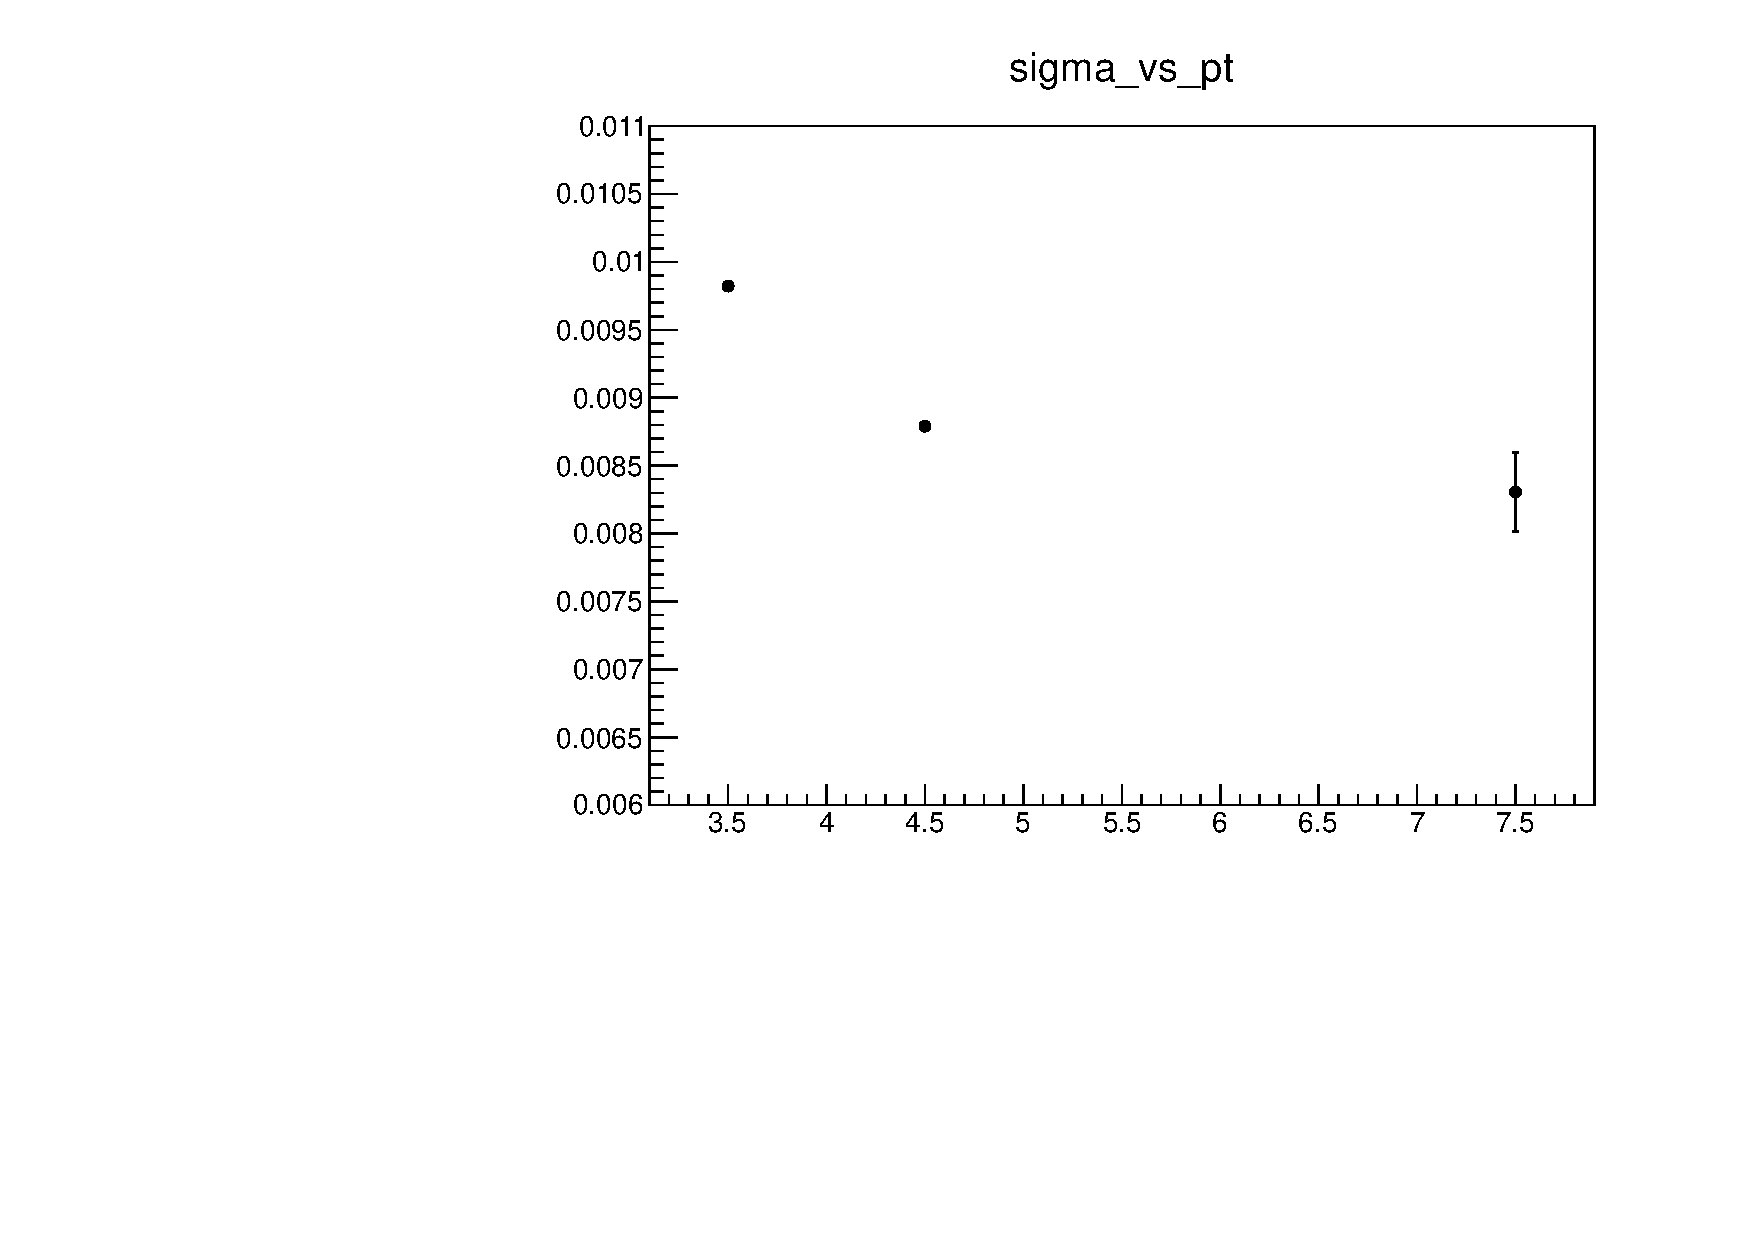
\includegraphics[width=0.47\textwidth]{fig_pi0vn/sect1_sigmavspt62GeV.pdf}
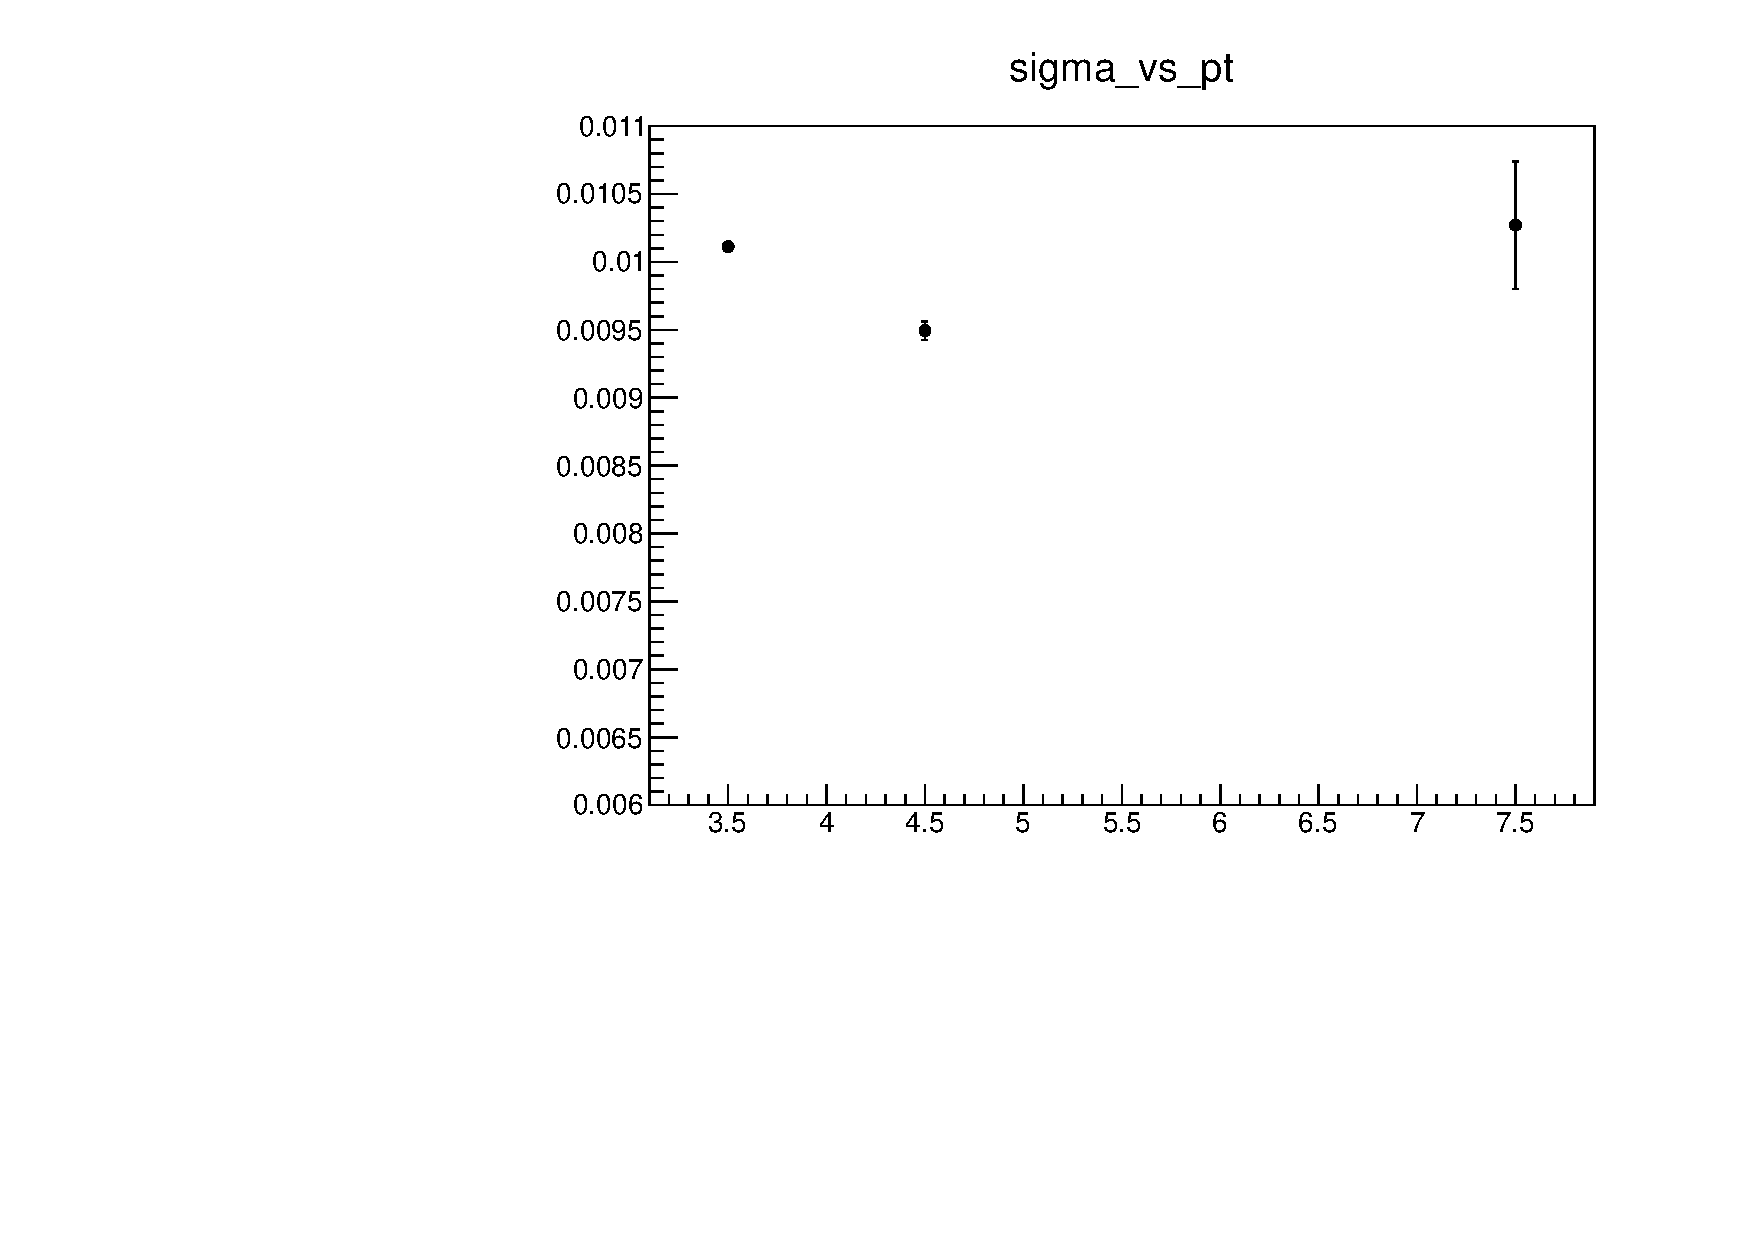
\includegraphics[width=0.47\textwidth]{fig_pi0vn/sect6_sigmavspt62GeV.pdf}
\caption{Sigma of the pi0 peak vs $p_{T}$ for sector 1 (left) and sector 6 (right). $3<p_{T}<10GeV$ , 62 GeV }
\label{sigma62GeV}
\end{figure}
\section{EMCal timing}
\label{section:EMCal timing}
The EMCal towers' TDC can be used to further improve the photon identification and to reduce event pileup.
The procedure to calibrate the TDC signals tower by tower and run by run is well established and well documented in previous analysis notes (CITE ALL).
However the peculiarities on the run conditions make the calibration procedure slightly different for different data sets.
For run 2016, we have adopted a series of five steps in the calibration as follows:

\subsection{One. Find Sector Offset Run by Run}
\begin{figure}
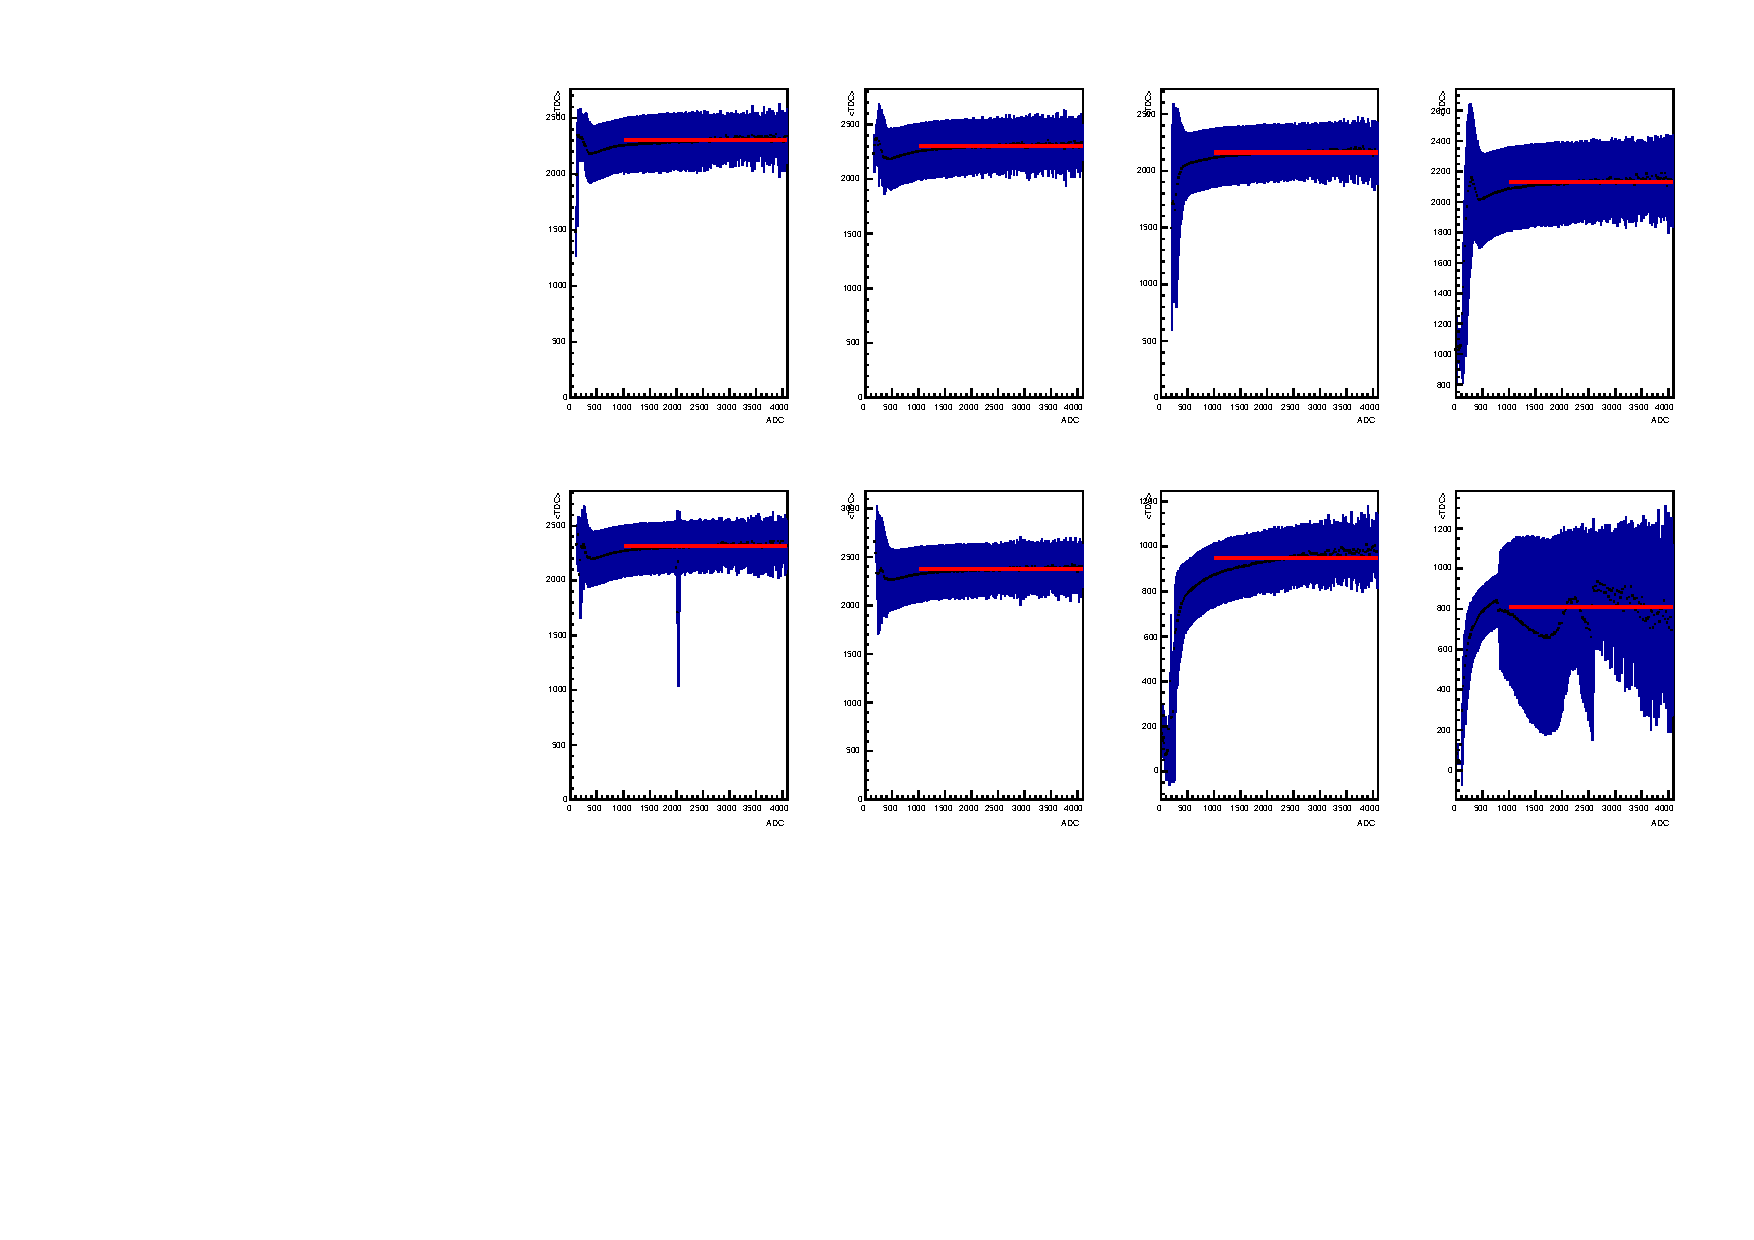
\includegraphics[width=\textwidth]{fig_pi0vn/454800.pdf}
\caption{Timing Step One. Sector offset for run 454800. First six sectors correspond to PbSc; last two, to PbGl.}
\label{fig.tim.one}
\end{figure}
We find the mean TDC signal per ADC channel of all the towers in the same sector and fit the high ADC as seen in figure \ref{fig.tim.one}.
Then we aligned these ranges in a run by run basis to a default value of 2500 TDC units.
\subsection{Two. Find Tower by tower TDC band}
\begin{figure}
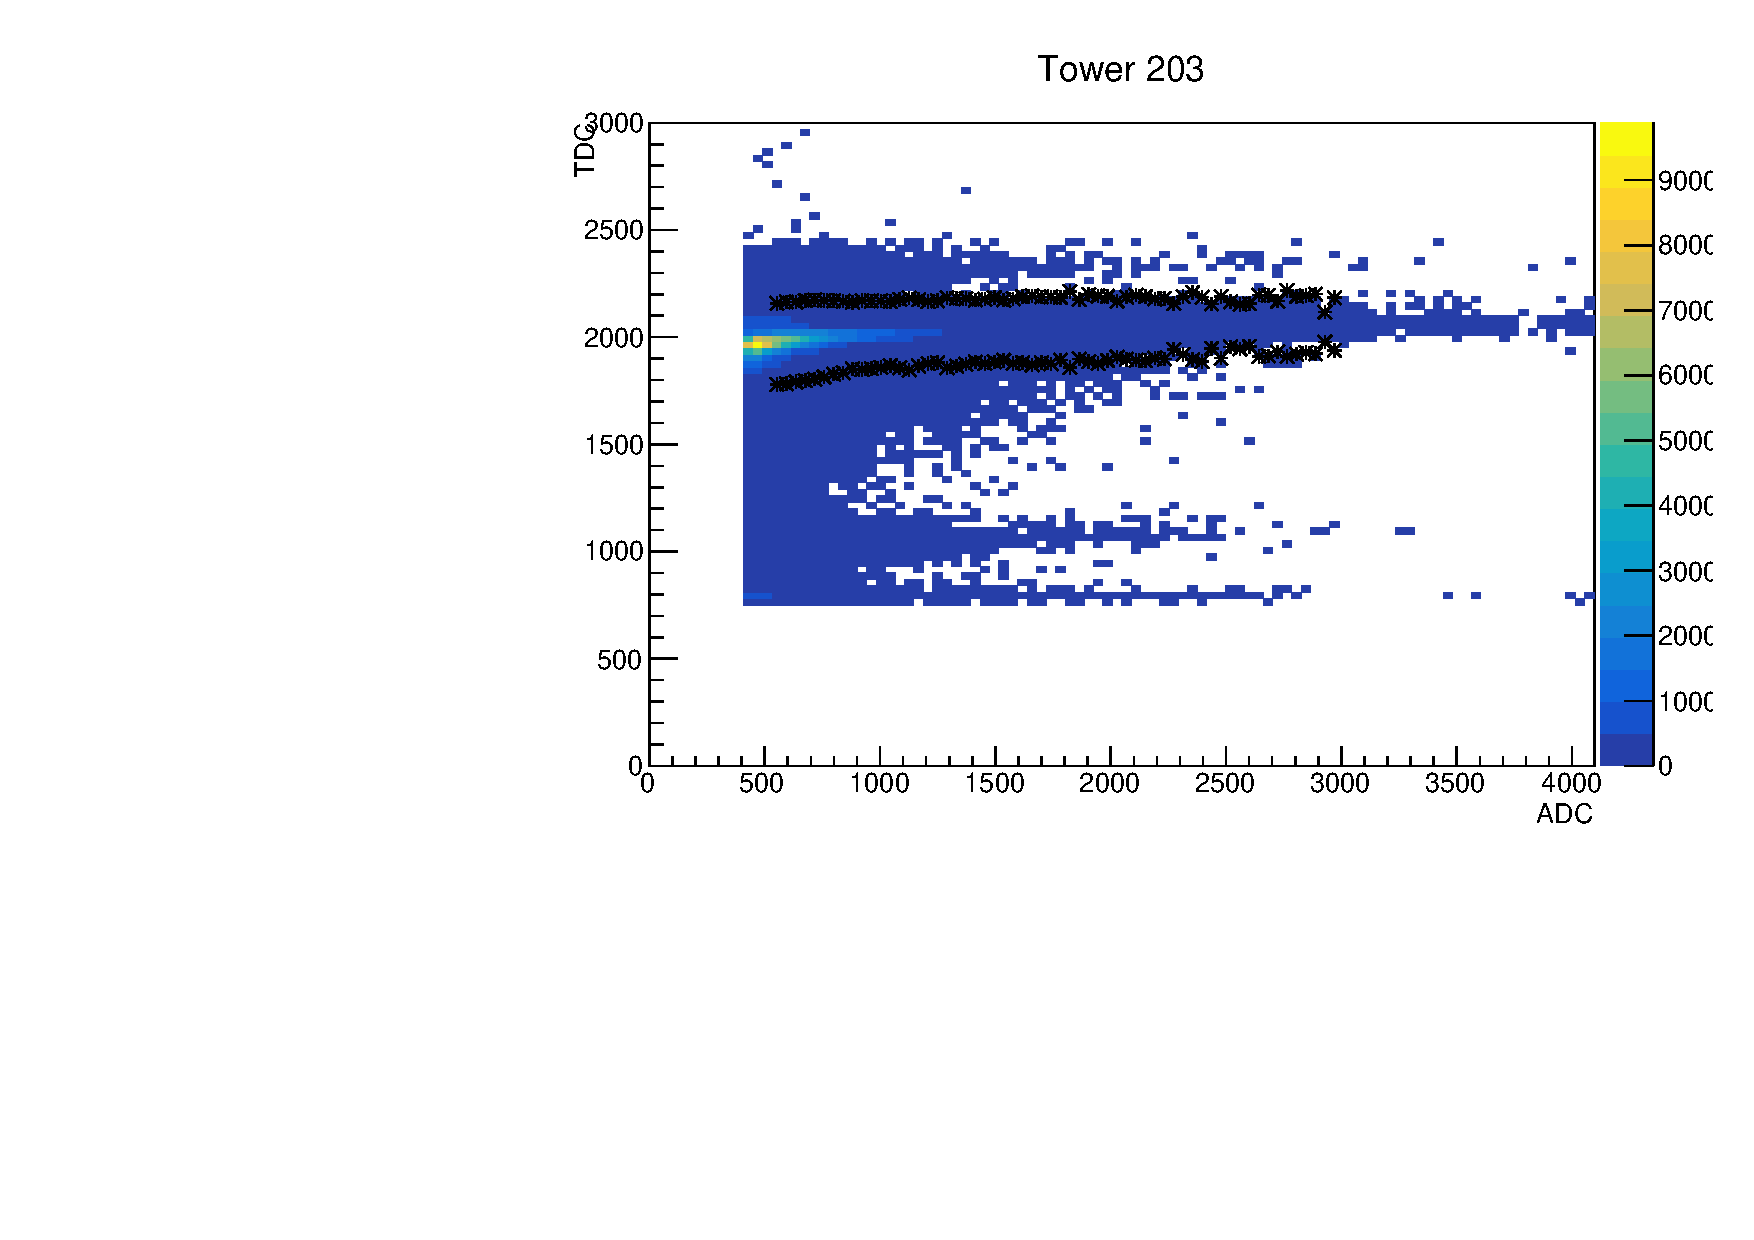
\includegraphics[width=0.47\textwidth]{fig_pi0vn/range_t203.pdf}
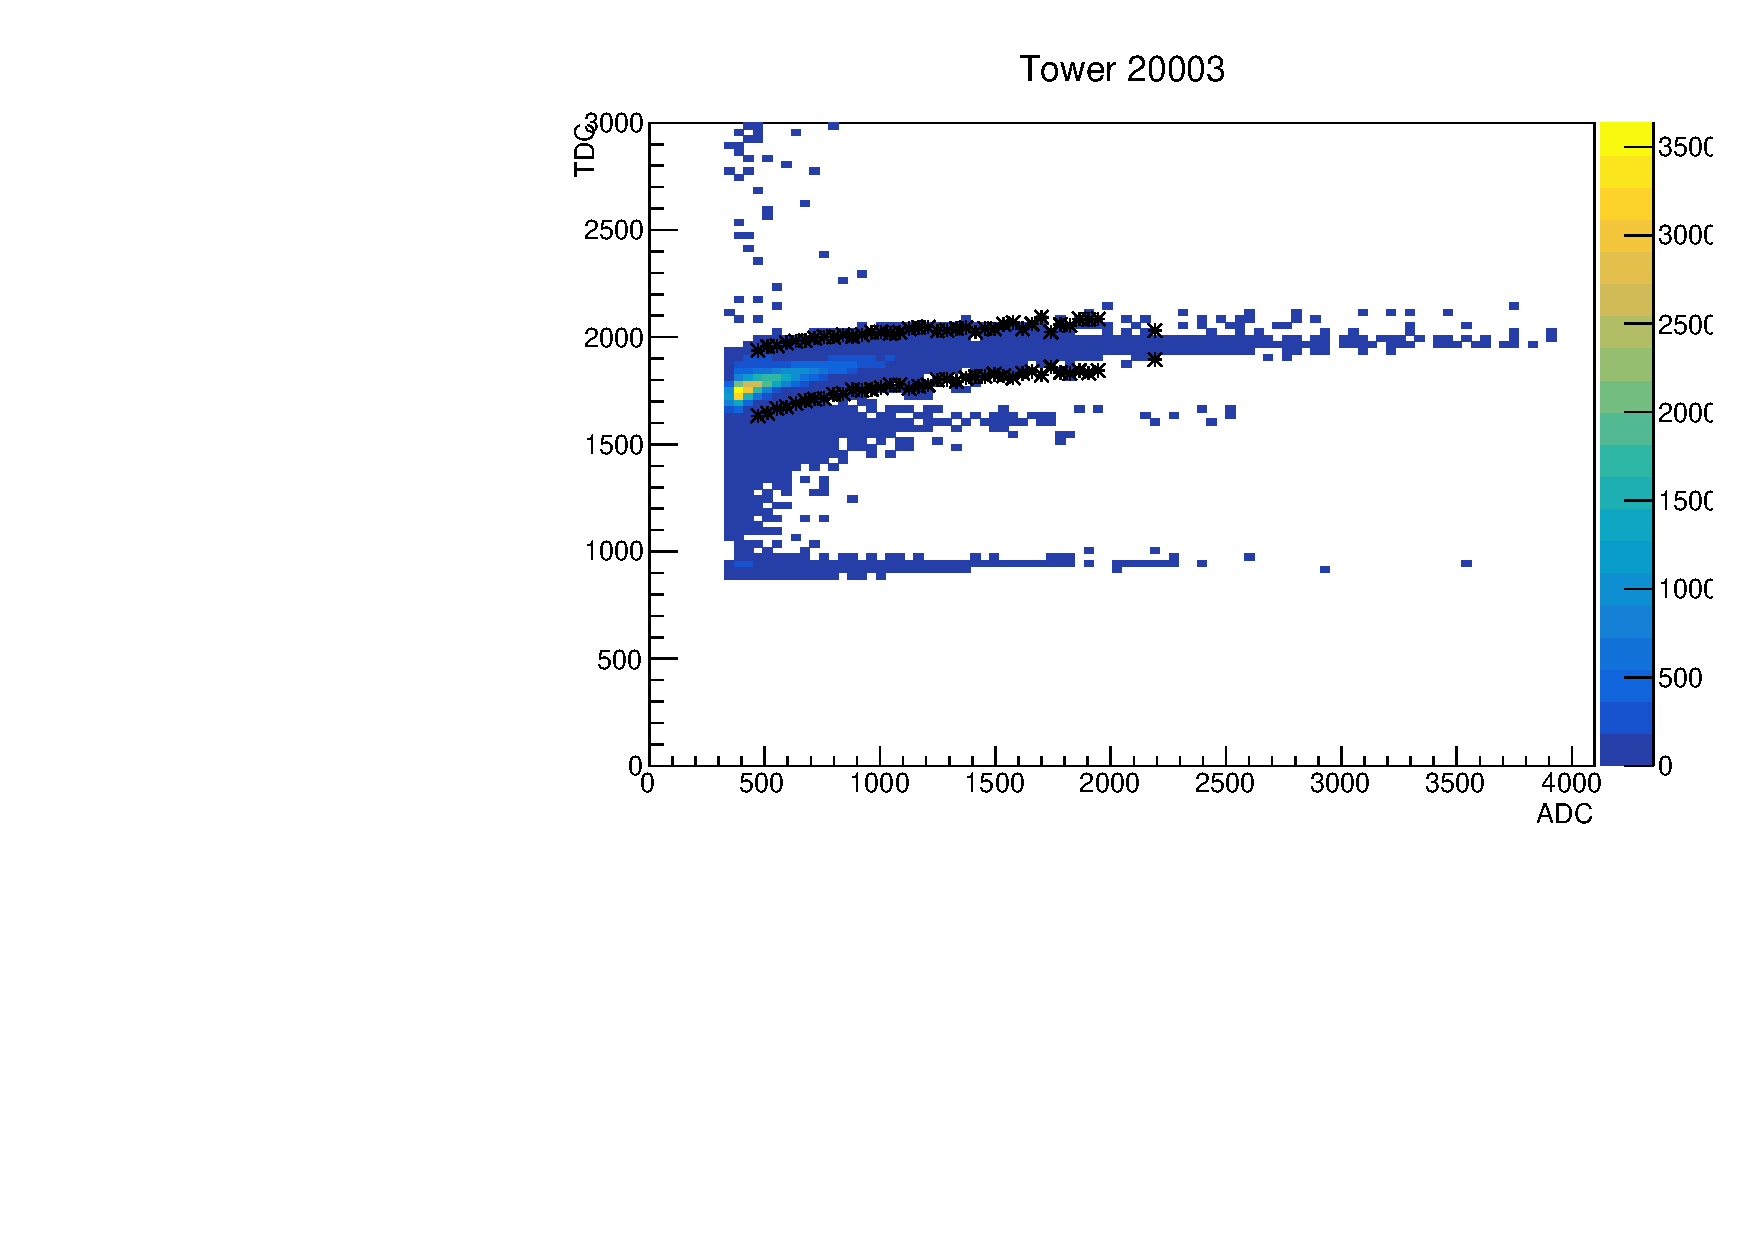
\includegraphics[width=0.47\textwidth]{fig_pi0vn/range_t20003.pdf}
\caption{Timing Step Two. Neighborhood around mode for typical PbSc tower (left) and PbGl tower (right).}
\label{fig.tim.two}
\end{figure}
Once we have aligned the potential run by run variation, we proceed to find a neighborhood around the TDC maxima.
The neighborhood is set up to be 3 RMS above and below the maxima.
The width was chosen based on a previous QA of the pulse shape characteristics for all of the 24768 towers.
A plot related to the found band for a typical tower in PbSc and PbGl is shown in figure \ref{fig.tim.two}.
\subsection{Three. Find Maxima with good accuracy}
\begin{figure}
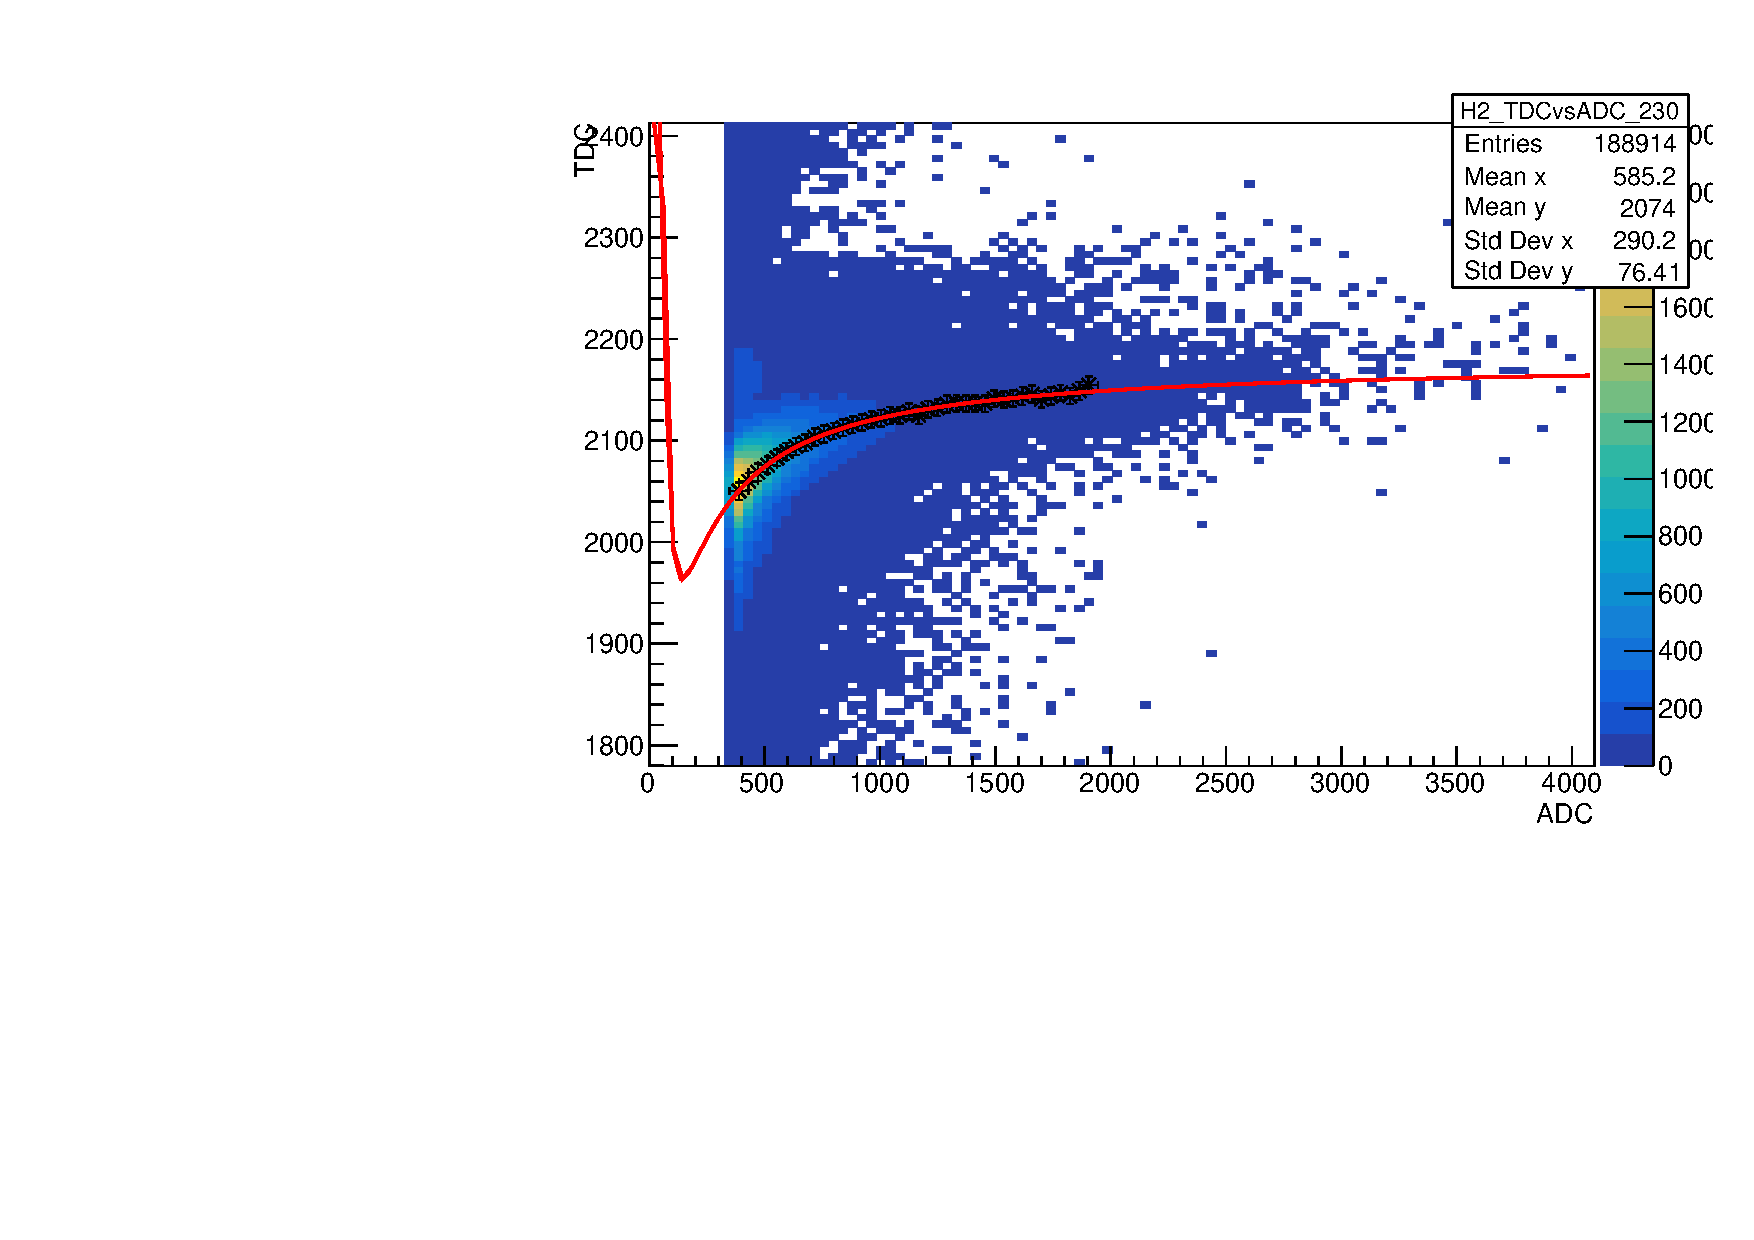
\includegraphics[width=0.47\textwidth]{fig_pi0vn/mode_t230.pdf}
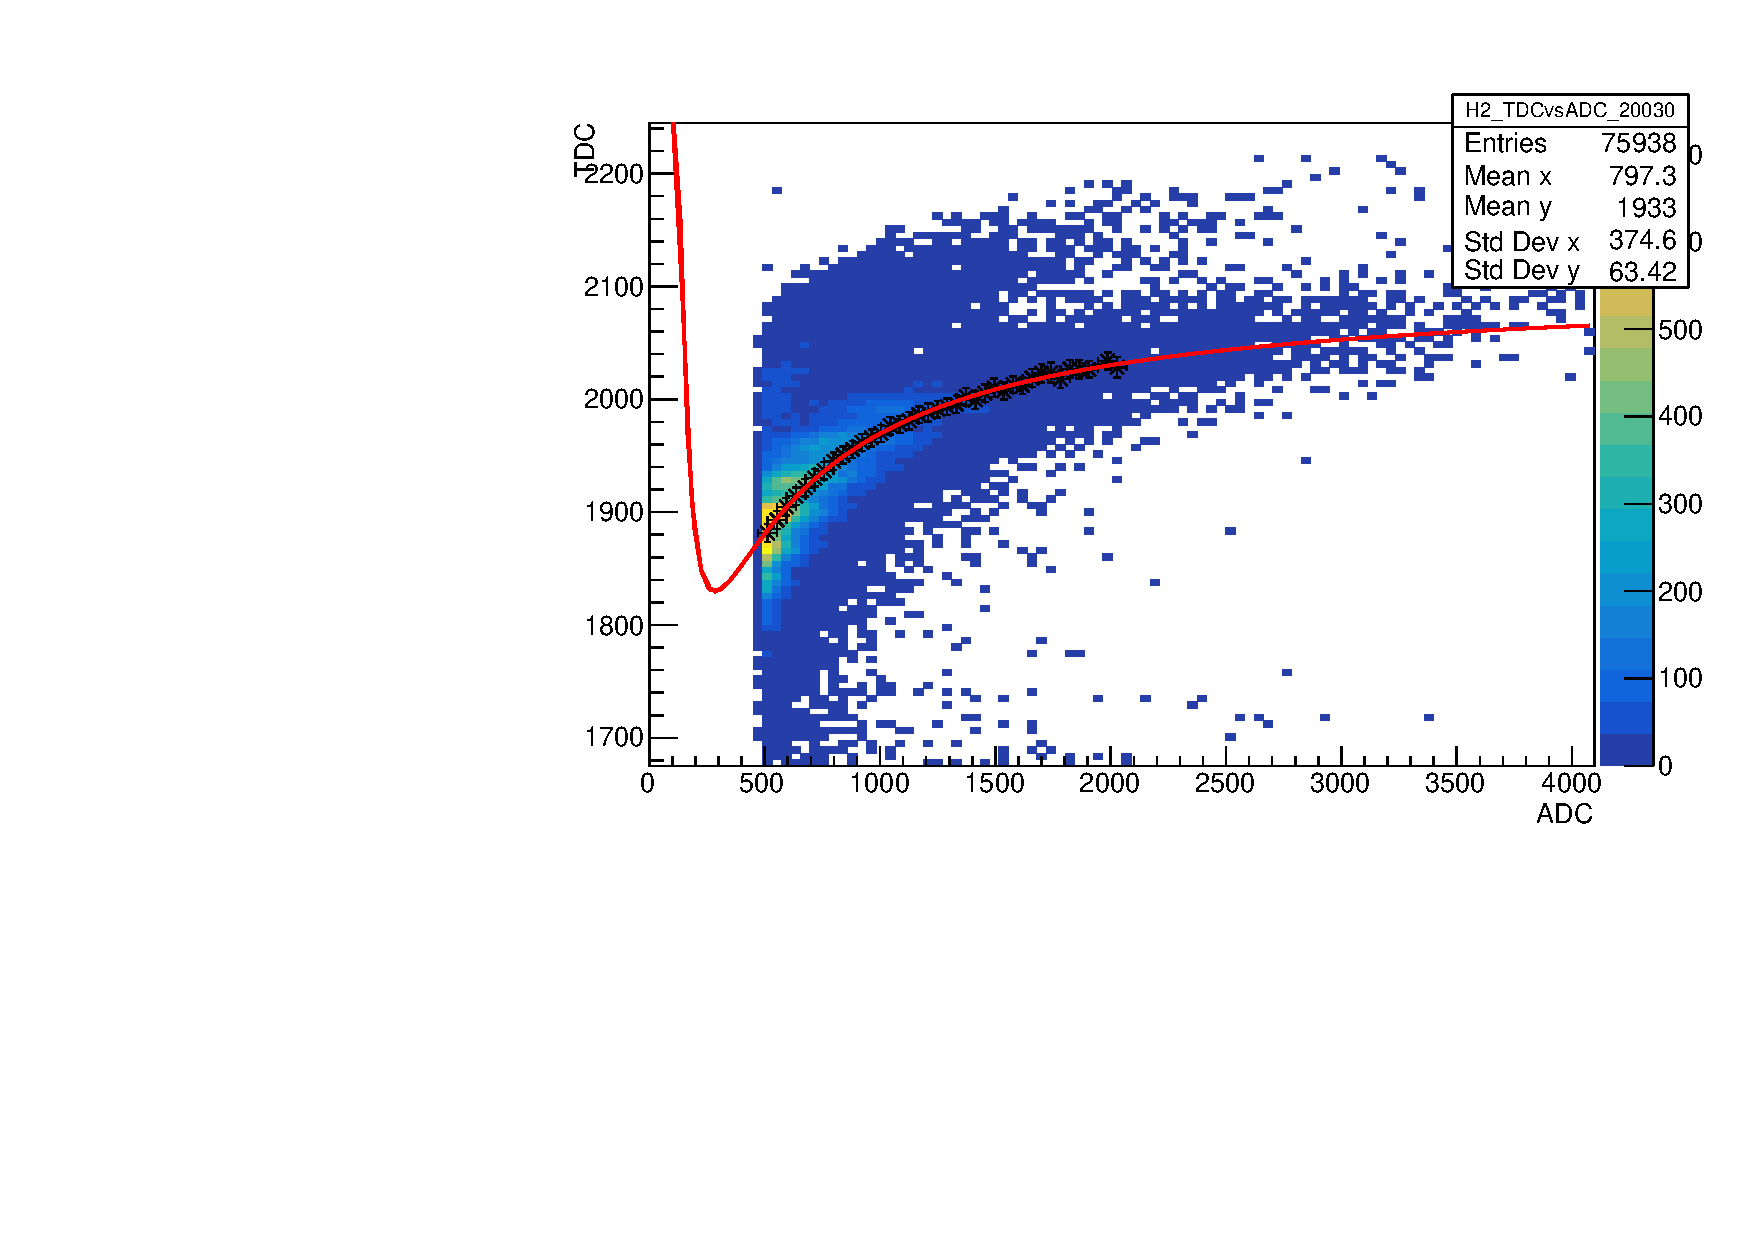
\includegraphics[width=0.47\textwidth]{fig_pi0vn/mode_t20030.pdf}
\caption{Timing Step Three. Finding mode in typical PbSc tower (left) and PbGl tower (right).}
\label{fig.tim.three}
\end{figure}
Once the analysis band is set up, we histogram the TDC vs ADC response with fine binning.
Then we find the mode of the TDC distribution per ADC bin by looking up recursively in the TDC-projection of the histogram.
Five iteration are enough to find a stable value for the mode and the error in estimation.
Figure \ref{fig.tim.three} shows a two dimensional histogram of the TDC vs ADC together with both the data that corresponds to the TDC mode as a function of ADC and its fit to a characteristic function.
The function used to quantify the slewing is: $[0]+[1]/x+[2]/x^2$, where the last term corrects for non linearity found for the lowest ADC signals.

\subsection{Four. Building TOF}
Next We build the TOF for the towers.
The following expression is used:
$$TOF^{'}(tower) = A*(TDC(tower)-s_1/x-S_2/x^2) - d(clus-vtx)/c - T_{0}$$
, where:
\begin{itemize}
\item{A} is a factor that converts TDC units to ns
\item{d(clus-vtx)} is the distance between the central tower if the cluster and the vertex
\item$T_{0}$ is the lapse between the interaction clock and the BBC timing. Notice that EMC TDC measures with respect to the interaction clock and therefore this subtraction is necessary.
\end{itemize}
\subsection{Five. Aligning TOF for photons to zero}
\begin{figure}
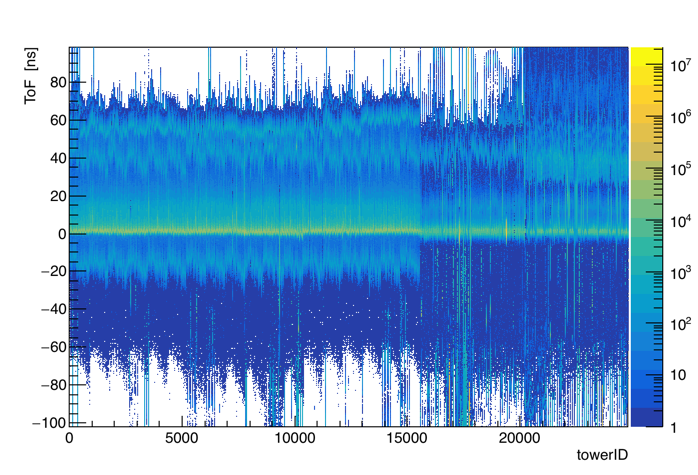
\includegraphics[width=\textwidth]{fig_pi0vn/TOF.png}
\caption{Timing Step Five. TOF distribution per tower after run by run alignment. No tower by tower offset yet.}
\label{fig.tim.five.one}
\end{figure}
\begin{figure}
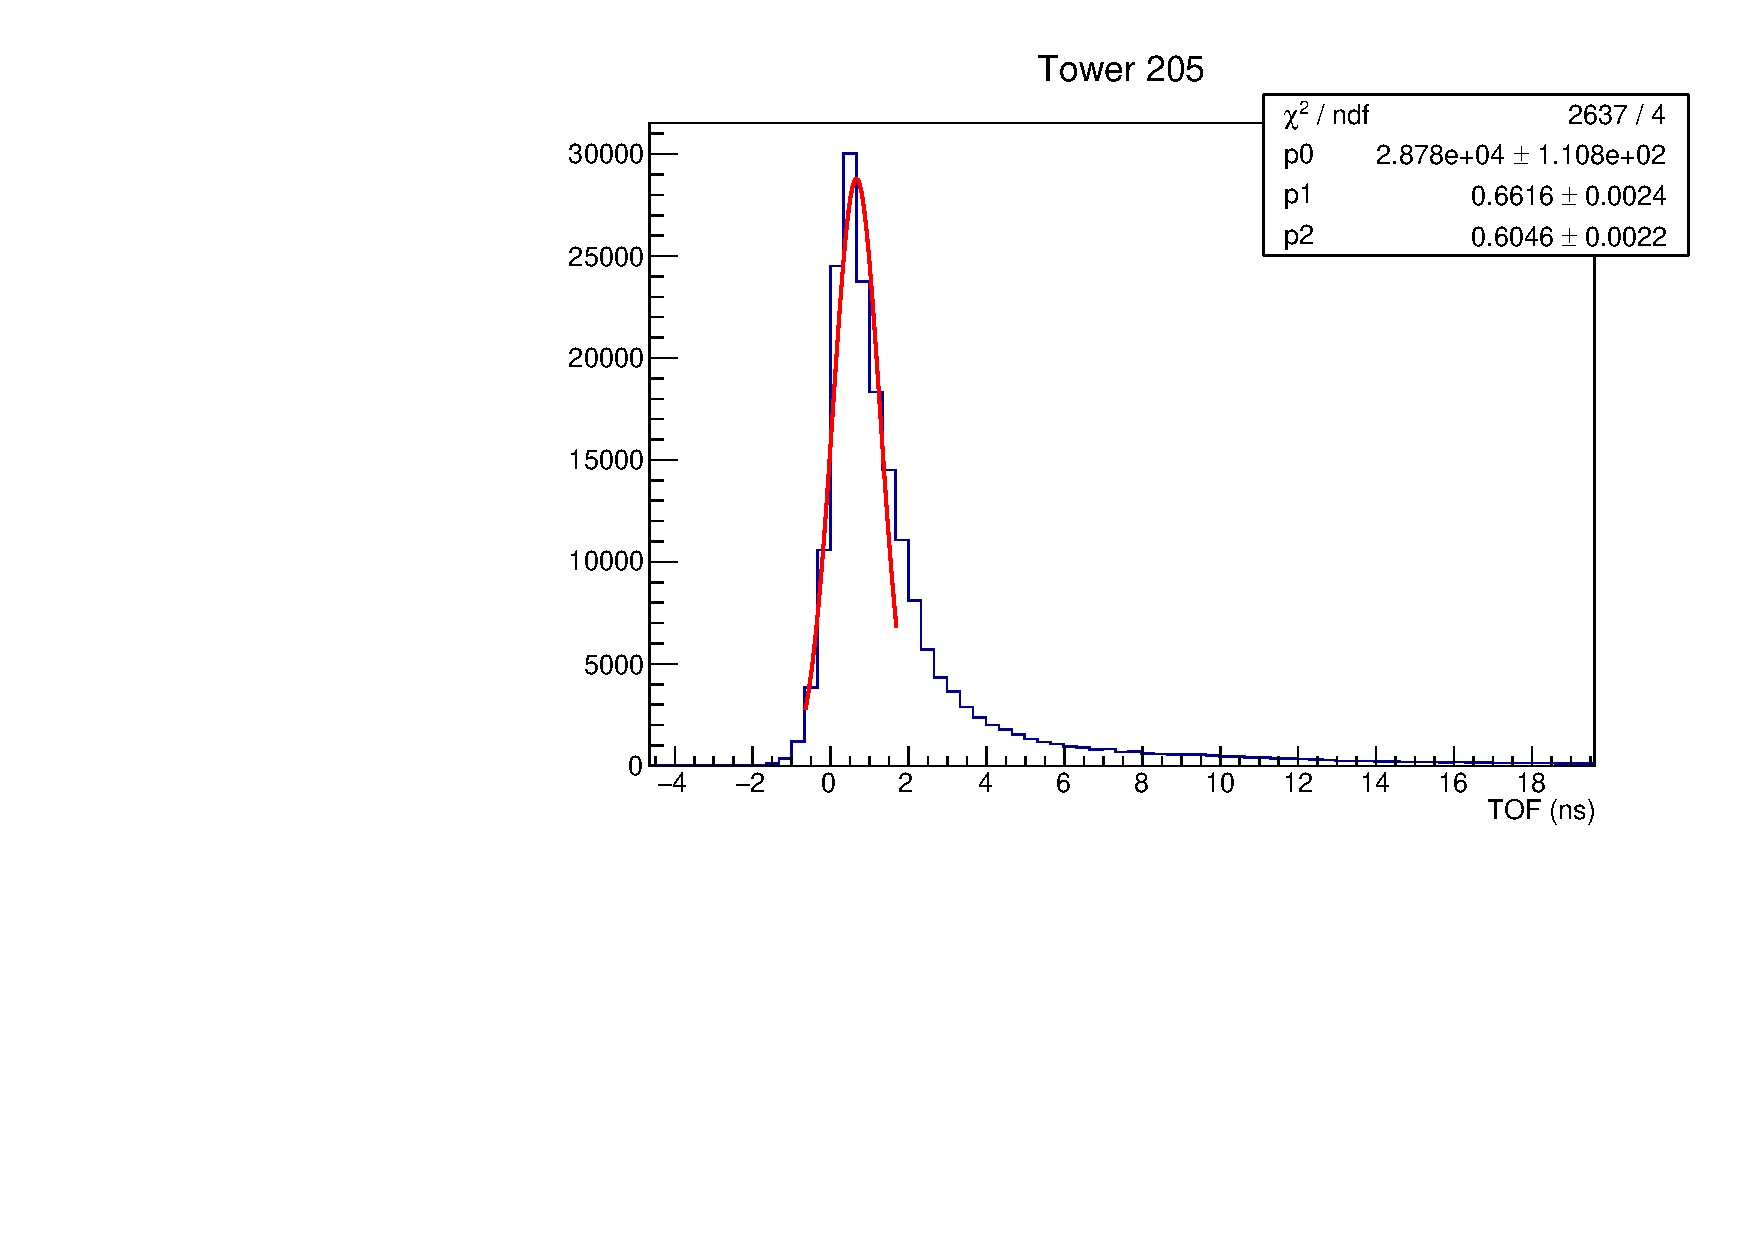
\includegraphics[width=0.47\textwidth]{fig_pi0vn/TOF_t205.pdf}
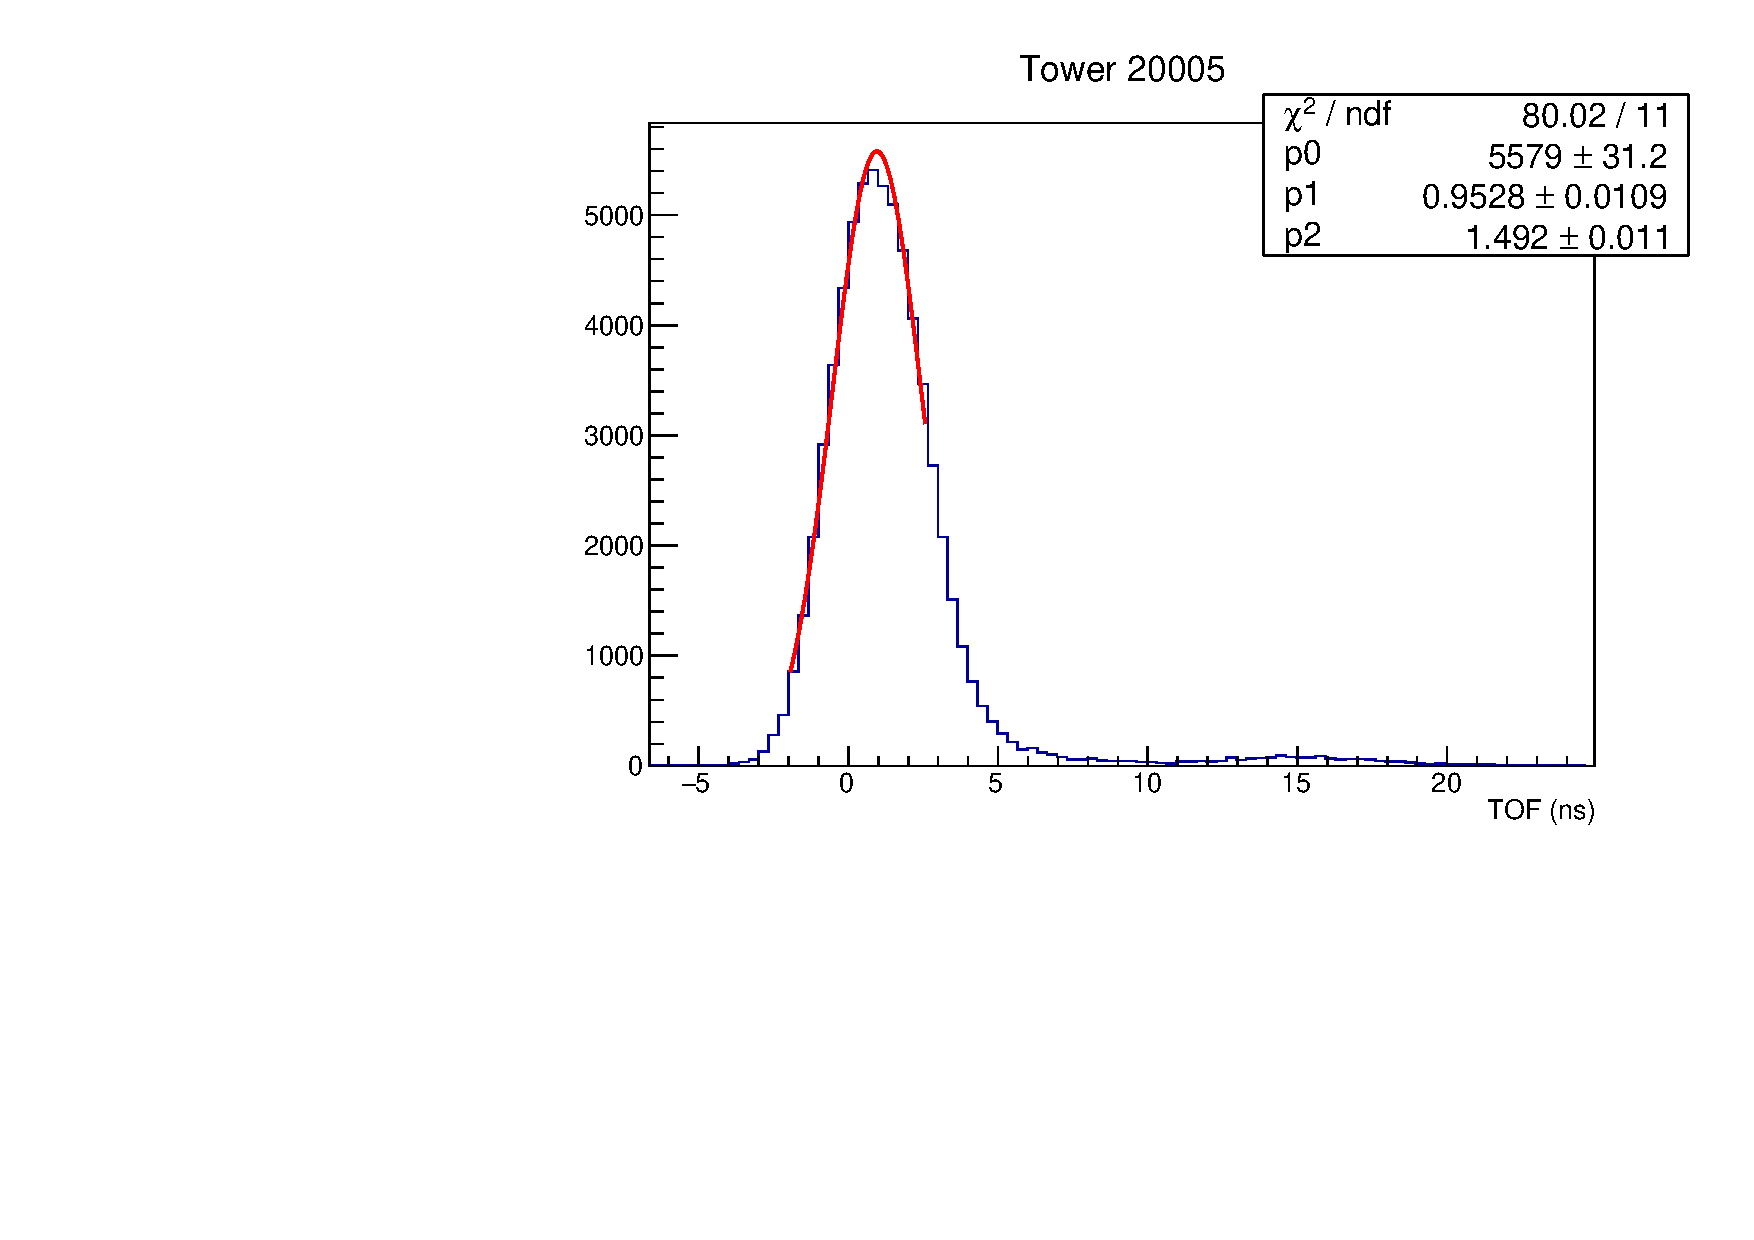
\includegraphics[width=0.47\textwidth]{fig_pi0vn/TOF_t20005.pdf}
\caption{Timing Step Five. Typical pulse shape for PbSc tower (left) and PbGl tower (right).}
\label{fig.tim.five.two}
\end{figure}
\begin{figure}
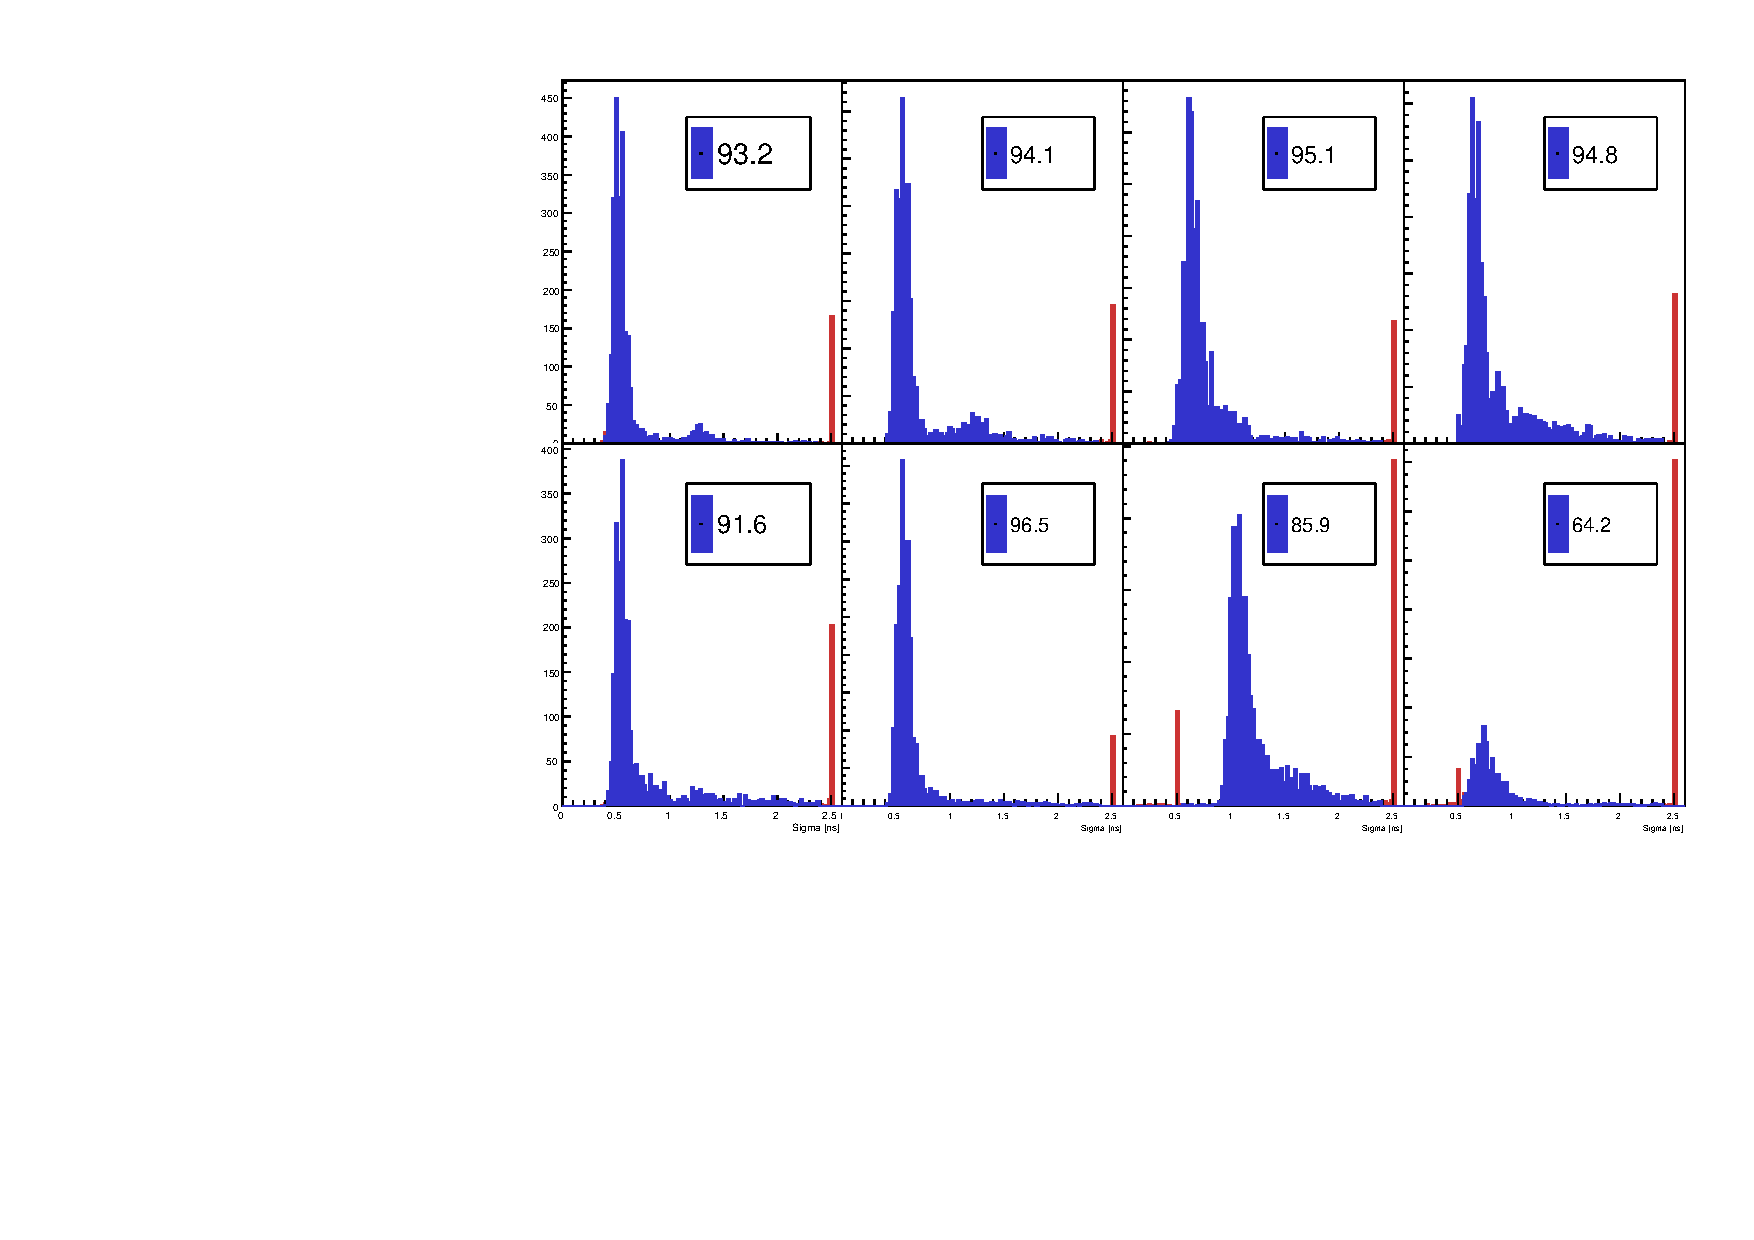
\includegraphics[width=\textwidth]{fig_pi0vn/sigmaTOF.pdf}
\caption{Timing Step Five. Distribution of sigma (ns) of fitted tower pulse shape using Gaussian distribution. Each pad correspond to each sector. Percentage of "healthy" shapes are written in legends.}
\label{fig.tim.five.three}
\end{figure}
After that we compute run by run and tower by tower offsets to put all of the towers TOF to zero for the hypothesis of photons.

$$TOF(tower) = TOF^{'}(tower) - O_1(sector,run) - O_2(tower)$$

Figure \ref{fig.tim.five.one} shows the TOF distribution per tower after the calibration and alignment procedure.
Figure \ref{fig.tim.five.two} shows the pulse shape of a couple of typical towers one for PbSc and one for PbGl. The shapes were fitted to a Gaussian distribution (even though we know that they are not Gaussian) to extract an estimate of the resolution per tower.
Figure \ref{fig.tim.five.three} shows the resolution obtained for each of the towers per sector. As one can see, the typical resolution is at about 600ps for PbSc and 1.5ns for PbGl.
\begin{figure}
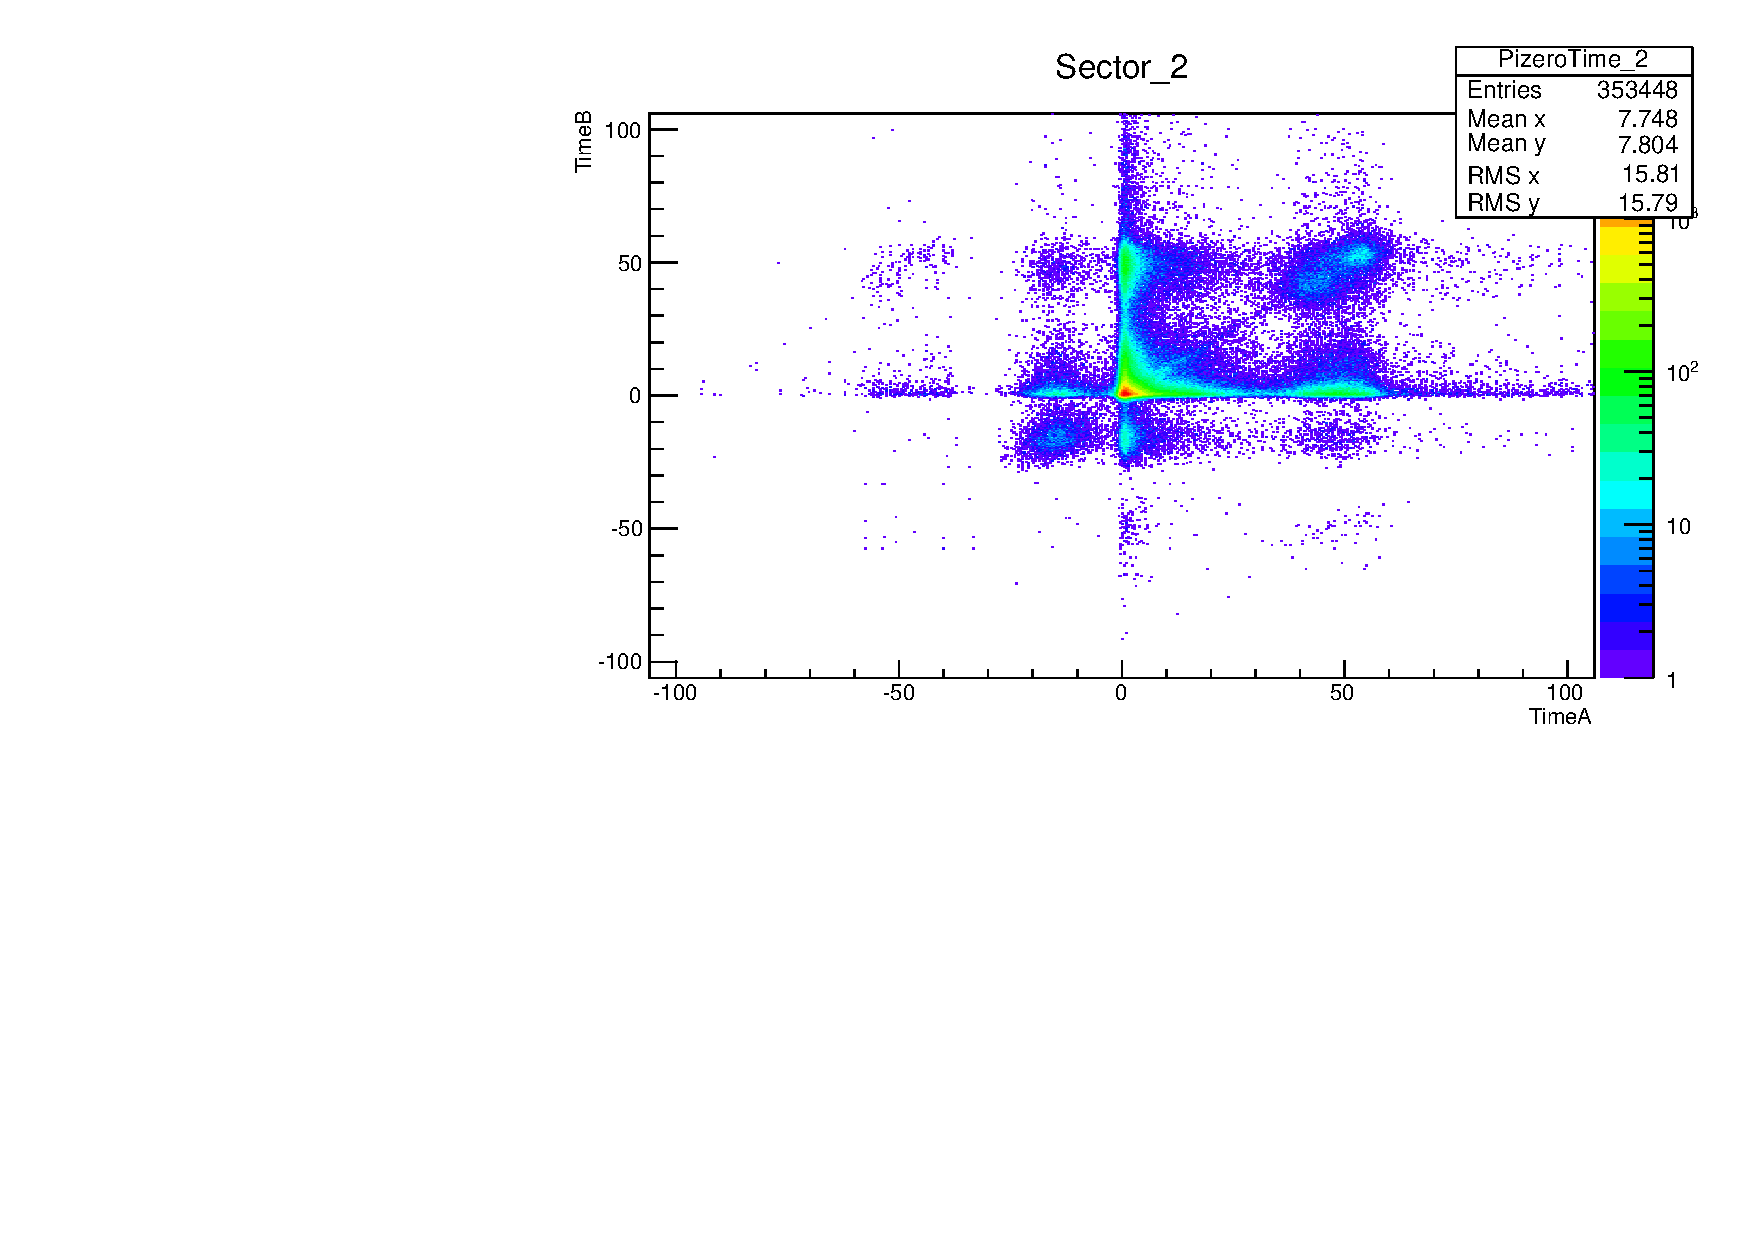
\includegraphics[width=\textwidth]{fig_pi0vn/clustert1_clustert2_sect2.pdf}
\caption{EMC Timing distribution of a pair of clusters. Most clusters are around 0ns and additional peak apears around 50ns}
\label{cluster1vscluster2}
\end{figure}
In figure \ref{cluster1vscluster2} we show the timing distribution of the cluster pairs for a $\pi^0->\gamma+\gamma$. We can see the overlapping events. This was studied already in pAu 200GeV 2015 citeautor{norbert2015an1269}.
We can studied the correlation of the two cluster in different regions:
\begin{itemize}
\item{Cut 1: $|t1|<1 ns$ ,$|t2|<1 ns$}
\item{Cut 2: $|t1|<1 ns$ ,$25 <t2<60 ns$}
\item{Cut 3: $25 <t1<60 ns$, $|t2|<1 ns$}
\item{Cut 4: $25 <t1<50 ns$, $25<t2<50 ns$}
\item{Cut 5: $50 <t1<70 ns$, $50<t2<70 ns$}
\end{itemize}
Now , we can reconstruct the invariant mass for each cut.Look at figure \ref{invmasscuts}
\begin{figure}
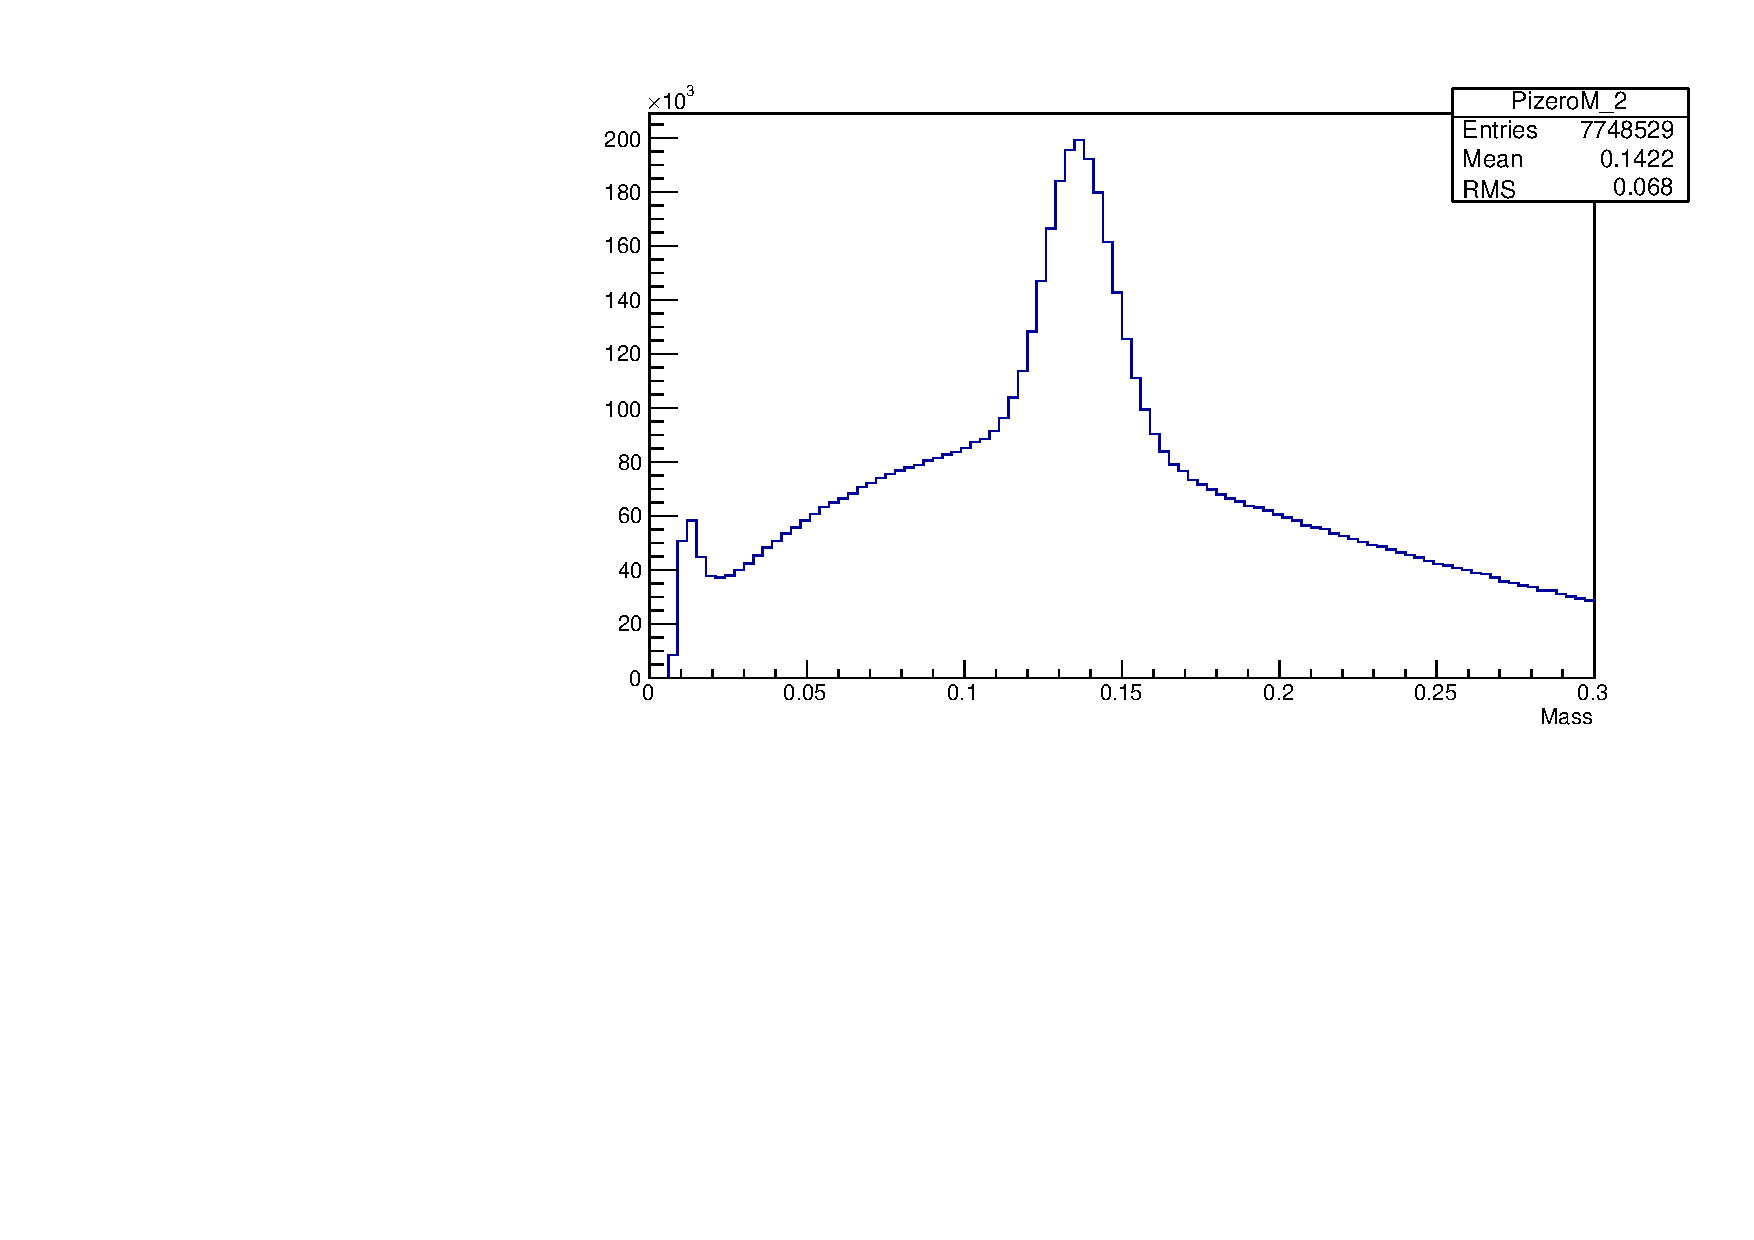
\includegraphics[width=0.47\textwidth]{fig_pi0vn/cut1_sect2allruns.pdf}
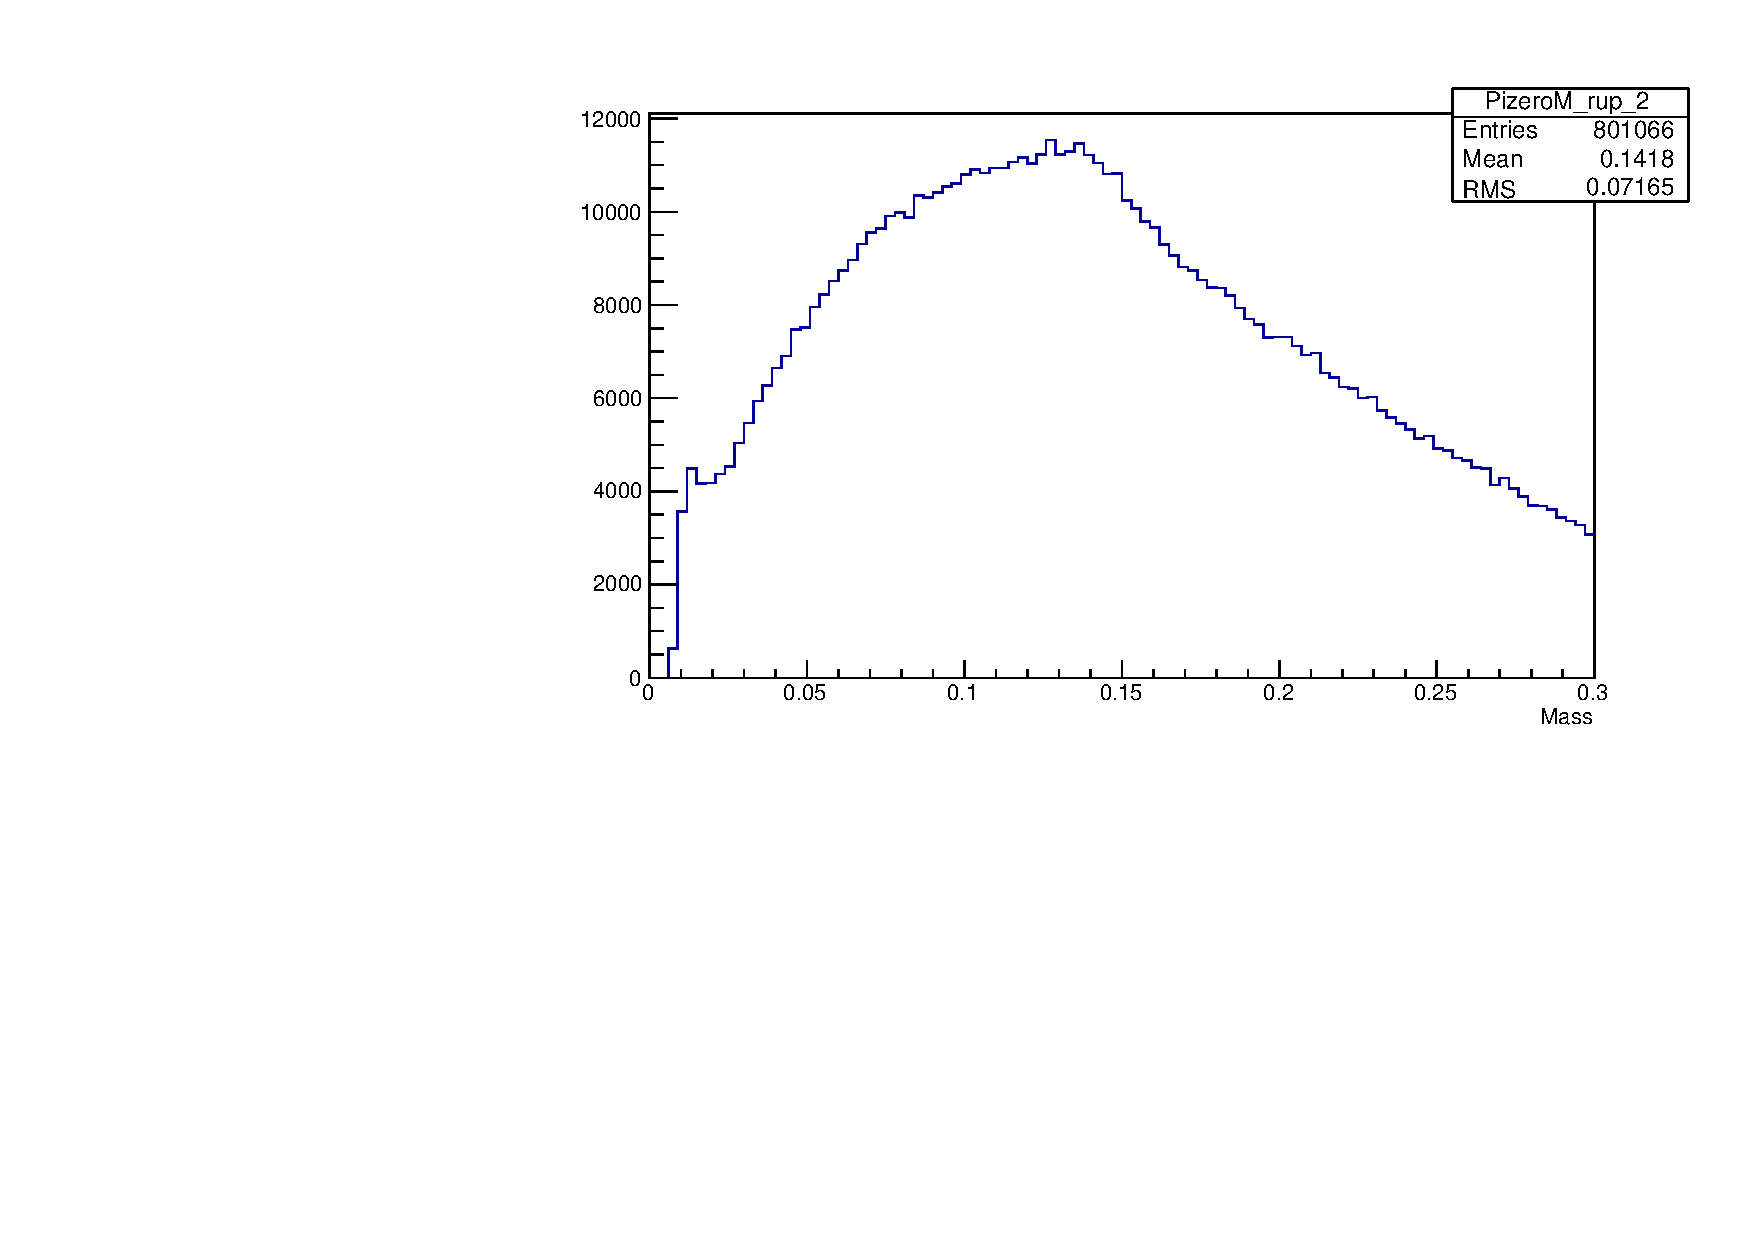
\includegraphics[width=0.47\textwidth]{fig_pi0vn/cut2_sect2allruns.pdf}
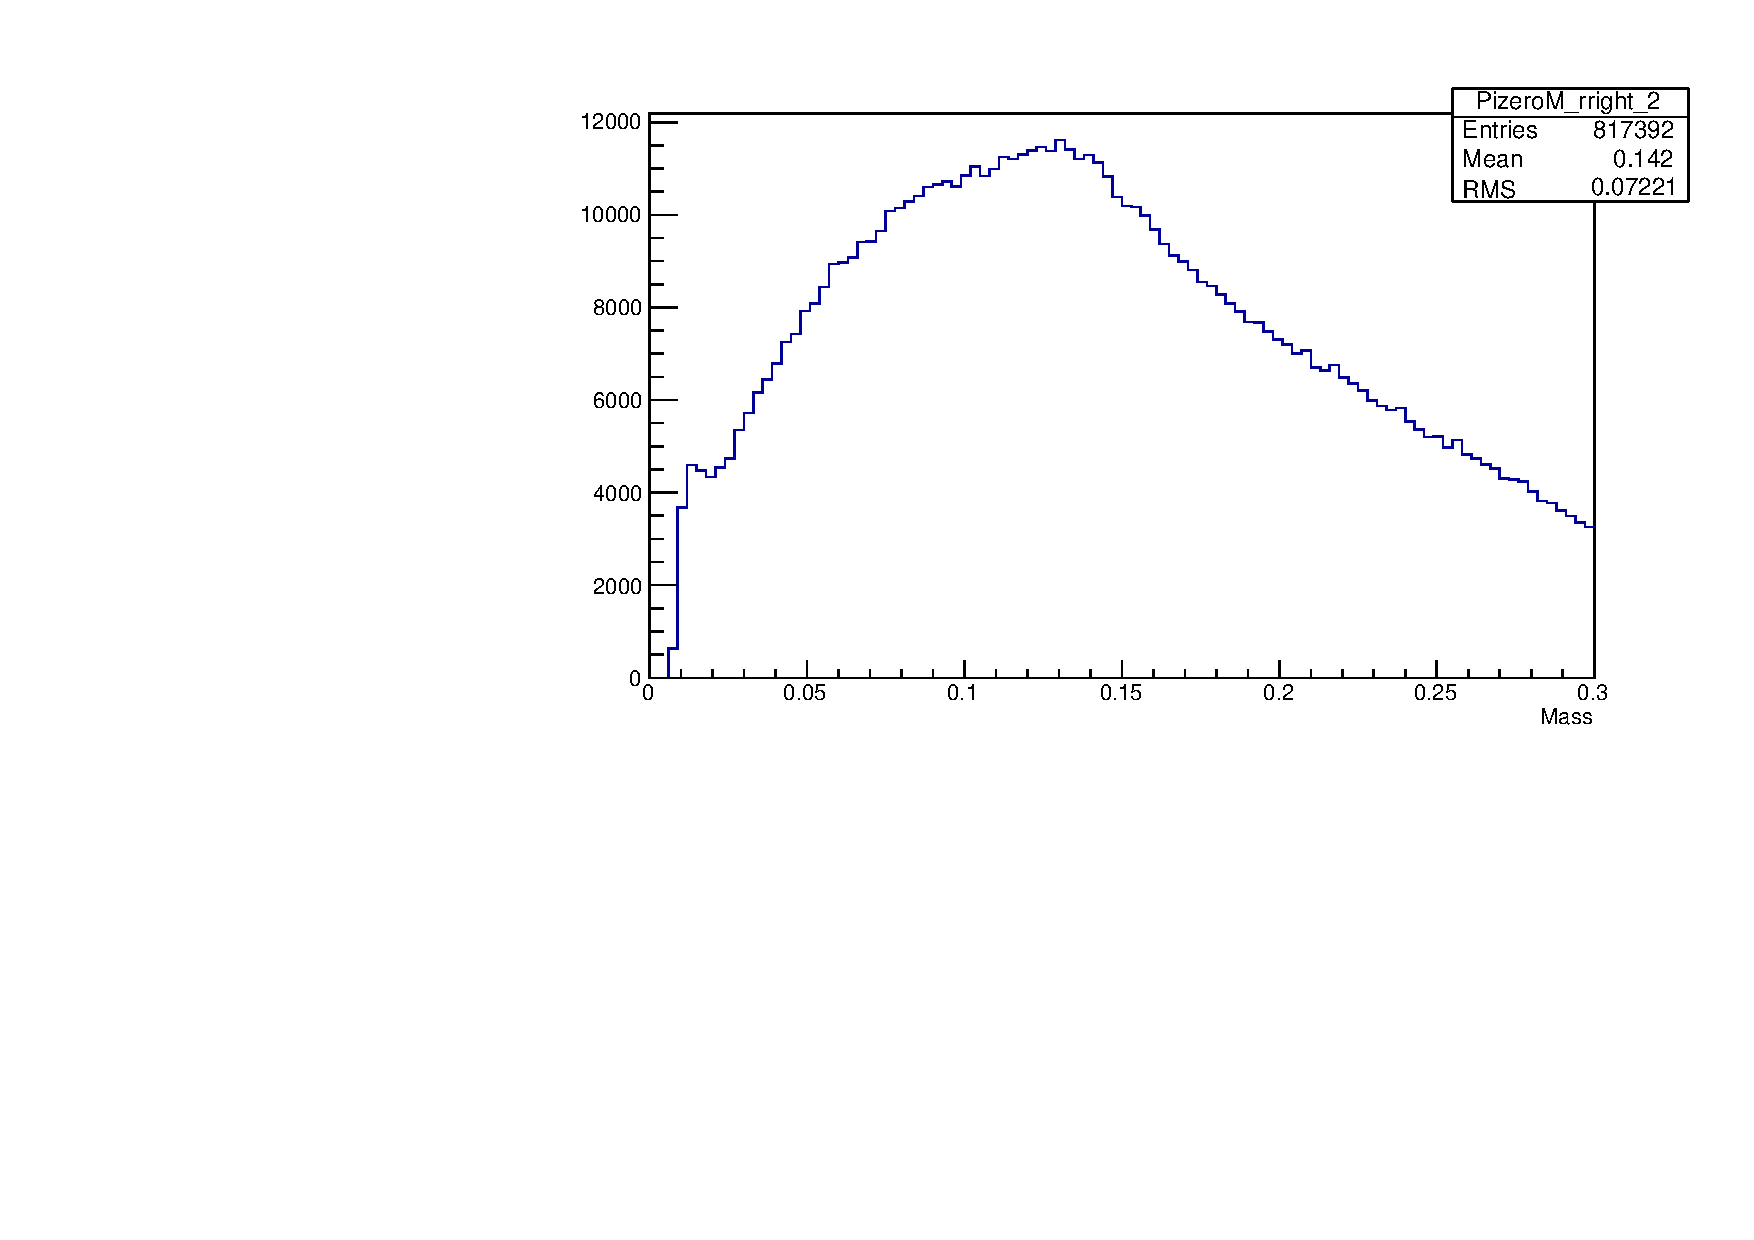
\includegraphics[width=0.47\textwidth]{fig_pi0vn/cut3_sect2allruns.pdf}
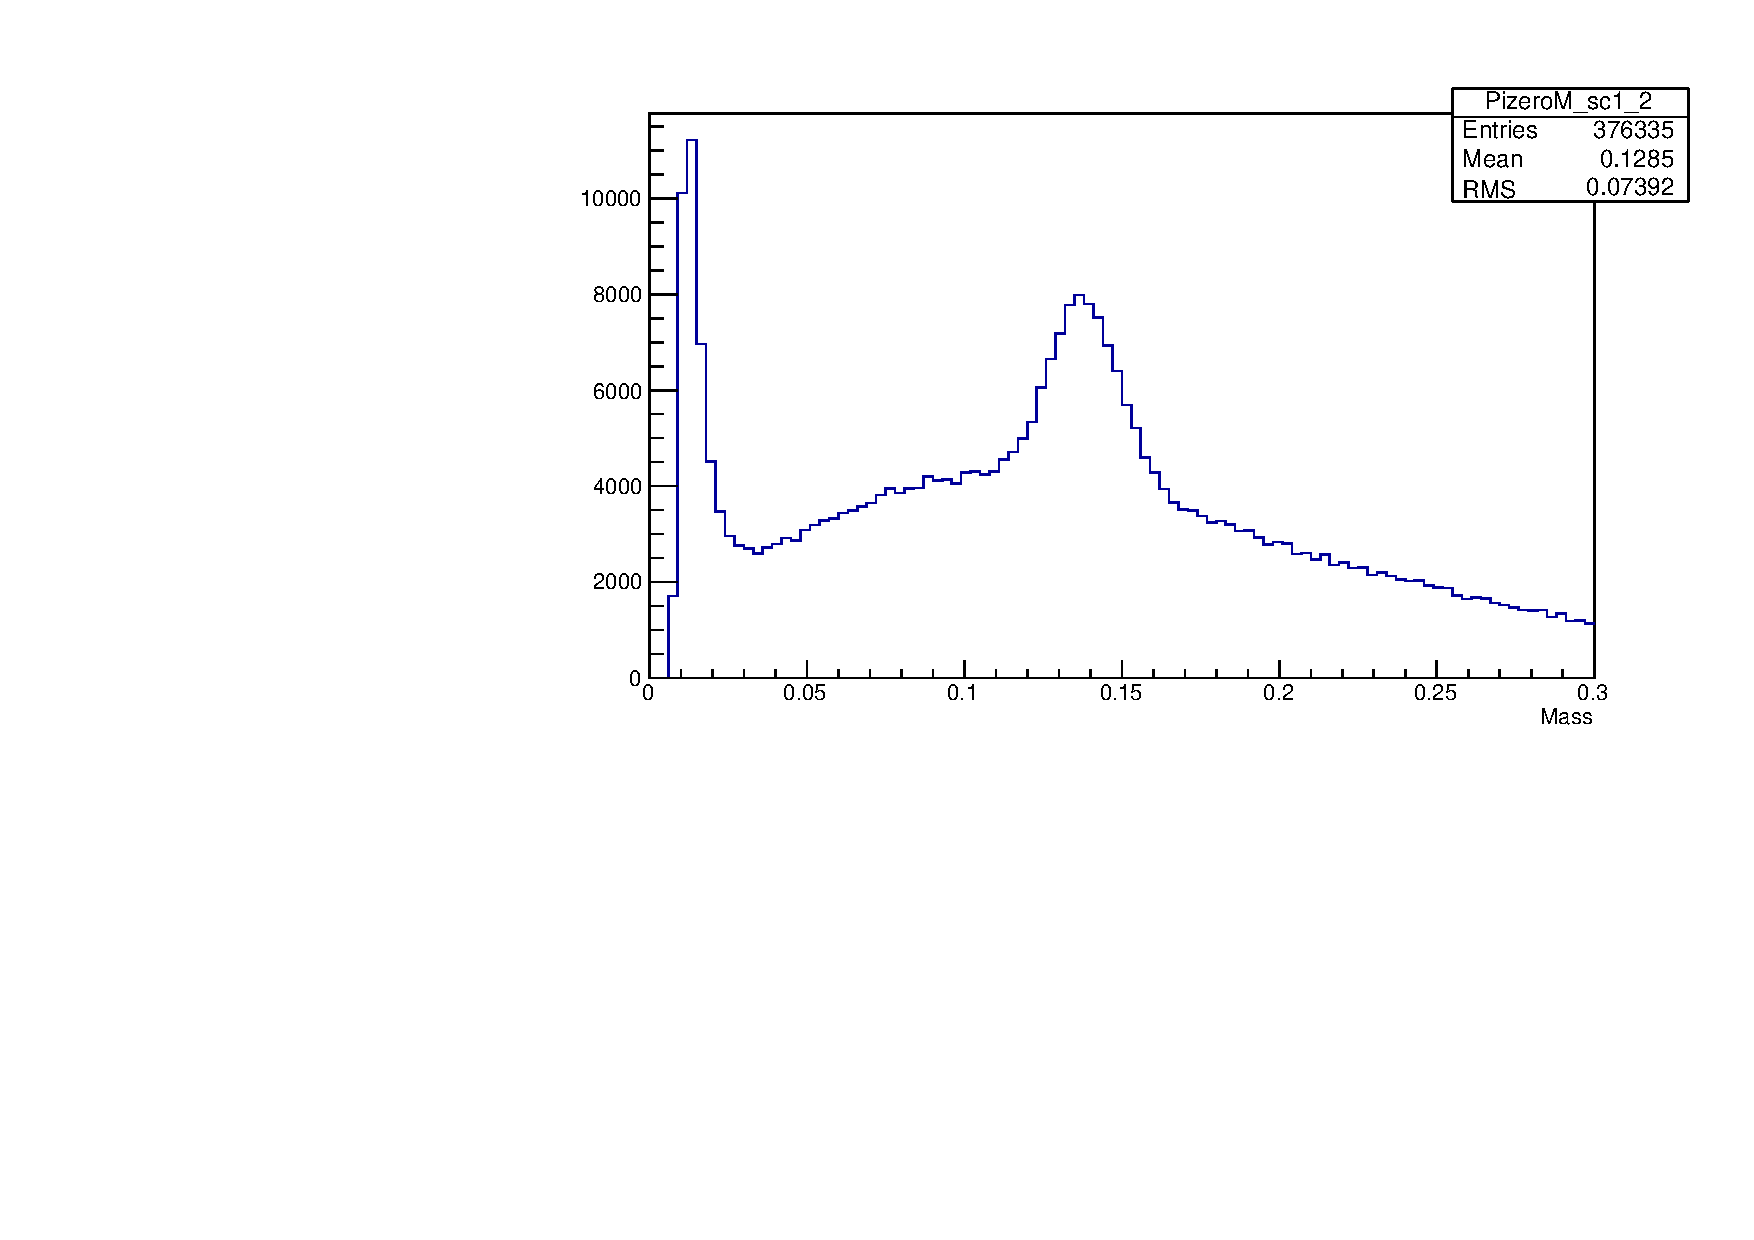
\includegraphics[width=0.47\textwidth]{fig_pi0vn/cut4_sect2allruns.pdf}
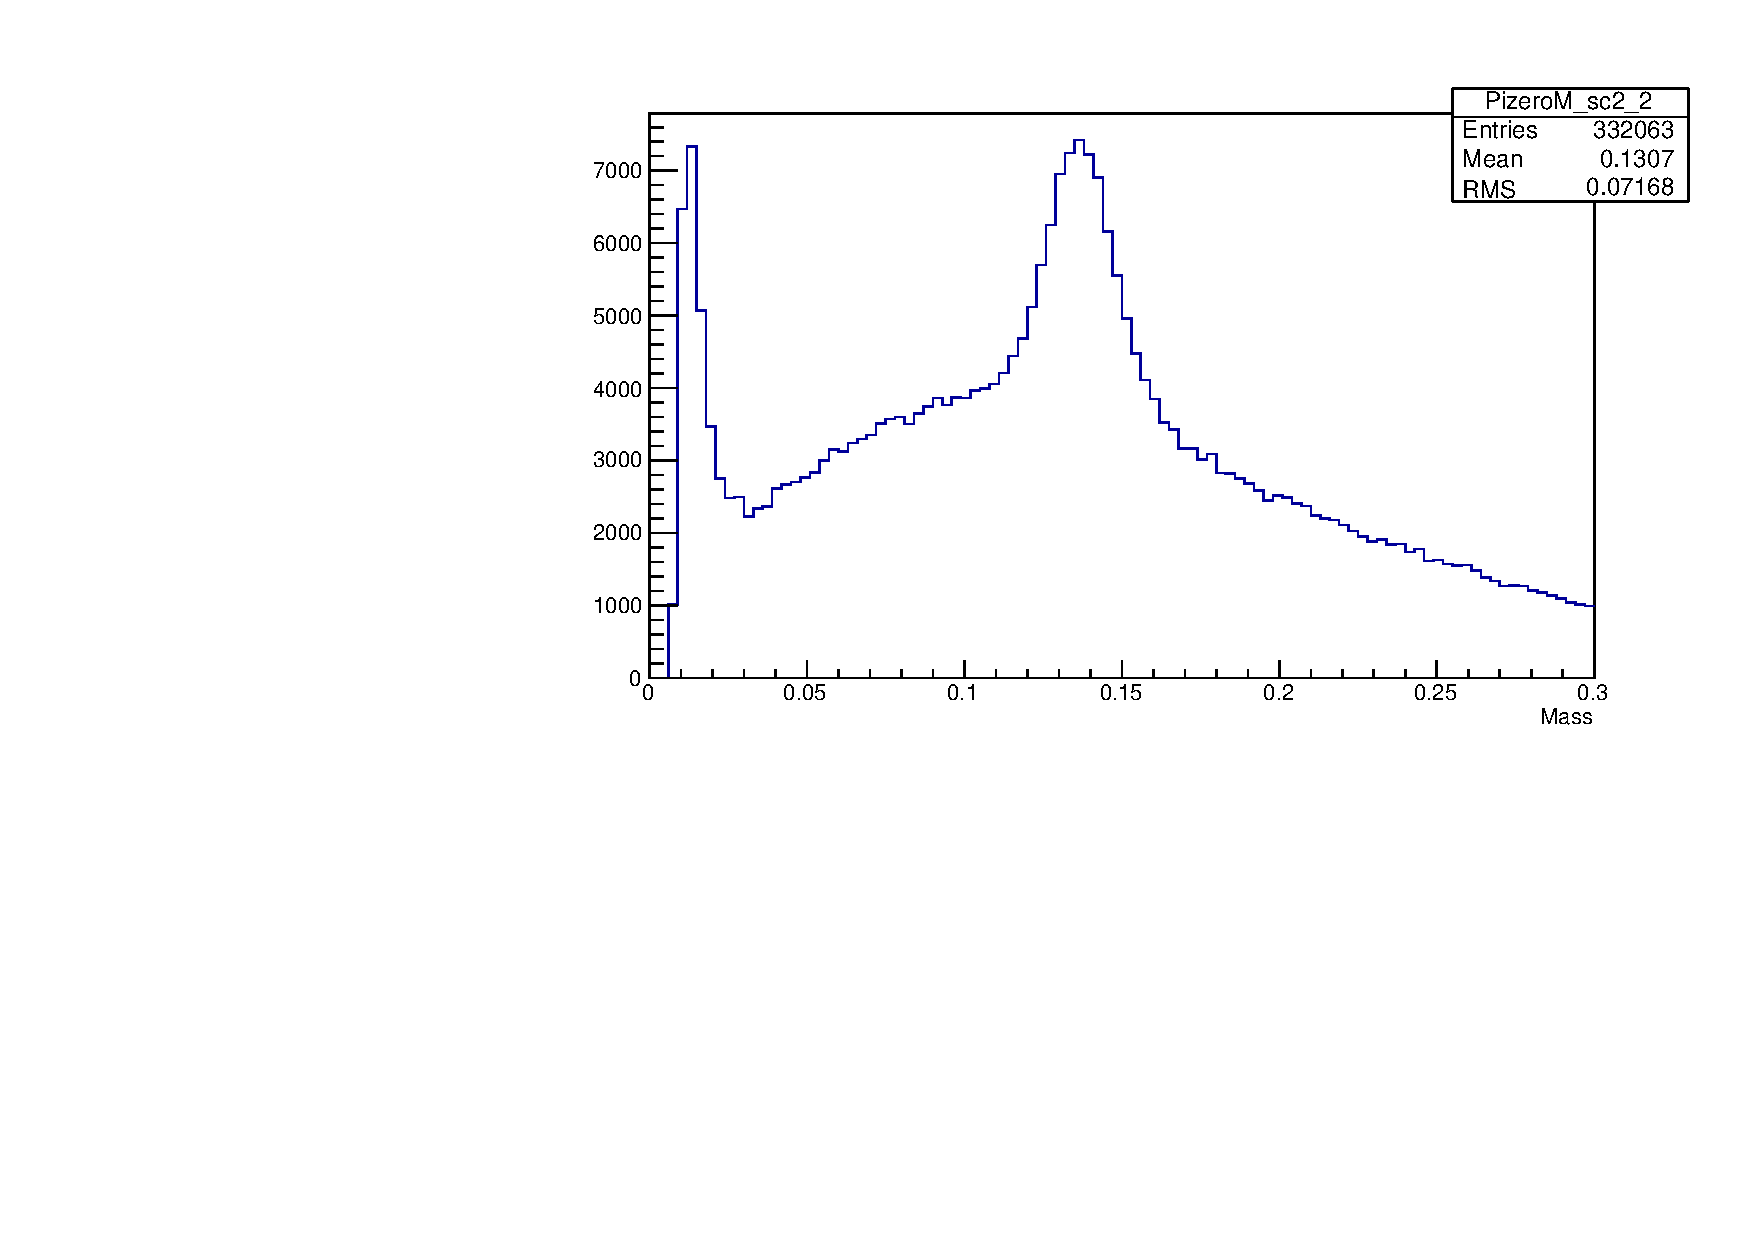
\includegraphics[width=0.47\textwidth]{fig_pi0vn/cut5_sect2allruns.pdf}
\label{invmasscuts}
\caption{}
\end{figure}

\section{EMCal QA Checks}
\subsection{MB trigger 200 GeV}
After to applied the dead/hot map and the energy calibration we look at some observables. Reminding we are doing basic cuts  $Ecore > 0.2 $ GeV, $\chi^2 < 3$ ,$zvtx<30$ cm.
 Figure \ref{clustervsrun200GeV_notiming} show the medium number of cluster per event and per sector versus the run number. Figure \ref{clusterpersector_withtiming} is the number of cluster per sector after do the timing cut $\vert T_{cluster} \vert <$ 5ns.
 \newline
 In figure \ref{meanpi0_notiming} shows the number of medium $\pi^{0}$ per event in invariant mass interval [0.135,0.141]GeV per sector, with $p_{t} > 1$ GeV, before timing cut, and figure \ref{meanpi0_withtiming} after timing cut.
 After the timing cut, there is still two runs that are out of the mean, so with do not use them for our analysis.
\begin{figure}
    \centering
    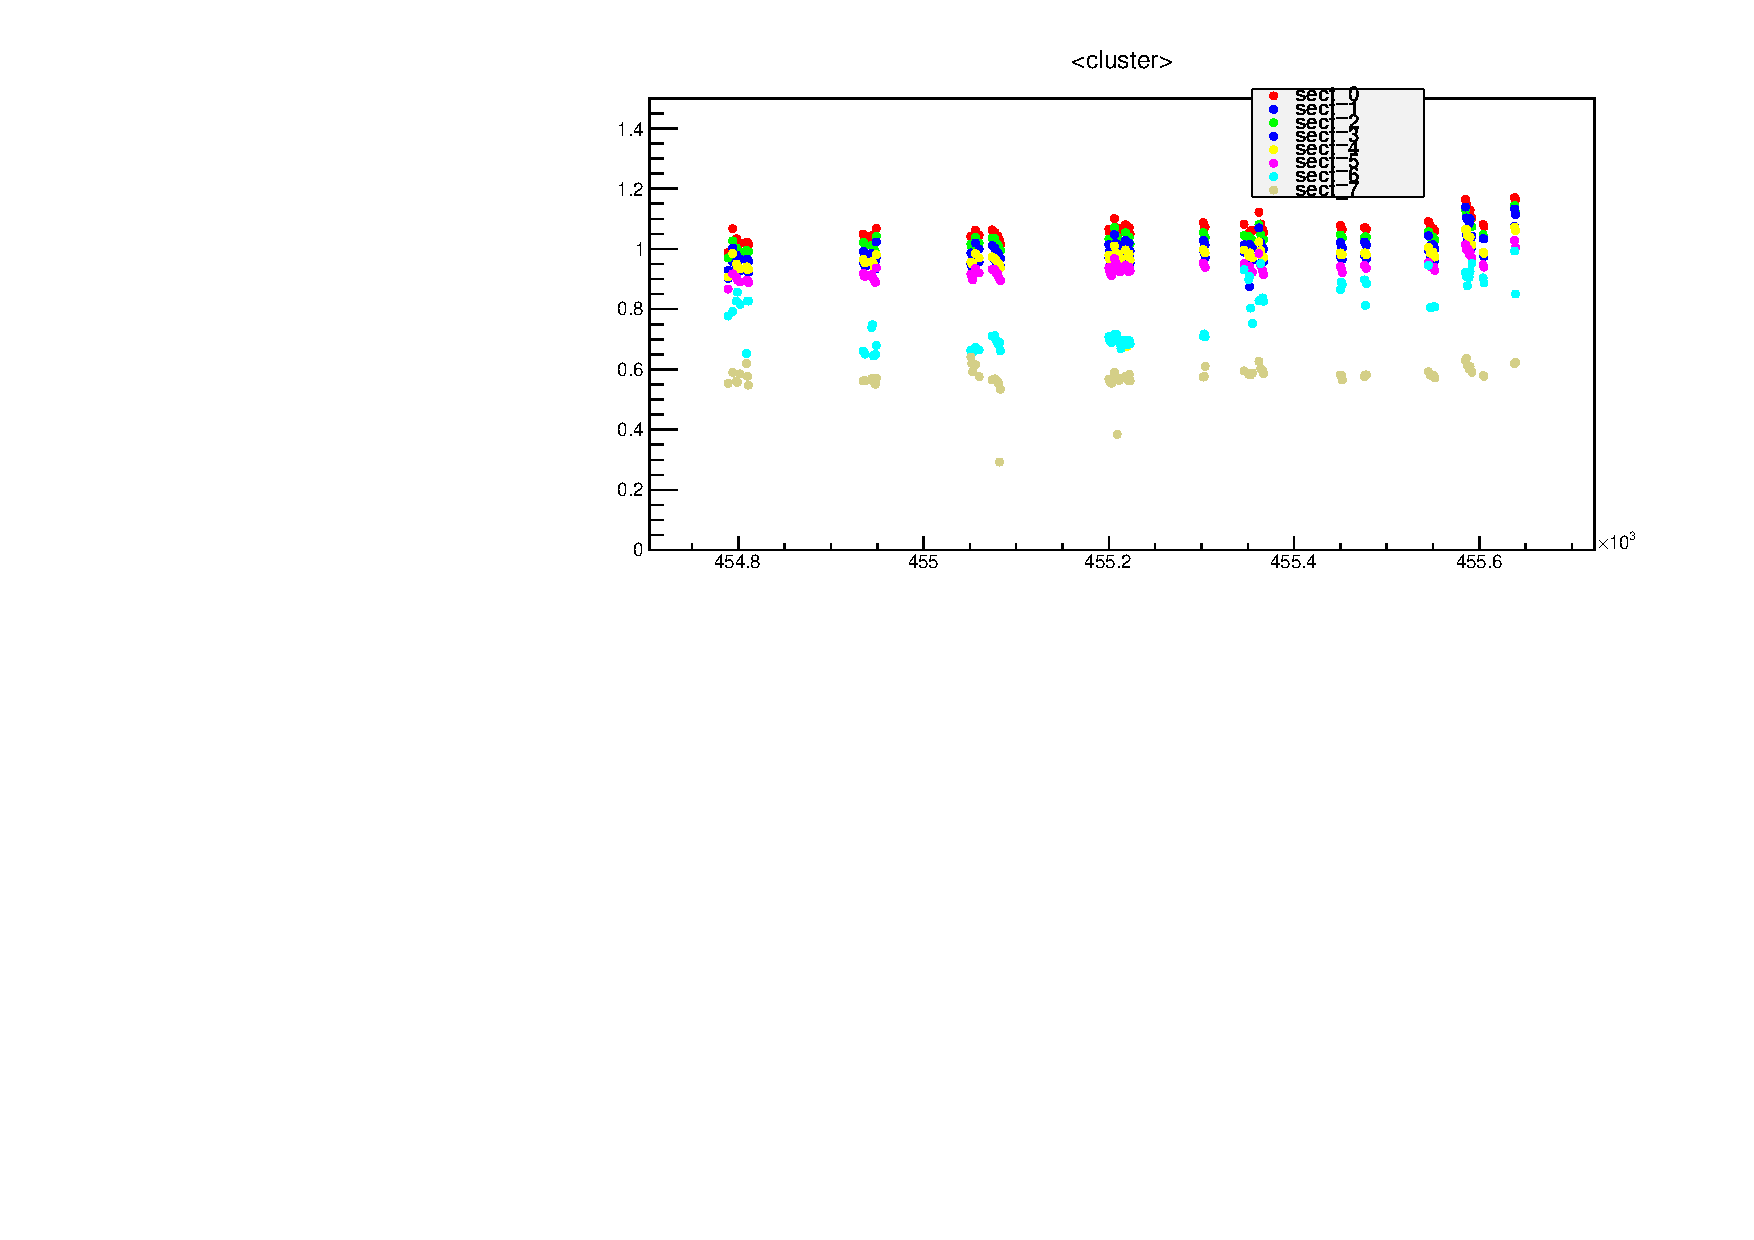
\includegraphics[width=1\textwidth]{fig_pi0vn/meancluster_notiming.pdf}
    \caption{dAu 200 GeV  medium number of cluster per event per sector versus run number}
    \label{clustervsrun200GeV_notiming}
\end{figure}
\begin{figure}
    \centering
    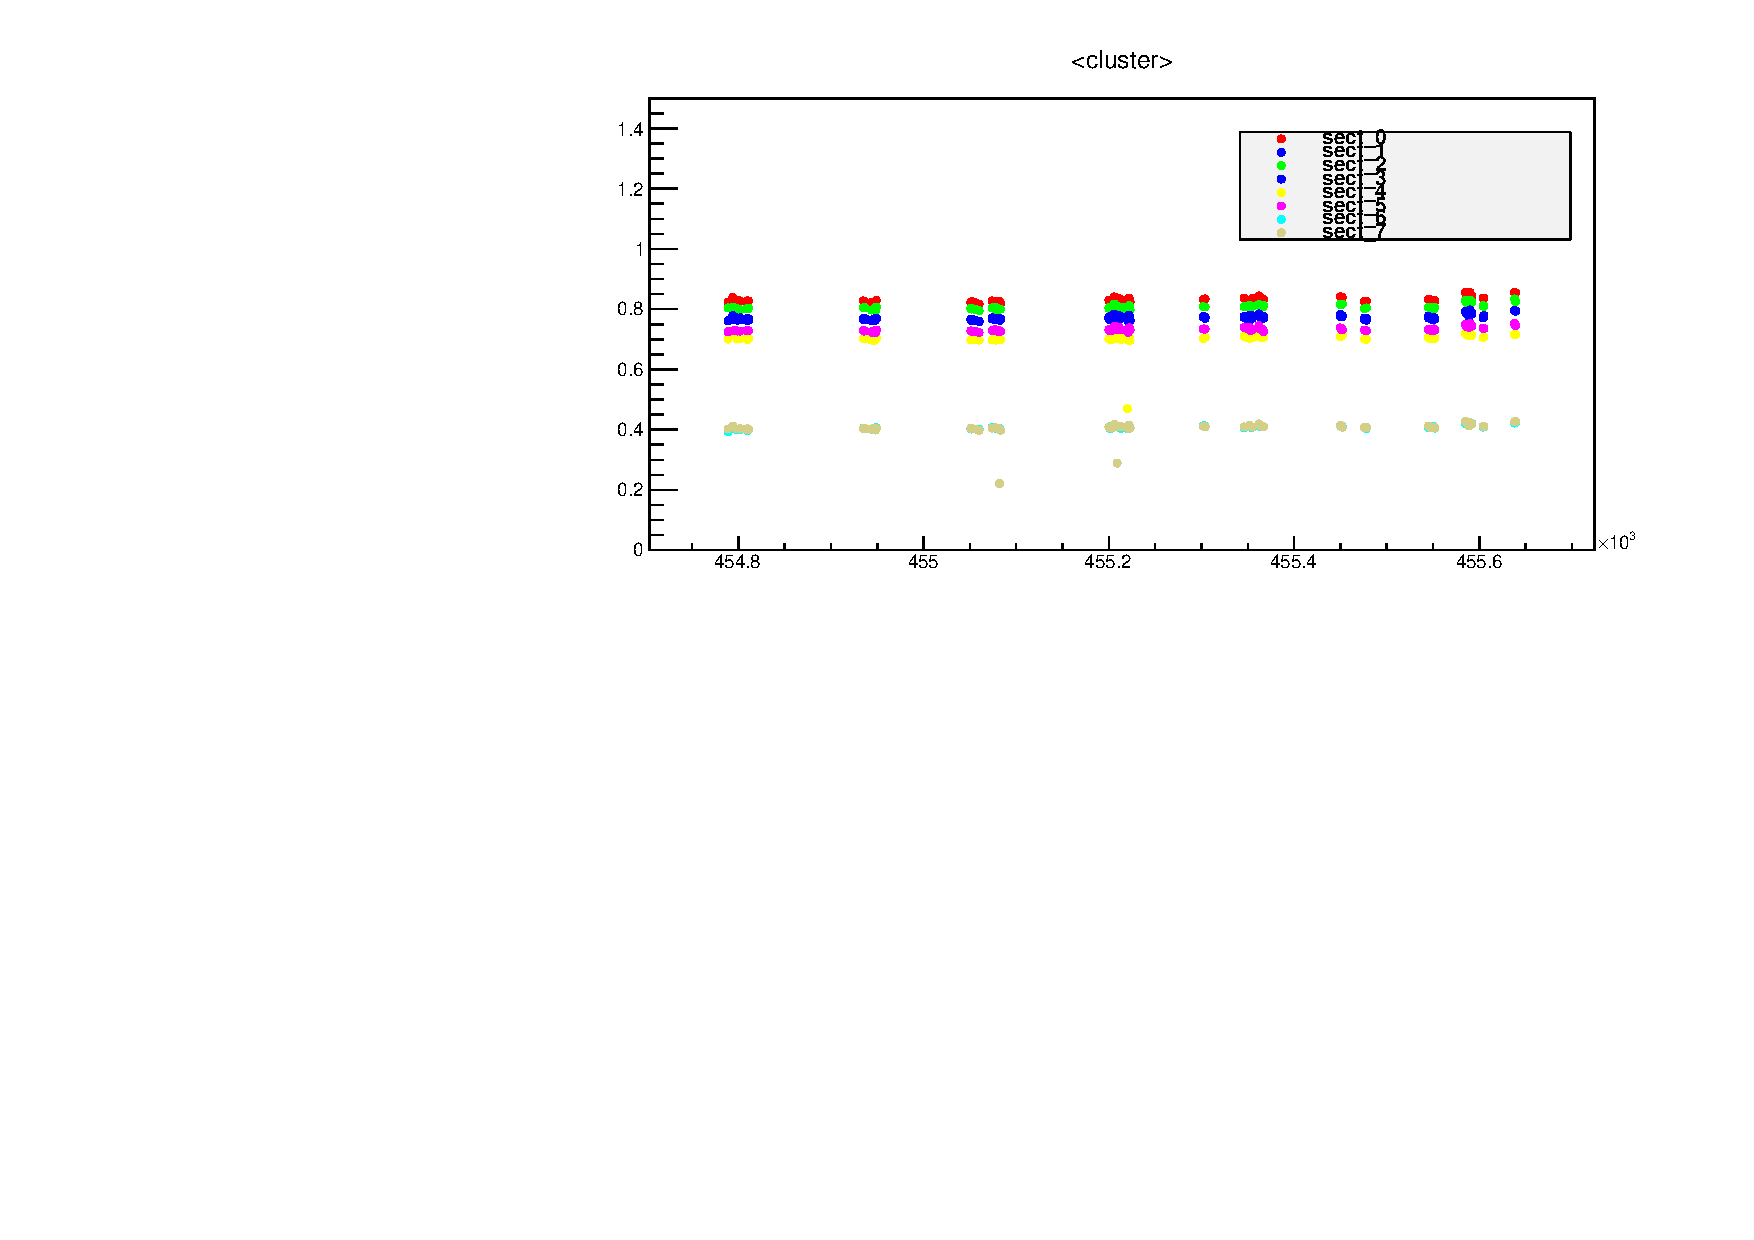
\includegraphics[width=1\textwidth]{fig_pi0vn/meancluster_withtiming.pdf}
    \caption{dAu 200 GeV  medium number of cluster per event for each sector versus run number}
    \label{clusterpersector_withtiming}
\end{figure}
\begin{figure}
    \centering
    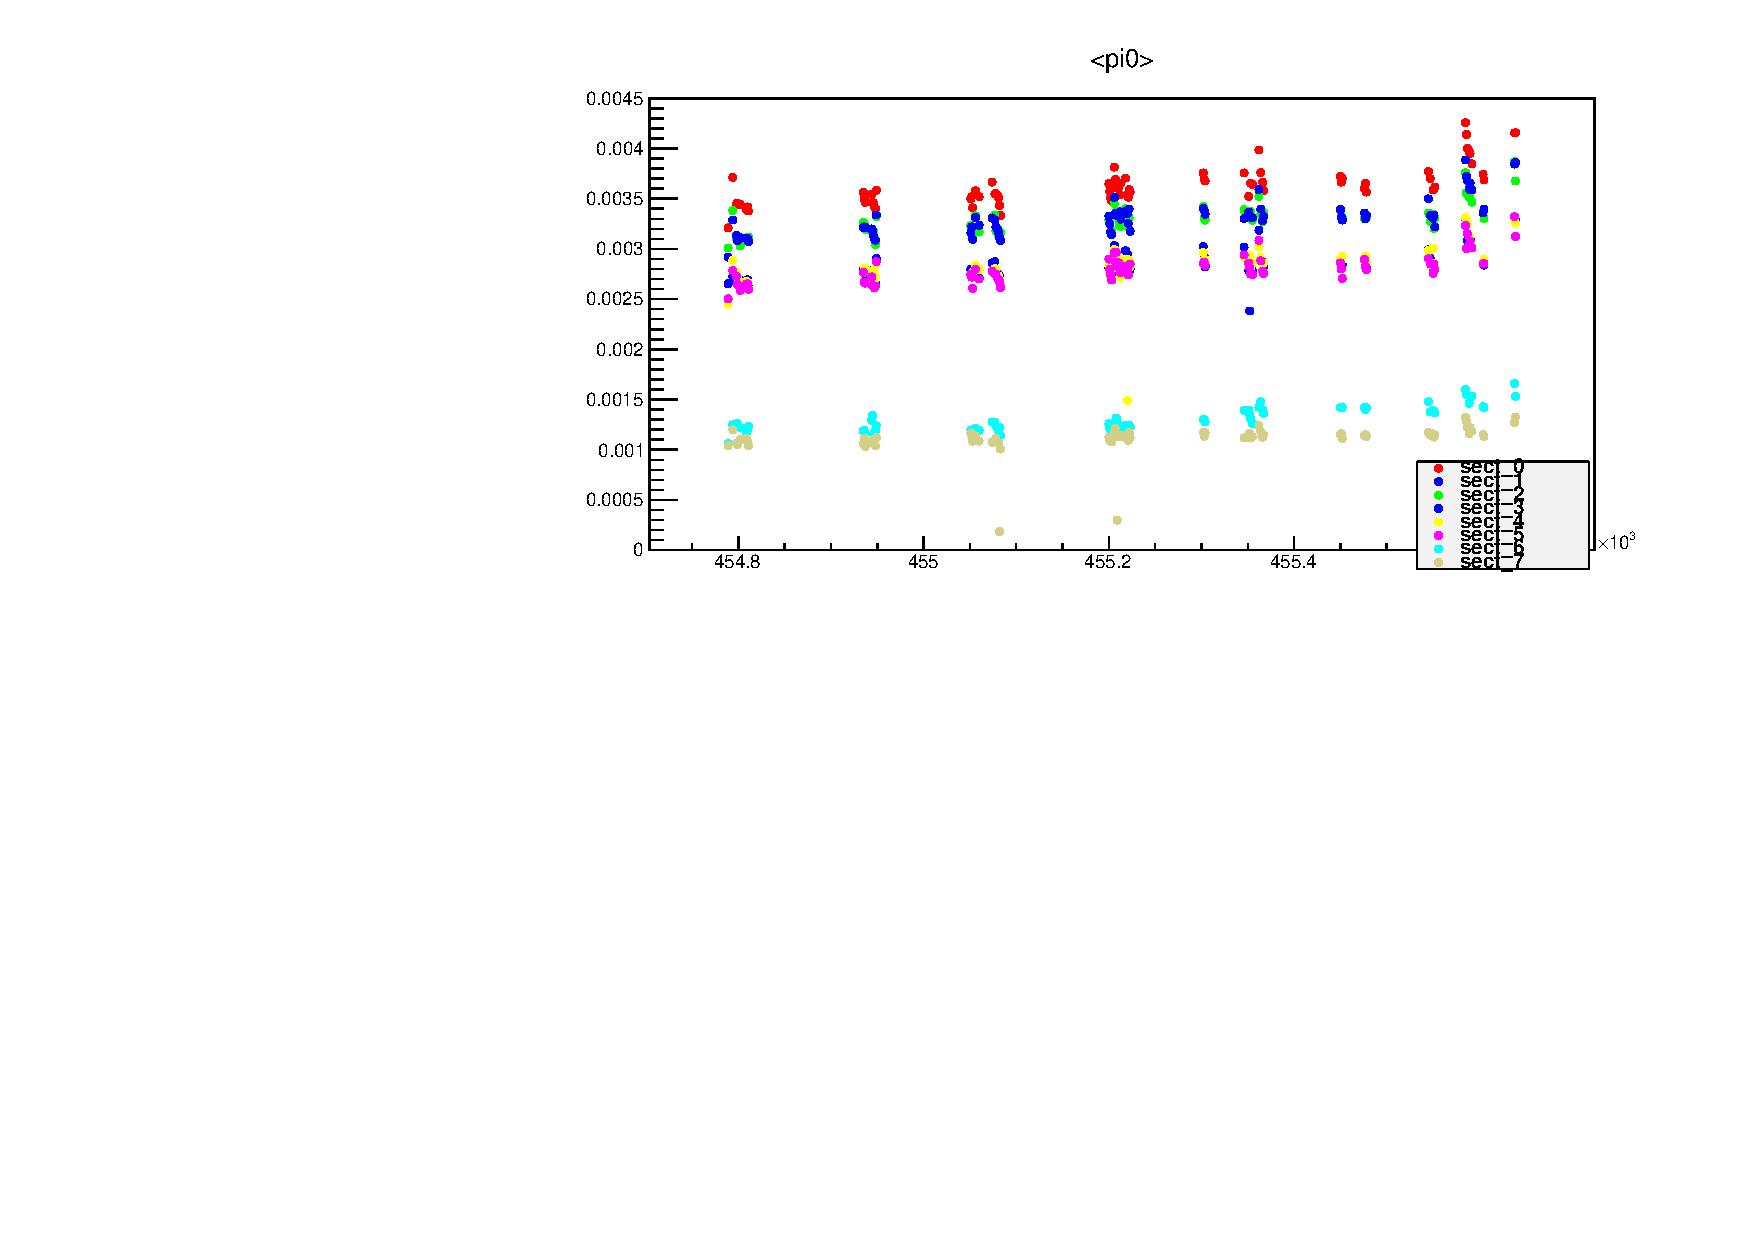
\includegraphics[width=1\textwidth]{fig_pi0vn/meanpi0_notiming.pdf}
    \caption{dAu 200 GeV  medium number of $\pi^{0}$ ($135 MeV <\pi^0 < 141 MeV$) per event for each sector versus run number for $p_{T}>1$ GeV}
    \label{meanpi0_notiming}
\end{figure}
\begin{figure}
    \centering
    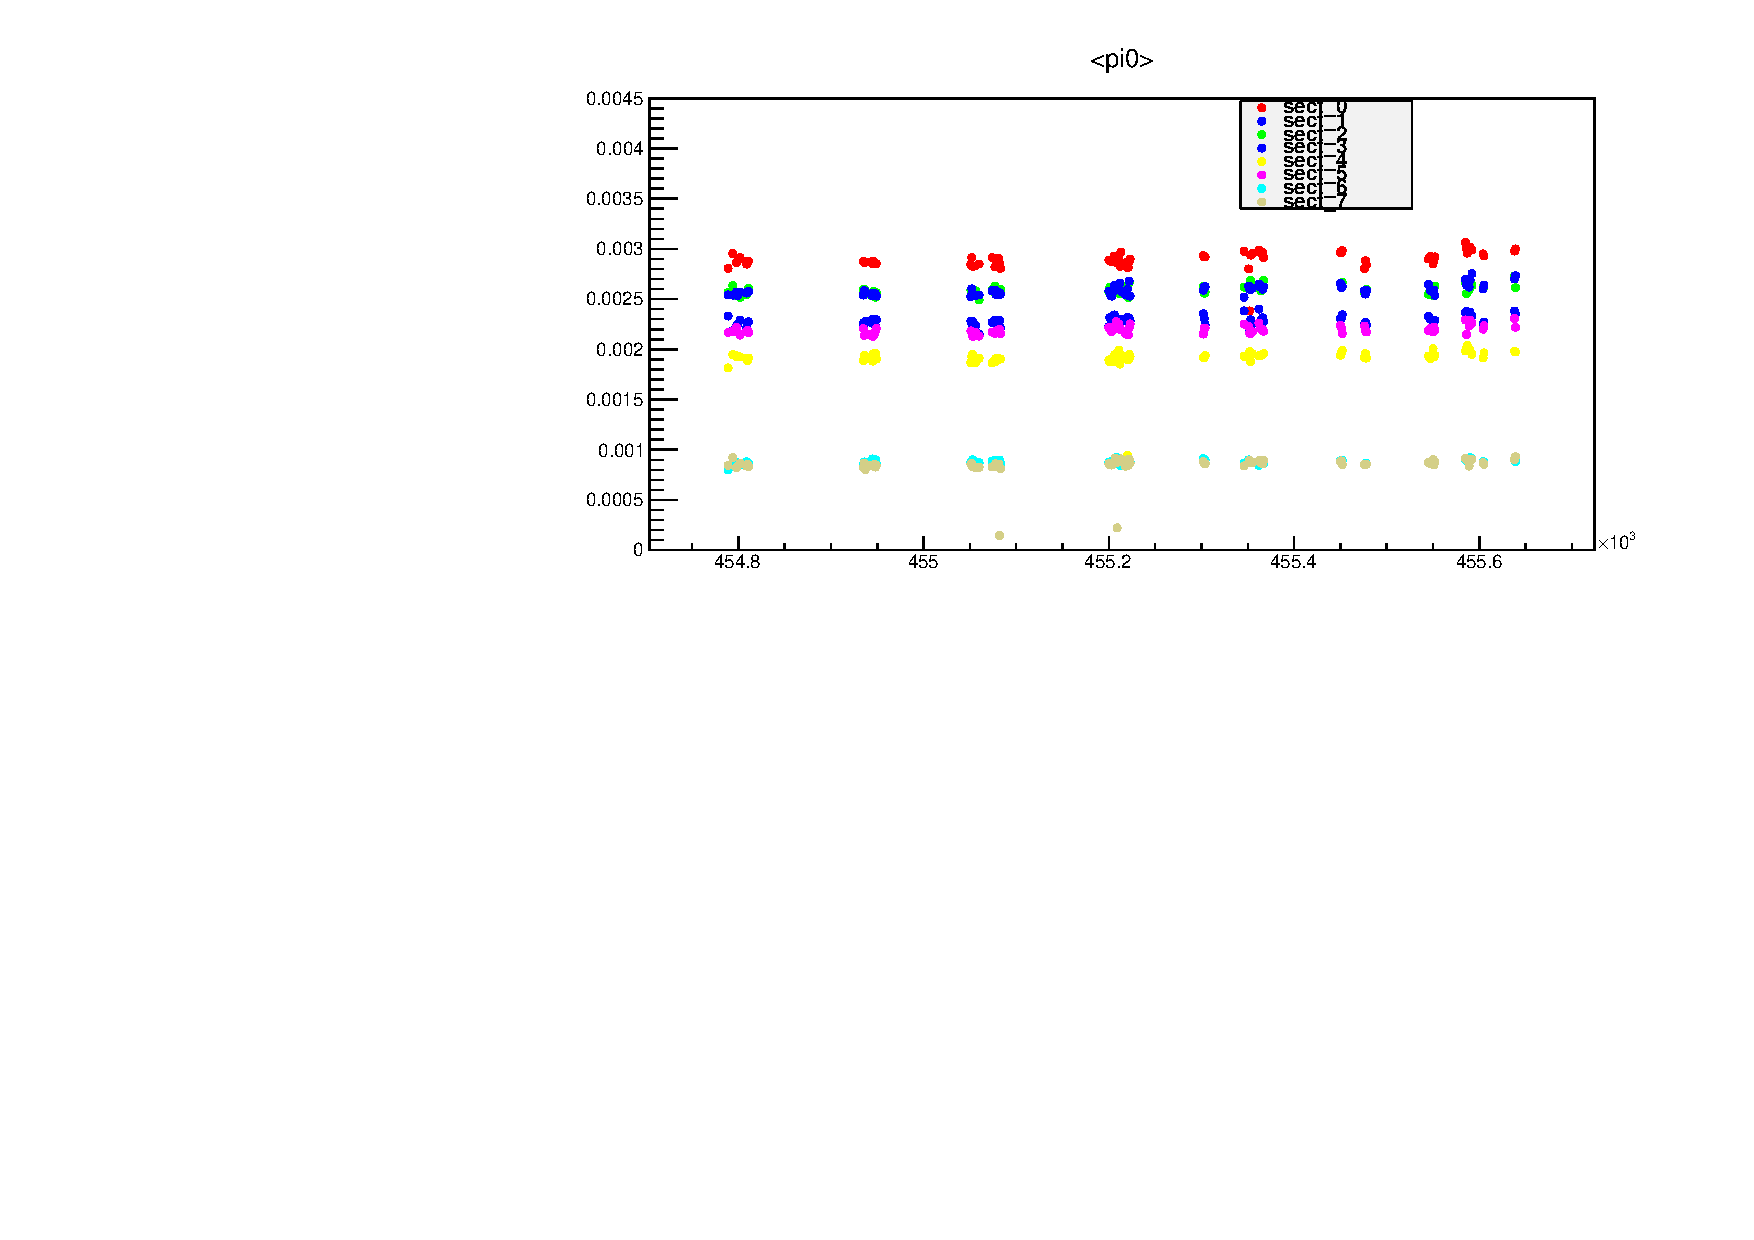
\includegraphics[width=1\textwidth]{fig_pi0vn/meanpi0_withtiming.pdf}
    \caption{dAu 200 GeV  medium number of pi0($135 MeV <\pi^0 < 141 MeV$) per event for each sector versus run number for $p_{T}>1$ GeV, with timing cut}
    \label{meanpi0_withtiming}
\end{figure}
\subsection{MB trigger 62 GeV}
\subsection{ERT trigger 200 GeV}

\section{Reference Flow}
For this analysis the reference flow detector is either BBC or MPCEX.
The calibration procedure consists of a gain equalization done over the whole detectors followed by four steps: Re-centering, Twist, Scale and Flattening.
This recipe is the same used in many RHIC and LHC publications and it is described in following sections.
\subsection{Q Vector Computation}
\label{subsection:Q Vector Computation}
The Q vector is an event-by-event observable defined as
\begin{center}
\large
$Q_{n}$ = $\sum_{i} \omega_{i} e^{in\phi_{i}}$ = $\vert Q_{n} \vert e^{in\Psi_{n}}$
\end{center}
where the sum goes over all particles in the sample and $\phi_{i}$ is the laboratory azimuthal angle of the particles emerging from the collision.
\newline
When the sample is composed of reconstructed particles, the weight $\omega_{i}$ is sometimes different than 1 in order to enhance 
the contribution of particles with the highest contribution to the flow, on the other hand, for some detector configurations 
(like BBC, FVTX and MPCEX) the weight $\omega_{i}$ is the relative energy.
\newline
The event plane $\Psi_{n}$ is the angle associated to the Q vector polar angle.
\begin{center}
\large
$\Psi_{n} = \frac{1}{n} tan^{-1}( \frac{Im(Q_{n})}{Re(Q_{n})} )$
\end{center}
\subsection{Q Vector Correction}
\begin{verbatim}
    https://www.phenix.bnl.gov/WWW/p/forms/info/show_note.php?editkey=an1406
\end{verbatim}
\label{subsection:Q Vector Correction}
The Q vector can be computed by any detector that has azimuthal granularity (trackers, hodoscopes, calorimeters, etc).
For a proper unbiased estimator, one needs to correct by detector non-uniform acceptance and efficiency.
The corrections used here are computed from the data itself and consist of several steps.
Further details can be found in analysis note AN1406.

\paragraph{Recentering the \textbf{Q} Centeroid}
\label{paragraph:Recentering the Q Centeroid}
\begin{center}
\large
$Q_{nx}^{I}$ = $Q_{nx}$(1 - $\langle$cos$n\phi$$\rangle$),   $Q_{ny}^{I}$ = $Q_{ny}$(1 -$\langle$sin$n\phi$$\rangle$)
\end{center}

\paragraph{Twist of the Q Vector}
\label{paragraph:Twist of the Q Vector}
\begin{center}
\large
$Q_{nx}^{II} = \frac{Q_{nx}^{I} - \lambda_{2n}^{s-}Q_{ny}^{I} }{1-\lambda_{2n}^{s-}\lambda_{2n}^{s+}}, Q_{ny}^{II} = \frac{Q_{ny}^{I} - \lambda_{2n}^{s+}Q_{nx}^{I} }{1-\lambda_{2n}^{s-}\lambda_{2n}^{s+}}, \lambda_{2n}^{s\pm} = \frac{\langle sin 2n\varphi \rangle}{1 \pm \langle cos 2n\varphi}$
\end{center}
\paragraph{Scaling the Q Vector}
\label{paragraph:Scaling the Q Vector}
\begin{center}
\large
$Q_{nx}^{III} = \frac{Q_{nx}^{II}}{1+\langle cos 2n\varphi \rangle}, Q_{ny}^{III} = \frac{Q_{nxy}^{II}}{1+\langle cos 2n\varphi \rangle}$
\end{center}

\paragraph{Flattening the event plane}
\label{paragraph:Flattening of the Q Vector}
\begin{center}
$\Psi_{n}^{IV} = \Psi_{n}^{III} + \sum_{m} \frac{2}{m}(-\langle sin m\Psi_{n}^{III} \rangle cos m\Psi_{n}^{III} + \langle cos m\Psi_{n}^{III} \rangle sin m \Psi_{n}^{III})$
\end{center}
\par
Each of these effects were corrected sequentially, which requires several passes over data.
Notice that if there were not any bias, each of the averages "$\langle$$\rangle$" would be zero and 
thus $Q^{IV}$ = $Q^{III}$ = $Q^{II}$ = $Q^{I}$ = Q we recover the original Q.
\subsection{MPCEX and FVTX Q Vectors}
\label{subsection:MPCEX and FVTX Q Vectors}
Each silicon pixel in MPCEX has size 2mm x 8mm, provide good $\phi$ granularity, thus has large advantage on measuring higher order 
Fourier moment. since MPCEX has hot/dead channels spread on each layer. we symmetrize by masking channels placed on the opposite side of 
bad channels, makes calibration easier. Figure \ref{fig:MPCEX Acceptance} describes how it's done. And MPCEX south covers similar $\eta$ range of BBC [-3.8, -3.1].
FVTX is disk-shaped detector assembling the silicon 'wedges' that covers $7.5^{\circ}$ $\phi$ angle per each, almost symmetric 
with respect to $\phi$.
FVTX covers \textless  $\vert \eta \vert$ \textless 2.2 region.
We calibrated MPCEX, FVTX by recentering and flattening technique (Fig \ref{fig:EP Calibration for Detectors}) and checked correlation between MPCEX, $BBC_{A}$, $BBC_{B}$, 
FVTX (Fig \ref{fig:EP Correlation}). We found BBC has the largest statistics and fair size of EP resolution, used as the primary event plane detector.
\newline

\begin{figure}[!htb]
  \centering  
    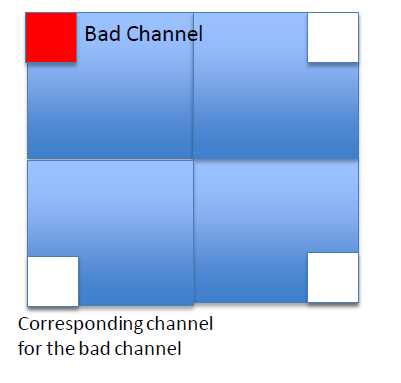
\includegraphics[width=0.44\textwidth]{fig_pi0vn/mpcex_symmetrize.PNG}
    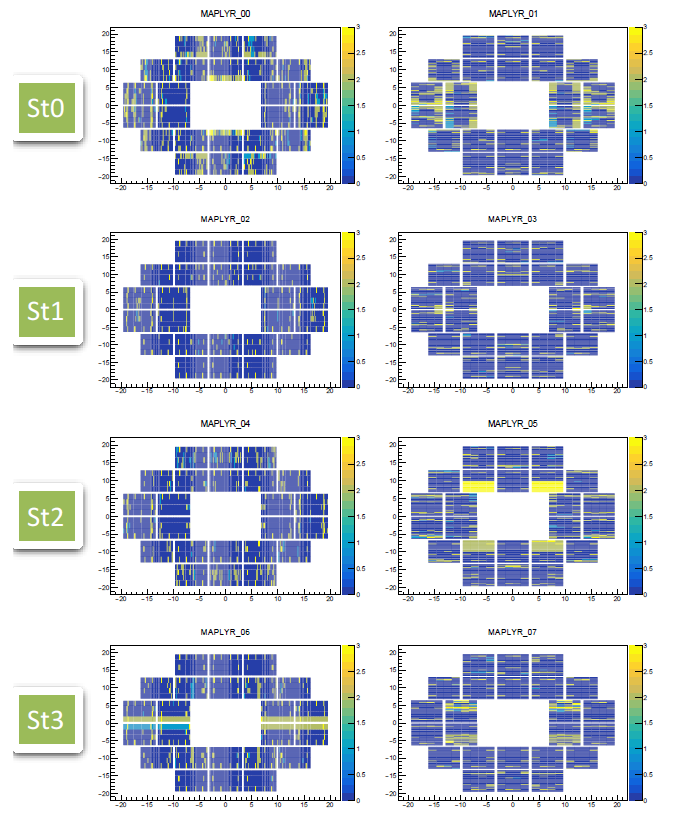
\includegraphics[width=0.5\textwidth]{fig_pi0vn/mpcex_acceptance.PNG}
  \caption[MPCEX appetance]{MPCEX symmetrization (left) red spot is bad channels and white is masked area, MPCEX acceptance after masking (right), yellow 
  areas are masked area}
  \label{fig:MPCEX Acceptance}
\end{figure}

\begin{figure}[!htb]
  \centering  
    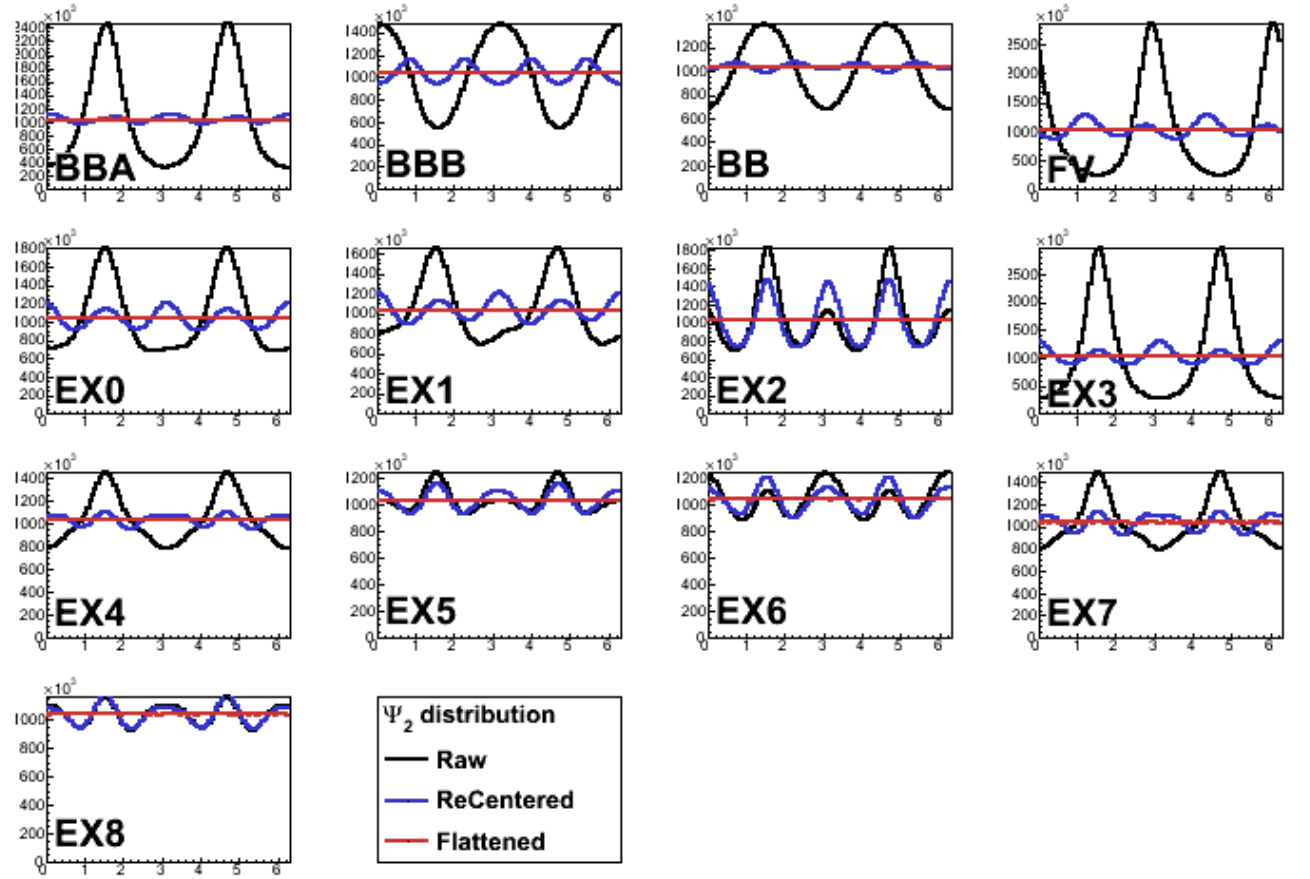
\includegraphics[width=\textwidth]{fig_pi0vn/epcalib_mpcex_fvtx.PNG}
  \caption[d+Au200GeVMB centrality $0-5\%$, 2nd order EP Calibration]{Run16dAu200GeVMB centrality $0-5\%$, 2nd order EP Calibration, recentering and flattening has applied on FVTX, MPCEX(Layer), 
  $BBC_{A}$, $BBC_{B}$}
  \label{fig:EP Calibration for Detectors}
\end{figure}

\begin{figure}[!htb]
  \centering  
    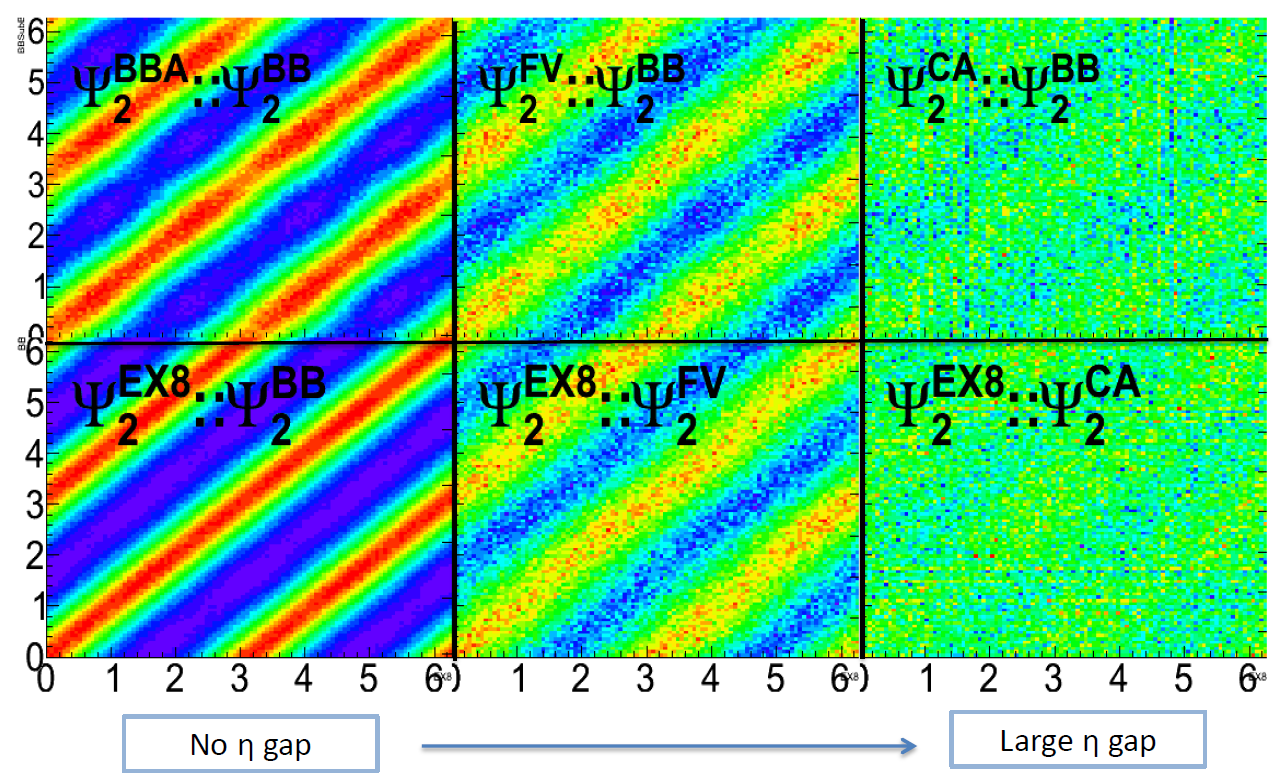
\includegraphics[width=\textwidth]{fig_pi0vn/ep_correlation.PNG}
  \caption[d+Au200GeVMB centrality $0-5\%$, EP Correlation]{Run16dAu200GeVMB centrality $0-5\%$, EP Correlation, 2nd order EP Correlation between BBC, FVTX, MPCEX(Layer).}
  \label{fig:EP Correlation}
\end{figure}

\section{Data analysis}
\subsection{Analysis Chain}
\subsection{Systematic Errors}
\section{Results}
\section{Appendix}
\subsection{Data tables}
\subsection{Run List}
The list of runs used for BBC based results are:

Run16dAu200GeV Minimum bias data
\newline
454777, 454778, 454782, 454783, 454784, 454785, 454786, 454789,
454794, 454797, 454798, 454799, 454800, 454802, 454808, 454809,
454810, 454811, 454933, 454934, 454935, 454936, 454937, 454943, 
454944, 454945, 454946, 454947, 454948, 455049, 455050, 455051, 
455052, 455053, 455056, 455060, 455062, 455063, 455064, 455065, 
455066, 455071, 455073, 455074, 455077, 455078, 455080, 455081, 
455082, 455083, 455200, 455201, 455202, 455203, 455206, 455207, 
455208, 455209, 455211, 455212, 455213, 455218, 455220, 455221, 
455222, 455223, 455224, 455302, 455303, 455304, 455306, 455344, 
455346, 455351, 455352, 455353, 455355, 455362, 455363, 455364, 
455366, 455367, 455446, 455449, 455450, 455451, 455452, 455476, 
455477, 455478, 455545, 455547, 455550, 455551, 455552, 455585, 
455586, 455587, 455589, 455590, 455592, 455604, 455605, 455637, 
455638, 455639 

Run16dAu200GeV ERT Data
\newline
454774, 454777, 454778, 454782, 454783, 454784, 454785, 454786,
454789, 454794, 454797, 454798, 454799, 454800, 454802, 454808,
454809, 454810, 454811, 454933, 454934, 454935, 454936, 454937,
454943, 454944, 454945, 454946, 454947, 454948, 455049, 455050,
455051, 455052, 455053, 455056, 455060, 455071, 455073, 455074,
455077, 455078, 455080, 455081, 455082, 455083, 455200, 455201,
455202, 455203, 455206, 455207, 455208, 455209, 455211, 455212,
455213, 455218, 455220, 455221, 455222, 455223, 455224, 455302,
455303, 455304, 455306, 455344, 455346, 455351, 455352, 455353, 
455355, 455362, 455363, 455364, 455366, 455367, 455446, 455449,
455450, 455451, 455452, 455476, 455477, 455478, 455545, 455547,
455550, 455551, 455552, 455585, 455586, 455587, 455589, 455590,
455592, 455604, 455605, 455637, 455638, 455639
\end{document}

